%; whizzy paragraph
%; whizzy-paragraph "^\\\\dancersection"
% -initex iniptex -latex platex -format platex -bibtex jbibtex -fmt fmt
% 以上 whizzytex を使用する場合の設定。

%     Tokyo Debian Meeting resources
%     Kansai Debian Meeting resources
%     Copyright (C) 2008 Junichi Uekawa
%     Copyright (C) 2008 Nobuhiro Iwamatsu

%     This program is free software; you can redistribute it and/or modify
%     it under the terms of the GNU General Public License as published by
%     the Free Software Foundation; either version 2 of the License, or
%     (at your option) any later version.

%     This program is distributed in the hope that it will be useful,
%     but WITHOUT ANY WARRANTY; without even the implied warranty of
%     MERCHANTABILITY or FITNESS FOR A PARTICULAR PURPOSE.  See the
%     GNU General Public License for more details.

%     You should have received a copy of the GNU General Public License
%     along with this program; if not, write to the Free Software
%     Foundation, Inc., 51 Franklin St, Fifth Floor, Boston, MA  02110-1301 USA

%   Pdf作成手順
% dvipdfmx debianmeetingresume2011-fuyu.dvi
%  preview (shell-command (concat "evince " (replace-regexp-in-string "tex$" "pdf"(buffer-file-name)) "&"))
% 画像ファイルを処理するためにはebbを利用してboundingboxを作成。
%(shell-command "cd image2012-fuyu; ebb *.png")


% progress memo:
% 2011/6-2011/11がマージ対象、関西は2011/6-2011/11(仮)
% イベント等でない場合は理由を書くこと。
% 必要な変更点は FIXME で記録しています。

%%ここからヘッダ開始。

\documentclass[mingoth,a4paper]{jsarticle}
\usepackage{monthlyreport}
\usepackage[dvips]{xy} % for advi workaround. Bug #452044
\usepackage{iwamatsu}

\begin{document}

\begin{titlepage}
\thispagestyle{empty}

\hspace*{-2.5cm}
\includegraphics{image2012-natsu/gudeb.eps}\\
\\
\\
\rotatebox{10}{\fontsize{32}{32} {\gt 東京エリア/関西Debian勉強会}}

%\vspace*{-1.5cm}
\hspace*{11cm}
\includegraphics[height=6cm]{image200502/openlogo-nd.eps}\\
\vspace*{0.1cm}
\hfill あんどきゅめんてっど でびあん 2012年冬号 2012年12月31日 初版発行
\end{titlepage}

\newpage
\thispagestyle{empty}\mbox{}
\newpage

% section の代わりの環境 -- 改訂する。
\renewcommand{\dancersection}[2]{%
\newpage
あんどきゅめんてっど でびあん 2012年冬号
%
% top line
\vspace{0.1mm}\\
{\color{dancerlightblue}\rule{\hsize}{2mm}}

%
% middle text
%
\begin{minipage}[t]{0.6\hsize}
\color{dancerdarkblue}
\vspace{1cm}
\section{#1}
\hfill{}#2\\
\end{minipage}
\begin{minipage}[t]{0.4\hsize}
\vspace{-2cm}
\hfill{}
\includegraphics[height=8cm]{image200502/openlogo-nd.eps}\\
\vspace{-5cm}
\end{minipage}
%
%
{\color{dancerdarkblue}\rule{0.74\hsize}{2mm}}
%
\vspace{2cm}
}

\setcounter{page}{1}
\begin{minipage}[]{0.2\hsize}
 \definecolor{titleback}{gray}{0.9}
 \colorbox{dancerlightblue}{\rotatebox{90}{\fontsize{80}{80}
{\gt \color{dancerdarkblue}デビアン勉強会} }}
\end{minipage}
\begin{minipage}[]{0.8\hsize}
\hrule
\vspace{1mm}
\hrule
\setcounter{tocdepth}{1}
{\small
 \tableofcontents}
\vspace{1mm}
\hrule
\vspace{3cm}

\end{minipage}

% FIXME: 本文を追加すること。
%-------------------------------------------------------------------------------
\dancersection{Introduction}{DebianJP}
%-------------------------------------------------------------------------------

\subsection{東京エリアDebian勉強会}

 Debian勉強会へようこそ。これからDebianの世界にあしを踏み入れると
 いう方も、すでにどっぷりとつかっているという方も、月に一回Debianについ
 て語りませんか?

 Debian勉強会の目的は下記です。

\begin{itemize}
 \item \underline{Debian Developer} (開発者)の育成。
 \item 日本語での ``\underline{開発に関する情報}'' を整理してまとめ、アップデートする。
 \item \underline{場}の提供。
 \begin{itemize}
  \item 普段ばらばらな場所にいる人々が face-to-face で出会える場を提供
	する。
  \item Debian のためになることを語る場を提供する。
  \item Debianについて語る場を提供する。
 \end{itemize}
\end{itemize}

 Debianの勉強会ということで究極的には参加者全員がDebian Packageをがりがり
 と作るスーパーハッカーになった姿を妄想しています。情報の共有・活用を通し
 て Debianの今後の能動的な展開への土台として、 ``場'' としての空間を提供す
 るのが目的です。

\subsection{関西 Debian 勉強会}

 関西 Debian 勉強会はDebian GNU/Linux のさまざ
 まなトピック(新しいパッケージ、Debian 特有の機能の仕組、Debian 界隈で起
 こった出来事、などなど)について話し合う会です。

 目的として次の三つを考えています。
 \begin{itemize}
  \item MLや掲示板ではなく、直接顔を合わせる事での情報交換の促進
  \item 定期的に集まれる場所
  \item 資料の作成
 \end{itemize}

 それでは、楽しい一時をお楽しみ下さい。

%-------------------------------------------------------------------------------
\dancersection{MacBook Air 4,1 (Mid 2011)にDebianインストールしてみた}{上川 純一}
%-------------------------------------------------------------------------------
\index{macbook air}

\subsection{はじめに}

AppleのMacBook Airなどの製品は通常のPCとは違い起動がEFI経由でなされるな
どの癖があります。
久しぶりにどうやってインストールして動かすのかについてまとめてみました紹
介します。
今回はrEFIt\cite{refit}経由でgrub-pcを利用する Mac OS X との dual boot 構成にしています。

\subsection{インストール開始からDual Bootで起動するまで}
\index{refit}
\index{efi}

まず、Mac OS Xがディスク全体を利用しているため、インストールできるスペースがありません。
Mac OS Xのコマンドラインからdiskutil resizevolumeを使ってディスクを小さ
くします。

\begin{commandline}
 # sudo diskutil resizevolume disk0s2 30G 
\end{commandline}

Mac の起動はBIOSではなくEFI経由なのですが、rEFItはEFIで起動するブートローダーです。メニュー形式やコマンドラインでGrubをチェーンロードしたりできます。
Mac OSでrEFItをインストールします。最近のrEFIt はインストーラーに従うと
自動でインストールしてくれるようになっているようで自分でBlessコマンドを
うったりする必要はありません。

何度か再起動すると起動時にrEFItの画面に切り替わるようになるようです。

Debian Installerの名刺サイズのISOイメージをUSBメモリ\footnote{僕は今回は
USB SD リーダーに余ったmicro SDをさして使いました。}にddで書き込んでおくと、
再起動したときにrEFItからdebian installerを起動する選択肢が出てきます。

インストールは通常のように行います。
引っかかる場所は二箇所。Grubのインストールの部分とネットワークの設定でしょ
う。

無線ネットワークの brcmsmac ドライバが対応しているのですが、ファームウェ
アが必要でNon-freeのためインストーラに標準で入っていません。インストーラ用にファームウェ
アを事前に用意する必要がありますが、僕は面倒だったのでUSB Ethernetをつな
げてインストールしてしまいました。

Grubのインストールの部分はうまく行かず試行錯誤してしまったのですが、
refit パッケージにあるgptsyncコマンドを実行してGPTとFATのパーティションテー
ブルを同期させ、grub-pcをDebian installerがつくった小さなパーティションに
インストールすることで解決しました。多分コマンドラインはこんな感じだった
と思います。\footnote{grub-efi で BIOSエミュレーションではなくEFIモードを
使い起動し、GPTから直接ブートできるはずだと思われるのですが未確認。一部
のより新しいハードウェアではEFIモードで直接起動するほうがうまくうごくデバイスなど
があるらしい。}
Debian installerのシェルの中でtargetにchrootして作業しました。

 \begin{commandline}
# gptsync
# grub-install (hd0,4)
 \end{commandline}

\subsubsection{ディスクパーティション構成}
\index{gptsync}

GPT / FAT のパーティション構成は結果として次のようになりました。

 \begin{commandline}
$ cat /proc/partitions 
major minor  #blocks  name

   8        0  245117376 sda
   8        1     204800 sda1  # EFI
   8        2   39062500 sda2  # Mac OS X
   8        3     634768 sda3  # Mac OS X recovery?
   8        4        977 sda4  # grub
   8        5  197461914 sda5  # /
   8        6    7752380 sda6  # swap

$ sudo fdisk -l /dev/sda

WARNING: GPT (GUID Partition Table) detected on '/dev/sda'! The util fdisk doesn't support GPT. Use GNU Parted.


Disk /dev/sda: 251.0 GB, 251000193024 bytes
255 heads, 63 sectors/track, 30515 cylinders, total 490234752 sectors
Units = sectors of 1 * 512 = 512 bytes
Sector size (logical/physical): 512 bytes / 512 bytes
I/O size (minimum/optimal): 512 bytes / 512 bytes
Disk identifier: 0x0000221d

   Device Boot      Start         End      Blocks   Id  System
/dev/sda1               1      409639      204819+  ee  GPT
/dev/sda2          409640    78534639    39062500   af  HFS / HFS+
/dev/sda3        78534640    79804175      634768   ab  Darwin boot
/dev/sda4   *    79804176    79806129         977   c0  Unknown
 \end{commandline}

Mac OS XのパーティションはLinuxからはhfsplusファイルシステムとしてマウントすることができます。

 \begin{commandline}
sudo mount /dev/sda2 /mnt/ -o ro
$ mount -v 
/dev/sda2 on /mnt type hfsplus (ro,relatime,umask=22,uid=0,gid=0,nls=utf8)
 \end{commandline}

\subsection{無線LAN}
\index{brcmsmac}
\index{non-free firmware}

brcmsmac ドライバで無線LANは動きます。
non-free firmware が動作に必要になります。自由じゃないBinary Blobなどけ
しからんですが、non-free にパッケージがあるのでインストールしておけばうごきます。

 \begin{commandline}
ii  firmware-brcm80211          0.35                        Binary firmware for Broadcom 802.11 wireless cards
 \end{commandline}

\subsection{X}

\subsubsection{画面}

Wheezyに入っているLinuxカーネル3.2だとそのままいい解像度で動いてくれます。
xorgとしては\texttt{Integrated Graphics Chipset: Intel(R) Sandybridge
Mobile (GT2)}を認識してくれているようです。

 \begin{commandline}
$ xrandr
Screen 0: minimum 320 x 200, current 1366 x 768, maximum 8192 x 8192
eDP1 connected 1366x768+0+0 (normal left inverted right x axis y axis) 256mm x 144mm
   1366x768       60.0*+
   1360x768       59.8     60.0  
   1024x768       60.0  
   800x600        60.3     56.2  
   640x480        59.9  
VGA1 disconnected (normal left inverted right x axis y axis)
HDMI1 disconnected (normal left inverted right x axis y axis)
DP1 disconnected (normal left inverted right x axis y axis)
HDMI2 disconnected (normal left inverted right x axis y axis)
HDMI3 disconnected (normal left inverted right x axis y axis)
DP2 disconnected (normal left inverted right x axis y axis)
DP3 disconnected (normal left inverted right x axis y axis)
 \end{commandline}

\subsubsection{キーボード}

英語キーボード版を買ったのですが、何も特に設定した記憶がありません。

\begin{commandline}
[    11.567] (II) XINPUT: Adding extended input device "Apple Inc. Apple Internal Keyboard / Trackpad" (type: KEYBOARD, id 10)
[    11.567] (**) Option "xkb_rules" "evdev"
[    11.567] (**) Option "xkb_model" "pc105"
[    11.567] (**) Option "xkb_layout" "us"

[    11.685] (II) XINPUT: Adding extended input device "ACPI Virtual Keyboard Device" (type: KEYBOARD, id 13)
[    11.685] (**) Option "xkb_rules" "evdev"
[    11.685] (**) Option "xkb_model" "pc105"
[    11.685] (**) Option "xkb_layout" "us"
\end{commandline}

\subsubsection{キーボードによるマウスクリックエミュレーション}

マルチタッチトラックパッドになったので右クリックなどがタッチでできるよう
になっているため、最近はこの設定は必要ありません。

mouseemu パッケージをインストールするとデフォルトでF10、F11がマウスの真ん
中ボタンと右ボタンクリックにアサインされます。僕の場合は最初からmouseemuパッケー
ジがインストールされてて気づかずはまりました。

カーネルのUSBドライバmac hidでも設定できるみたいです。カーネルで設定する
場合はここらへんを参照してください:
\begin{commandline}
/proc/sys/dev/mac_hid/mouse_button2_keycode
/proc/sys/dev/mac_hid/mouse_button3_keycode  
/proc/sys/dev/mac_hid/mouse_button_emulation
\end{commandline}

\subsubsection{マルチタッチトラックパッド}

デフォルトの状態でもsynapticsでシングルタッチトラックパッドとして動きますが、xserver-xorg-input-mtrack でマルチタッチトラックパッドとして動きます。 

 \begin{commandline}
# apt-get install xserver-xorg-input-mtrack xserver-xorg-input-synaptics-
 \end{commandline}

個人的にはタッチ判定が敏感すぎてキーボード入力しているとマウスクリック判
定されて悩んでます。ドキュメント\cite{xorg-configure-input,mtrack-doc}によると設定は可能なようです。

ものは試しと一つ指タップを判定しないように
\url{/etc/X11/xorg.conf.d/50-mtrack.conf}に以下の設定を追加してみています:

\begin{commandline}
Section "InputClass"
	MatchIsTouchpad "true"
	Identifier "Multitouch Touchpad"
	Driver "mtrack"
	Option "TapButton1" "0"
EndSection
\end{commandline}


\subsection{スリープ}

なんか電源ボタンをおしたり蓋を閉じたりするとスリープしてくれるようです。

ほんのたまに無線LANが認識しなくなりますがbrcmsmacモジュールをrmmod / modprobe
するとなおるっぽい。さらにほんのたまに電池の残量を認識しなくなる。

\begin{thebibliography}{0}
\bibitem{xorg-configure-input} 
	How to configure input
	\url{/usr/share/doc/xorg/howto/configure-input.txt.gz}
\bibitem{mtrack-doc}
	xf86-input-mtrack documentation.
	\url{/usr/share/doc/xserver-xorg-input-mtrack/README.md.gz}
\bibitem{refit} rEFIt \url{http://refit.sourceforge.net/}
\end{thebibliography}

%-------------------------------------------------------------------------------
\dancersection{xserver-xorg-input-mtrack}{岩松 信洋}
%-------------------------------------------------------------------------------
\index{xserver-xorg-input-mtrack}
\index{MacBook Pro touch pad}

Apple社のMacbook Pro の タッチパッドは 2011年(2010年?) 以降からマルチタッチに対応
したトラックパッドを使っています。以前のトラッパッドでもマルチタッチができましたが、
一部の機能しか使うことができないようです(pre-multitouchと呼ばれるようです)。
pre-multitouchでは xserver-xorg-input-synaptics ドライバで動作していたのですが、
最新のMacbook pro / air / Magic Trackpad では動作しません。これらの環境でマルチタッチを
使うためには xserver-xorg-input-mtrack / multitouch といった他のドライバを利用する必要
があります。
今回、これらの情報をまとめました。

\subsection{synaptics と mtrack}
今まで使われてきた synaptics では、
プロトコルA(図\ref{fig:protocolA})が主体です。
これはタッチIDを持っていないため、トラッキングコンタクトを
管理できません。
%ステートレス
%ステートフル

mtrack では、タッチIDをサポートしたプロトコル「プロトコルB(図\ref{fig:protocolA})」を
使います。これによりより細かいタッチパッドの制御ができるようになっています。
また、「プロトコルB」をLinuxカーネルから受信し、それをXドライバにわかりやすい
(人間にとってわかりやすい)形にデータを形成するライブラリ mtdev を
使います。

\begin{figure}[h]
\begin{center}
\includegraphics[width=0.3\hsize]{image201210/mtrack.eps}
\end{center}
\caption{関係図}
\label{fig:mtrack-relation}
\end{figure}

\begin{figure}[h]
\begin{commandline}
ABS_MT_POSITION_X x[0]
ABS_MT_POSITION_Y y[0]
SYN_MT_REPORT
ABS_MT_POSITION_X x[1]
ABS_MT_POSITION_Y y[1]
SYN_MT_REPORT
SYN_REPORT
\end{commandline}

\caption{プロトコルA}
\label{fig:protocolA}
\end{figure}

\begin{figure}[h]
\begin{commandline}
ABS_MT_SLOT 0
ABS_MT_TRACKING_ID 45
ABS_MT_POSITION_X x[0]
ABS_MT_POSITION_Y y[0]
ABS_MT_SLOT 1
ABS_MT_TRACKING_ID 46
ABS_MT_POSITION_X x[1]
ABS_MT_POSITION_Y y[1]
SYN_REPORT
\end{commandline}
\caption{プロトコルB}
\label{fig:protocolB}
\end{figure}

\subsection{multitouch と mtrack}

現在、Macbook Pro / Air 用のタッチパッドをサポートしているドライバは
multitouch とmtrack の2つがあります。multitouch が先に作られましたが、
基本的な設定しかできないシンプルな設定だったため、
mtrack という multitouch からフォークした 
ドライバが作成されました。
こちらはタッチの圧力やジェスチャーのサポートが行われているため、
使っているユーザが多いようです。

\subsection{Debian で使う}
Debian では既にパッケージ化されており、APT でインストールできます。

\begin{commandline}
$ sudo apt-get install xserver-xorg-input-mtrack
\end{commandline}
%$

インストールされると、図\ref{fig:mtrack-default}の内容の
xorg 設定ファイルが /usr/share/X11/xorg.conf.d/以下にインストール
され、xorg.conf に記述しなくても動作するようになります。

\begin{figure}[h]
\begin{commandline}
Section "InputClass"
    MatchIsTouchpad "true"
    Identifier "Multitouch Touchpad"
    Driver "mtrack"
EndSection
\end{commandline} 
\caption{mtrackのデフォルト設定}
\label{fig:mtrack-default}
\end{figure}

インストールした段階では、デフォルトの設定で動作します。
以下によく使われる設定項目を表\ref{fig:mtrack-config}示します。

\begin{table}[htb]
  \begin{tabular}{lp{28em}lc}
    項目 & 内容 & デフォルト値 \\
    TrackpadDisable & トラックパッド機能の動作内容と無効化 & 0 \\
    Sensitivity & トラックパッドのスピード & 1 \\
    FingerHigh & 指がタッチとして検知される圧力 & 5 \\
    FingerLow & 指がリリースとして検知される圧力 & 5 \\
    IgnoreThumb & 親指であるとわかるタッチを無視するか & False \\
    IgnorePalm & 手の平であるとわかるタッチを無視するか & False \\
    DisableOnThumb & 親指がさわっているとき全てのトラックパッドを無効にするか & False \\
    DisableOnPalm & 手の平ががさわっているとき全てのトラックパッドを無効にするか & False \\
    ThumbRatio & 親指の幅/長比率 & 70 \\
    ThumbSize & 親指の最小限のサイズ & 25 \\
    PalmSize & 手の平の最小限のサイズ & 10 \\
%    ButtonIntegrated & 物理ボタンはトラックパッドに統合するか & 有効 \\
%    ButtonMoveEmulate & ボタンクリックをエミュレートする時、動いている指を数えるか & True \\
%    ButtonZonesEnable & ボタン領域を有効にするか & False  \\
%    ButtonTouchExpire & ボタンエミュレーションを認識するための時間 & 100 \\
    BottomEdge & トラックパッドの無視する領域をパーセンテージで指定。 & 10\\
    ButtonEnable & トラックパッドの物理ボタンを無効にするか & True \\
    ClickFinger1 & 1本指でのクリック動作 & 3 \\
    ClickFinger2 & 2本指でのクリック動作 & 2 \\
    ClickFinger3 & 3本指でのクリック動作 & 0 \\
    TapButton1 & 1本指でのダブルタップ動作 & 1(クリック&コピー)\\
    TapButton2 & 2本指でのダブルタップ動作 & 3(ペースト)\\
    TapButton3 & 3本指のダブルタップ動作 & 2(右クリック)\\
    TapButton4 & 4本指でのダブルタップ動作 & 0 (無効)\\
    MaxTapTime & タップを認識する最大時間 (値を小さくすると早くタップする必要がある。)& 120 \\
%    MaxTapMove & 不明 & 400\\
%   GestureClickTime && 10\\
%    GestureWaitTime && 100\\
    ScrollDistance & スクロールを有効にするために動かす距離 & 150\\
    ScrollUpButton & 2本指でのスクロールアップ& 4(スクロールアップ)\\
    ScrollDownButton & 2本指でのスクロールダウン & 5(スクロールダウン)\\
    ScrollLeftButton & 2本指でのスクロールレフト& 6(スクロールレフト)\\
    ScrollRightButton & 2本指でのスクロールライト& 7(スクロールライト)\\
    SwipeDistance & スワイプを有効にするために動かす距離 & 700\\
    SwipeUpButton & スワイプ(3本指)アップ & 8(ALT + $\rightarrow$/進む) \\
    SwipeDownButton & スワイプ(3本指)アップ& 9(ALT + $\leftarrow$/戻る) \\
    SwipeLeftButton & スワイプ(3本指)レフト & 10(不明) \\
    SwipeRightButton & スワイプ(3本指)ライト& 11(不明) \\
    Swipe4Distance & スワイプを有効にするために動かす距離 & 700\\
    Swipe4UpButton & スワイプ(4本指)アップ & 8 \\
    Swipe4DownButton & スワイプ(4本指)ダウン & 9 \\
    Swipe4LeftButton & スワイプ(4本指)レフト & 10\\
    Swipe4RightButton & スワイプ(4本指)ライト & 11\\
%    ScaleDistance & ピンチを有効にするため動かす距離 & 150\\
%    ScaleUpButton & ピンチアップ(スプレッド?) & 12 \\
%    ScaleDownButton & ピンチダウン(ピンチ)& 13 \\
%    RotateDistance & 回転(2本指)を有効にするために動かす距離 & 15 \\
%    RotateLeftButton & 左回転(2本指)時の動作 & 14 \\
%    RotateRightButton & 右回転(2本指)時の動作  & 14 \\
%    TapDragEnable & タップドラッグを有効にする & True \\
%    TapDragTime & タップドラッグの時間 & 350 \\
%    TapDragWait & & 40 \\
%    TapDragDist & & 200 \\
    AxisXInvert & X軸を逆にするか & false \\
    AxisXInvert & Y軸を逆にするか & false \\
  \end{tabular}
\caption{よく使うmtrackの設定項目}
\label{fig:mtrack-config}
\end{table}

\clearpage

以下に有効な設定を載せておきます。
\begin{itemize}
\item トラックパッドのシングルタップを無効にする\\
トラックパッドに触っても(シングルタップしても)何も起きなくなります。
\begin{commandline}
Option "TapButton1" "0"
Option "TapButton2" "0"
Option "TapButton3" "0"
\end{commandline}

\item 2本指スクロールの動きををOS Xと同じにする
\begin{commandline}
Option "ScrollUpButton" "5"
Option "ScrollDownButton" "4"
\end{commandline}

\end{itemize}

\subsubsection{その他の情報}
現在の mtrack ドライバは synaptics のように設定値を動的に変更できません。
xorg の設定を変更したい場合には、ファイルを変更しXサーバを再起動させる必要があります。
これでは細かい設定等を行う時に大変なので常に設定を変更できるようにするためのパッチを
作成し、アップストリームに送りました。
\url{https://github.com/BlueDragonX/xf86-input-mtrack/pull/41}

パッチを適用し、以下の設定を行なってXサーバを立ち上げると
動的に設定を変更できるようになります。
\begin{commandline}
Option "SHMConfig" "true"
\end{commandline}
Debianパッケージへの対応ですが、アップストリームで適用されれば更新したパッケージを
アップロードする予定です。

肝心の設定用のツールですが、適当に作ったので後日公開します。

\subsubsection{その他の情報(追記)}
後日、上記のパッチを適用する必要はなくなり、xinputコマンドで操作できることを教えてもらいました。

xinput は X の InputClass デバイスの設定を操作するためのツールです。
Debian では xinput パッケージで提供されています。
実行すると、認識しているInputClas 一覧を表示します。
Macbook Pro等に搭載されているデバイスは{\bf bcm5974}となりますので、これに対して設定を変更します。

\begin{commandline}
$ xinput
Virtual core pointer                      id=2    [master pointer  (3)]
  Virtual core XTEST pointer                id=4    [slave  pointer  (2)]
  Logitech Unifying Device. Wireless PID:1028   id=10   [slave  pointer  (2)]
  bcm5974                                   id=13   [slave  pointer  (2)]
  Mouseemu virtual mouse                    id=15   [slave  pointer  (2)]
.....(省略)
\end{commandline}
% $

設定可能項目を出力するには\texttt{xinput list-props id}を実行します。
id はデバイス一覧の横にある{\bf id=}の数字を指定します。

\begin{commandline}
$ input list-props 13
Device 'bcm5974':
Device Enabled (131):   1
Coordinate Transformation Matrix (133): 1.000000, 0.000000, 0.000000, 0.000000, 1.000000, 0.000000, 0.000000, 0.000000, 1.000000
Device Accel Profile (261): 0
Device Accel Constant Deceleration (262):   1.000000
Device Accel Adaptive Deceleration (263):   1.000000
Device Accel Velocity Scaling (264):    10.000000
....(省略)
\end{commandline}
%$

設定を変更する場合、xinput コマンドのオプションである
{\bf set-int-prop}を使います。
例えば、{\bf Trackpad Scroll Distance (303): 175}の値を100に変更する場合は
値は数値(int)なので、以下のように実行します。

\begin{commandline}
$ xinput --set-prop --type=int --format=32 13 "Trackpad Scroll Distance" 100
$ xinput list-props 13
....
Trackpad Scroll Distance (303): 100
....
\end{commandline}

というわけで、今後はxinputを使って操作しましょう。

\subsection{Debianでマルチタッチを使う場合にはどうしたらいいのか}

大統一Debian勉強会での赤部さんの発表\footnote{\url{http://gum.debian.or.jp/download/debian-gum-presentation.akabe.pdf}}
にもあったように、Debian ではまだマルチタッチを
提供するツール等が十分ではありません。X や GTK+ などでは既にマルチタッチは対応していますが、
それを使うアプリケーションがなく、Ubuntu で採用されている utouch \footnote{\url{https://wiki.ubuntu.com/Multitouch}}
関連のライブラリもまだパッケージになっていない状態です(ITPはされています)。
よって Debian ではまだ iPad や Android タブレット相当の操作はできないと思われます。

\subsection{まとめ}

mtrack ドライバでマルチタッチの制御はできるようになっていますが、アプリケーションが
追いついていないのが現状です。
ユニバーサルオペレーティングシステムを目指す以上、マルチタッチは避けて通れない機能なので早くサポートされてほしいものです。

\dancersection{レゴでなめこ収穫機を作ってみた}{本庄 弘典}
%-------------------------------------------------------------------------------
\index{lego}
\index{れごまいんどすとーむ@レゴマインドストーム}

\subsection{はじめに}

PC上で動作させたpythonスクリプトからレゴ マインドストームを操作し、
iPhoneやAndroidで人気のアプリ『なめこ栽培キット』の収穫機を作りました。
\index{なめこさいばいきっと@なめこ栽培キット}

\begin{figure}[ht]
  \begin{center}
    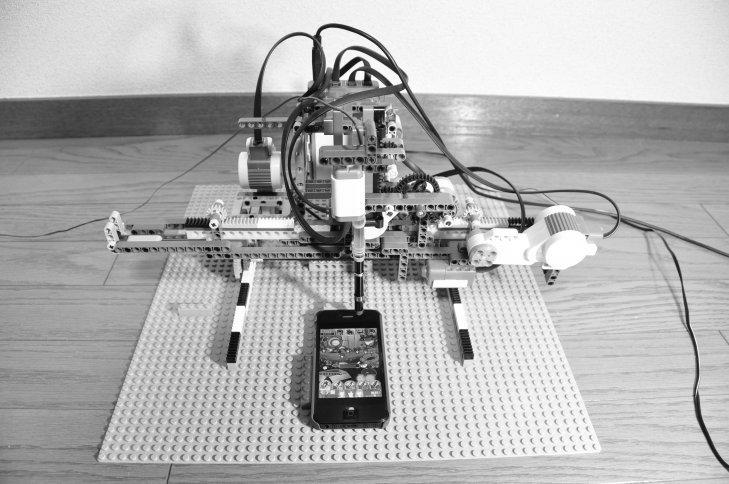
\includegraphics[width=0.7\hsize]{image201210/nxt-python_namekorobo2_mono.jpg}
  \end{center}
  \caption{なめこロボ}
  \label{fig:namekorobo2}
\end{figure}

\subsection{『なめこ栽培キット』とは}

原木になめこの餌を注入し、
生えてきたなめこを指でなぞって収穫するiPhoneおよびAndroidのゲームです。
株式会社ビーワークスからリリースされています。

\begin{itemize}
\item 正式名称は『おさわり探偵なめこ栽培キット』。
\item iPhone版での最新作は『おさわり探偵なめこ栽培キットDeluxe』。
\item たまにレアなめこが生える。
\end{itemize}

\subsection{レゴ マインドストームの紹介}

株式会社レゴが販売している教育用ロボットで、
次のような特徴を持っています。

\begin{itemize}
\item レゴブロックを使って組み立てられる
\item レゴ テクニックシリーズのパーツを使用する
\item モーターや各種センサーを制御できる
\item ARM7のコンピュータユニットから制御する
\item ETロボコンで使われている
\end{itemize}

\subsubsection{レゴ マインドストームの購入方法}
ETロボコンの委員をやっている先生に購入方法を伺ったところ、
「(株)アフレルから買ってください」と言われました。

\begin{itemize}
\item 教育用レゴ マインドストーム 正規代理店(株)アフレル
\item \url{http://www.afrel.co.jp/}
\item 現在価格 39,900円
\end{itemize}

こちらではETロボコン用のセット販売などを行っているようですが、
特にETロボコンにこだわらない場合、
Amazon.co.jpから現在価格34,000円で購入できます。

また一部のパーツは個別に購入することが可能です。
筆者は次のお店を利用しました。

\begin{itemize}
\item ホビーショップ デジラ \url{http://www.dgla.jp/shop/}
\item LEGOパーツ専門店 ハック フィン \url{http://huckfinn-lego.com/}
\item レゴ パーツ販売ショップ「ブリッカーズ」 \url{http://www.brickers.jp/}
\end{itemize}

マインドストームにはいくつか種類がありますが、
最新のものは『レゴ マインドストーム NXT 2.0』で、
筆者もこちらを購入しました。

\subsection{nxt-python}
今回の目的はなめこ栽培キットの自動収穫機であるため、
マインドストームを自立動作させる必要がありません。
nxt-pythonはPCとマインドストーム NXTをUSBやBluetoothで接続し、
PC側で実行したスクリプトに従ってマインドストームをコントロールするためのpythonモジュールです。

nxt-pythonは次の場所で公開されています。
\begin{itemize}
\item \url{http://code.google.com/p/nxt-python/}
\end{itemize}

Debian sidにはpython-nxtというパッケージがあり、
こちらを導入することでnxt-pythonが利用できます。

\begin{commandline}
$ sudo apt-get install python-nxt
\end{commandline}
%$

\subsubsection{サンプルコード}
次のコードはポートBに接続されたモーターをパワー100、
360度回転させるサンプルコードです。

\begin{commandline}
#!/usr/bin/python

import nxt.locator
from nxt.motor import *

b = nxt.locator.find_one_brick()
m_left = Motor(b, PORT_B)
m_left.turn(100, 360)
\end{commandline}

なおドキュメントは見つからなかったため、
ソースコードを読みながら使い方を調べました。

\subsubsection{BaseMotor::turn(power, tacho\_units)}

turn()はpowerにパワーを、tacho\_unitsに角度を指定してモーターを回すメソッドです。
\begin{itemize}
\item 回りきるまで制御は帰ってこない。
\item デフォルトでは回りきったところでブレーキをかける。
\item 途中でモーターが回転しなくなると例外を飛ばす。
\item powerは-100 $\sim$ 100を指定可能。
\item powerに負の値を指定すると回転が逆になる。
\item powerに-10 $\sim$ 10くらいの値を指定しても力が弱くてモーターは回らない。
\end{itemize}

\subsubsection{Motor::weak\_turn(power, tacho\_units)}
turn()は無理矢理モーターを手で止めると怪我をするくらい強く回しますが、
weak\_turn()はモーターを弱々しく回します。

\begin{itemize}
\item 手で止めると簡単にモーターは止まる。
\item このとき例外は飛ばさない。
\item 手で軽く回すと再び回り始める。
\item tacho\_units分回ると制御が帰る。
\item 使いどころが分からない。
\end{itemize}

\subsubsection{Motor::run(power=100)}

run()は指定されたパワーでモーターを回しつづけます。
run()を実行したのち、
制御はすぐに戻ってきます。
制御が戻ってきてもモーターは回りつづけます。

\subsubsection{Motor::brake(), Motor::idle()}
brake()およびidle()はモーターを止めるメソッドです。
brake()はモーターを止めて動かないようブレーキをかけますが、
idle()は惰性で回りつづけ、
緩やかに止まります。

\subsubsection{Motor::get\_tacho()}
モーターは何度回ったかをカウントしており、
get\_tacho()メソッドでこのカウンタを取得できます。
get\_tacho()は次のの三つの値を返します。
\begin{itemize}
\item .tacho\_count
\item .block\_tacho\_count
\item .rotation\_count
\end{itemize}

\subsubsection{Motor::reset\_position(relative)}
relativeにTrueを渡すと.block\_tacho\_countを、
Falseを渡すと.rotation\_countをリセットします。

\subsubsection{Touch::is\_pressed()}
タッチセンサーが押されていればTrueを、
それ以外はFalseを返します。

\subsubsection{その他}
turn()メソッドはデフォルトの動作でブレーキをかけてくれるのですが、
指定した数値どおりに動いてはくれません。
しかしtachoは正確な値に見えるので、
これを頼りに位置指定を行う関数を定義して利用しました。

\begin{commandline}
def absturn(m, p):
    d = 1
    c = m.get_tacho().rotation_count
    q = p - c
    if q &lt; 0:
        d = -1
        q = abs(q)
    m.turn(30*d, q)
\end{commandline}
% これ、HTMLエスケープっぽいけど本当に&lt;であってるの? --uekawa

\subsection{作成されたもの}

実際に動かしているコードをgistで公開しました。
\begin{itemize}
\item \url{https://gist.github.com/3897500}
\end{itemize}

動画はYouTubeで見られます。
\begin{itemize}
\item \url{http://www.youtube.com/watch?v=uIEyWBs68c8}
\item 「レゴ なめこ」で検索すると上の方に出てきます。
\end{itemize}

\subsection{最後に}
機械制御はなかなか思ったとおりに動いてくれないことが多く、
モーターが正確な位置に動いてくれないなどの苦労に見舞われましたが、
なんとか軽減することができました。

これを機会に皆さんもレゴ マインドストーム NXTの世界を覗いてみてはいかがでしょうか。

%-------------------------------------------------------------------------------
\dancersection{Android 携帯でBluetooth Tethering}{上川 純一}
%-------------------------------------------------------------------------------
\index{bluetooth}
\index{bluetooth tethering}
\index{tethering}

\subsection{はじめに}

最近のAndroid携帯もパソコンもBluetoothに対応しています。そしてBluetooth
profileであるPANやDUNに対応しているものも多いようです。
Android 4.0あたりで対応するようになったと思われるBluetooth Tetheringを利
用することでAndroid携帯にBluetooth PAN 経由で接続し、Android携帯の回線を
利用して外部のネットワークに接続できるようになります。

WiFi Tetheringのように電力消費が高すぎるので毎回設定でオフにする必要があ
るるということもなく、やUSB Tetheringのように毎回物理的に接続する必要もな
いので便利です。
カバンの中に携帯をいれたまま接続できるので気楽ですよ。

\subsection{設定方法}

Android携帯側ではBluetooth Tetheringをオンにします。

あと、Bluetoothのペアリングを行います。携帯電話側の設定で可視状態にして
おいてGNOMEの設定で追加すればよいでしょう。(\fgref{fig:gnome-bt2})

\begin{figure}[ht]
 \begin{center}
  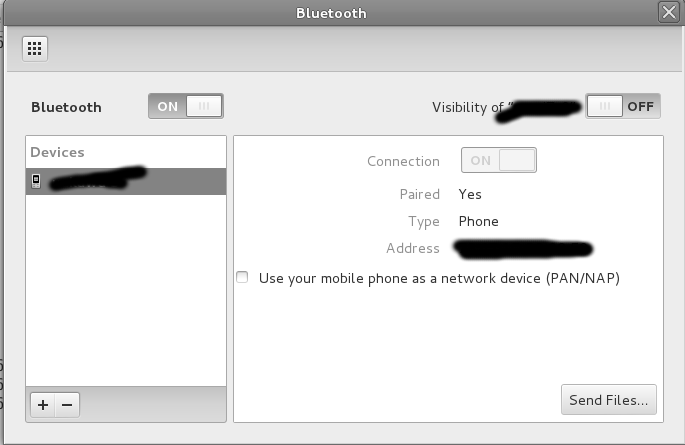
\includegraphics[width=0.5\hsize]{image201211/bt2_mono.png}
  \label{fig:gnome-bt2}
 \end{center}
\end{figure}

一旦設定しておくとネットワークの選択候補にMobile Broadbandというのが現れ
てそこで携帯電話のBluetooth PAN接続が選択できるようになります。

\begin{figure}[ht]
 \begin{center}
  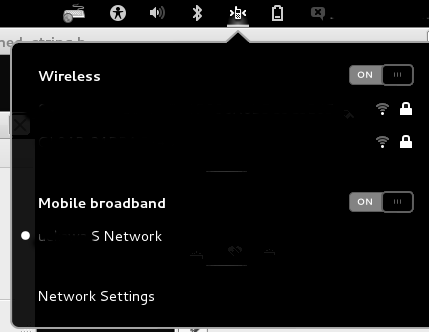
\includegraphics[width=0.5\hsize]{image201211/bt1_mono.png}
  \label{fig:gnome-bt1}
 \end{center}
\end{figure}

\subsection{ネットワーク構成}

Linux 側からはbnep0 デバイスとして見えます。複数マシンから接続するとそれ
ぞれが別のサブネットに接続されるっぽいのでお互いに通信はできないようです。
WiFi Tetheringだと同じサブネットにつながるので個人的にはウェブサーバーと
クライアントを接続するためのハブとして便利に利用していたのですが、そうい
う使い方はできないようです。

\begin{commandline}
bnep0     Link encap:Ethernet  HWaddr 
          inet addr:192.168.46.43  Bcast:192.168.46.255  Mask:255.255.255.0
\end{commandline}

\subsection{まとめ}

Bluetooth PANは便利、ということでした。ただ、なぜだか日本の携帯電話は
Bluetooth PANに対応してないものが多く、また海外携帯の日本モデルはその機能
を削ってたりするものがあります\footnote{例:筆者の所有するGalaxy Nexus
DoCoMo版}。ここはぜひBluetooth PAN対応じゃない携帯電話は購入しないことで
消費者の意見を表明してください。

%-------------------------------------------------------------------------------
\dancersection{perf でパフォーマンスチューニング}{上川 純一}
%-------------------------------------------------------------------------------
\index{perf}

\subsection{はじめに}

最近のたいていのCPUにはPerformance Counters という仕組みがあり、特定のイ
ベントが一定回数発生したらある処理をするという事ができるようになっていま
す。それを利用してプロファイラーが実装できて、プログラムのパフォーマンス
ボトルネックの発見に役立てることができます。
昔は oprofile を使っていたのですが、最近のLinux カーネルでは perf という
仕組みを使うのが主流のようです。

カーネル側のサポートは標準で入っています。コマンドラインの perf コマンド
は linux-base パッケージにはいっていてたいていの環境では標準でインストー
ルされているようにみえるのですが実体はカーネルにあったバージョンを追加で
インストールする必要があります。例えば、linux 3.2 だと linux-tools-3.2 を
インストールすることになります。

\begin{commandline}
 $ uname -r
3.2.0-3-amd64
 $ sudo apt-get install linux-tools-3.2
\end{commandline}
\index{linux-tools-3.2}

デバッグシンボルがあると関数名とかがきれいに出る気がするので利用している
ライブラリのデバッグシンボルもいれておくとよいでしょう。標準ライブラリは
いれておきましょう。

\begin{commandline}
 $ sudo apt-get install libc6-dbg libstdc++6-4.7-dbg
\end{commandline}
%$

\subsection{perf stat}

プログラム単体の実行時間を計測してレポートしてくれるコマンドとして timeコ
マンドがありますが、その代わりにつかえそうなツールとして、 perf stat があ
ります。最近のCPUは負荷によってCPU周波数が変わり、そういうシステムにおい
てパフォーマンスの測定のために実行時間だけを計測するというのは適切ではな
いのですが、perf statはそれ以外に必要そうな値を計測してくれるので便利です。

\begin{commandline}
$ perf stat ./apt-index-cmd debian_dists_sid_main_binary-amd64_Packages debian > /dev/null
 Performance counter stats for './apt-index-cmd debian_dists_sid_main_binary-amd64_Packages debian':

       1741.828818 task-clock                #    0.997 CPUs utilized          
               165 context-switches          #    0.000 M/sec                  
                 6 CPU-migrations            #    0.000 M/sec                  
            27,392 page-faults               #    0.016 M/sec                  
     4,990,934,326 cycles                    #    2.865 GHz                     [83.29%]
     1,681,297,382 stalled-cycles-frontend   #   33.69% frontend cycles idle    [83.27%]
     1,096,373,883 stalled-cycles-backend    #   21.97% backend  cycles idle    [66.62%]
     7,738,965,303 instructions              #    1.55  insns per cycle        
                                             #    0.22  stalled cycles per insn [83.51%]
     1,784,494,907 branches                  # 1024.495 M/sec                   [83.49%]
        32,701,183 branch-misses             #    1.83% of all branches         [83.32%]

       1.746581711 seconds time elapsed
\end{commandline}
  
\subsection{perf record}

perf record コマンドはプロファイル情報を記録する命令です。パラメータとし
て指定したコマンドをそのまま実行して、カレントディレクトリに perf.dataファ
イルを作成します。後に perf report などでそのプロファイルデータを確認する
ことができます。

\begin{commandline}
$ perf record ./apt-index-cmd debian_dists_sid_main_binary-amd64_Packages  debian > /dev/null
[ perf record: Woken up 1 times to write data ]
[ perf record: Captured and wrote 0.087 MB perf.data (~3800 samples) ]
$ ls -l perf.data
-rw------- 1 dancer dancer 93560 10月 10 07:03 perf.data

\end{commandline}

perf record -g オプションをつけるとコールグラフ情報も記録するようです。

デフォルトは一秒1000サンプルとるようなので、プログラムの実行時間に応じて
サンプル数を適当に調整しましょう。 例えば全体で実行が一秒で終わってしまう
プログラムの場合は-F 10000 をつけてみるとよりサンプル数がとれていいかもし
れません。

\subsubsection{gcc のコンパイルオプションの検討}

gcc でソースコードコンパイルするときに、-g オプションをつけるとデバッグ情
報がつきます。関数シンボルの情報とか行数とかソースコードとかが得られるの
でこれは多分重要。

コールグラフがあまりないなぁと思ったら最適化のしすぎとスタックトレースの
とりにくさを疑ってみましょう。

通常最適化オプション -O2 をつけてコンパイルしますが、amd64 の場合、gcc で
-O2 をつけてコンパイルするとフレームポインタがなくなってスタックトレース
を取得しにくくなっています。libunwind使えば取得できるはずですが、多分
perfはカーネル空間でスタックトレースをとっているのでそうなってないっぽい
です。対策として若干オーバーヘッドがありますが、-fno-omit-frame-pointer
を指定すると、フレームポインタを操作するコードを生成してくれます

C++でファンクションオブジェクトとかテンプレートプログラミングしまくってい
ると、関数がほとんどインライン展開されてしまい、コールグラフに現れる部分
が少なくなります。理解不能になってきたらたまに -O あたりでコンパイルして
スタックトレースを見てみましょう。

\subsection{perf report}

perf report コマンドは取得したプロファイルデータを可視化するコマンドです。
テキストコンソールメニュー形式になっていて、気になるシンボルを選択してソー
スコードのアノテーションを見ることができます。どのソースコードの行に対応
するアセンブラのどの命令でCPU処理時間を費やしたのかを表示してくれます。

\begin{commandline}
$ perf report
Events: 1K cycles                                                              
 18.65%  apt-index-cmd  apt-index-cmd        [.] available_parser::AptIndexSpiri
  7.38%  apt-index-cmd  libc-2.13.so         [.] _int_malloc
  6.64%  apt-index-cmd  libc-2.13.so         [.] malloc
  5.17%  apt-index-cmd  libstdc++.so.6.0.17  [.] std::string::_M_replace_aux(uns
  4.03%  apt-index-cmd  libc-2.13.so         [.] _int_free
  4.02%  apt-index-cmd  libstdc++.so.6.0.17  [.] __cxxabiv1::__vmi_class_type_in
  3.81%  apt-index-cmd  libstdc++.so.6.0.17  [.] std::string::_M_mutate(unsigned
  3.59%  apt-index-cmd  libstdc++.so.6.0.17  [.] std::ctype<char> const& std::us
  3.00%  apt-index-cmd  libc-2.13.so         [.] __strcmp_sse42
  2.74%  apt-index-cmd  apt-index-cmd        [.] boost::detail::function::functi
  2.72%  apt-index-cmd  libstdc++.so.6.0.17  [.] __dynamic_cast
  2.67%  apt-index-cmd  libc-2.13.so         [.] free
  2.46%  apt-index-cmd  libc-2.13.so         [.] __memcmp_sse4_1
\end{commandline}

ここでエンターをおすと次が表示され

\begin{commandline}

available_parser::AptIndexSpirited::MakeIndex()::{lambda(std::vector<char, std::
    0.00 :          40368a:       je     4036ac <available_parser::AptIndexSpir
         :                                                                     
         :          const std::string& get() const { return my_string_; }      
         :                                                                     
         :          // for 'map' comparison.                                   
         :          bool operator<(const OrderedHashedString& b) const {       
         :            if (ordered_hash_ == b.ordered_hash_) {                  
    2.87 :          40368c:       mov    0x28(%rbx),%rdx                       
         :              return my_string_ < b.my_string_;                      
         :            } else {                                                 
         :              return ordered_hash_ < b.ordered_hash_;                
   34.96 :          403690:       cmp    %rbp,%rdx                             
    1.43 :          403693:       setb   %cl                                   
         :                                                                     
         :          const std::string& get() const { return my_string_; }      
         :                                                                     
         :          // for 'map' comparison.                                   
         :          bool operator<(const OrderedHashedString& b) const {       
         :            if (ordered_hash_ == b.ordered_hash_) {                  
  
 \end{commandline}

\subsubsection{C++ のコードの場合}

C++でテンプレートを活用しているコードを眺める場合、perf report のTUIイン
タフェースだと関数名が十分表示されないなと悩むことになります。とりあえず
TUIじゃないインタフェースにするともっと表示されますが、いまいち全体は表示
できません。

たとえば関数名がこのように途中で切れてしまいます。まだ僕は回避方法を発見して
いません。

\begin{commandline}
 void
 MeasureRaw<std::unordered_map<boost::iterator_range<__gnu_cxx::__normal_iterator<char
 const*, std::string> >, int,
 RangeHash<boost::iterator_range<__gnu_cxx::__normal_iterator<char
 const*, std::string> > >,
 RangeEqualTo<boost::iterator_range<__gnu_cxx::__normal_iterator<char
 const*, std::string> > >,
 std::allocator<std::pair<boost::iterator_range<__gnu_cxx::__normal_iterator<char
 const*, std::string> > const, int> > >, __gnu_cxx::__normal_iterator
\end{commandline}

\subsubsection{おわりに}

一番基本的なPerfの使い方を紹介しました。sudo perf listの出力を確認すると
ハードウェアのいろいろなカウンタだけでなくカーネルが提供しているさまざま
なトレースポイントでのカウンタがあるのがわかります。どう使うか、夢は広が
りますね。

\begin{thebibliography}{98}
 \bibitem{perfman} perf(1) ``perf -- perfomance analysis tools for Linux''
	 manual page. perf\_{}3.2-report(1), etc.
\bibitem{perfwikitutorial} ``Tutorial -- Linux kernel profiling with
	perf'', 
	\url{https://perf.wiki.kernel.org/index.php/Tutorial}

\end{thebibliography}

%-------------------------------------------------------------------------------
\dancersection{systemd}{岩松 信洋}
%-------------------------------------------------------------------------------
\index{systemd}

\subsection{はじめに}
世の中の主要なLinuxディストリビューションは SysVinit の init scripts から
他のinit システムに移行しつつあります。
FedoraやArch Linuxがsystemd に移行を始めたということもあり、一部で盛り上がっている
(阿鼻叫喚ともいう)ようです。
まさか いまだに SysVinit を使っている Debian勉強会参加者がいるとは思えませんが、
盛り上がっているようなのでDebianとSystemdについてまとめてみました。

\subsection{systemdとは?}

RedHat に勤めている Lennart Poettering 氏によって開発されている init の代替プログラムです。
実際には init の代替だけではなく、Linux のサービス(デーモン)管理フレームワークとなっ
ています。
%Linux カーネル用のデバイス管理ツールである udev が systemd のソースにマージ
%されています。ログシステムもある。将来は cron や acpid などの代替え機能を
%提供する予定らしい。
今までのinitシステムの違いはサービスのプロセス管理を pid ではなく、cgroups を使う点と
サービスの起動をソケットとバスを使う点があります。これらは D-Bus を使って行います。これによってシステム立ち上げ処理をより並列的に行えるようになっています。
また、System V スタイルとBSDスタイルの両方をサポートしています。

開発は freedesktop.org
\url{http://cgit.freedesktop.org/systemd/systemd/}
で行われており、開発は活発で週に一度はバージョンアップしています。
最新バージョンは v195となっています。

\subsubsection{systemd の利点}
systemd は SysVinit と比べて次のような利点があります。

\begin{itemize}
\item 設定が容易。\\
SysVinit はシェルスクリプトで記述していたため、開発者によって書き方が異なります。
よって設定や内容の理解が難しいことがあります。systemd は設定方法や項目等が決まっているため、
設定しやすくなっています。

\item 起動が早い。 \\
シェルに依存していないのとデーモンが並列起動するため起動が早いです。

\item カーネルモジュールの操作、セッション管理、ログ管理、ディスクの暗号化などを
統合。

\end{itemize}

その他、作者による説明を\url{http://0pointer.de/blog/projects/why.html}から参照できます。

\subsection{Debianで使う}

systemd はもちろん Debian でも提供されており、testing / unstable で v44 が
利用できます。最新版とバージョンに差がありますが、アップストリームで
頻繁にバージョンアップするのでバージョンはあまり問題ではありません。
v44 でも systemd を十分に使うことができます。

いまのところ Debianに関する情報は \url{http://wiki.debian.org/systemd}
にまとまっていますが情報が少なく、内容も古いです。

\subsubsection{インストール}
先にも書いたように Debianでは v44 が最新版です。
apt-get / aptitude でインストールできます。

また、Linux カーネルは 2.6.39 以上、devtmpfs, fanotify, autofs4, cgroups が有効になっている
必要があります。

%\begin{commandline}
%$ uname -a 
%Linux debian 3.2.0-4-amd64 #1 SMP Debian 3.2.32-1 x86_64 GNU/Linux
%\end{commandline}
%$

インストールは以下のように実行します。

\begin{commandline}
$ sudo apt-get install systemd
\end{commandline}
%$

以下のパッケージが依存関係でインストールされます。
\begin{commandline}
libsystemd-daemon0
libsystemd-id128-0
libsystemd-journal0
libpam-systemd
\end{commandline}
%$

次に ブートローダにinit指定を追加します。grub を使っている場合、\texttt{/etc/default/grub} の\\
\texttt{GRUB\_CMDLINE\_LINUX\_DEFAULT} に {\bf init=/lib/systemd/systemd} を追記します。 

\begin{commandline}
変更前:
GRUB_CMDLINE_LINUX_DEFAULT="quiet"
変更後:
GRUB_CMDLINE_LINUX_DEFAULT="quiet init=/lib/systemd/systemd"
\end{commandline} 
%$

変更後、{\bf update-grub}を実行し、grub に設定を反映します。
そしてリブートします。
設定が間違っていないければ systemd で立ち上がるはずです。

\begin{commandline}
$ sudo update-grub
.....
$ sudo reboot 
\end{commandline}
%$

\subsubsection{起動速度}

systemd はアナライザをデフォルトでサポートしています。
起動にかかった時間を確認するには \texttt{systemd-analyze} を実行します。
また、画像で確認したい場合には \texttt{prop} オプションを指定して実行します。
SVG フォーマットで出力されるので、リダイレクトしてファイルに保存します。

\begin{commandline}
$ systemd-analyze 
Startup finished in 1831ms (kernel) + 5669ms (userspace) = 7500ms
$ systemd-analyze plot > systemd-boot.svg
\end{commandline}
%$

試しに自分が常用している環境で起動時間を測定したところ、
SysVinit は約15秒、systemd は約10秒でした。 

\subsection{用語}

systemd を扱っていると専門用語が出てきますので、説明します。

\begin{itemize}
\item ユニット\\
systemd ではデーモンなどの制御対象のことをユニットと呼びます。
ユニットにはサービス、デバイス、マウントポイントなど、いくつかの種類があります。
このユニットはテキストファイルで記述され、\texttt{/lib/systemd/system/} 以下に格納されています。
各ユニットは拡張子を持ち、サービスの場合は\texttt{.service}
となっています。


\begin{table}[htb]
\begin{center}
  \begin{tabular}{ll}
    ユニットの種類 & 説明 \\
    service & デーモン \\
    socket & ソケットによるデーモン \\
    target & multi-user.target \\
    device & udev で管理するデバイス \\
    snapshot & ある時点のinit の状態 \\
    timer & イベントから時間経過 \\
    path & 監視するパス \\
    mount & マウントポイント \\
    swap & スワップ \\
    automaount & 自動マウントポイント \\
  \end{tabular}
\caption{systemd で提供するユニット}
\label{tbl:unit}
\end{center}
\end{table}

mount, swap, automout は起動時に \texttt{/etc/fstab} から自動的に
ユニットを生成してくれます。

\item ターゲット\\
ターゲットとはSysVinit の runlevel 相当のものです。
これはディストリビューションによって異なります。
Debianの場合は以下のようになっています。

\begin{table}[htb]
\begin{center}
  \begin{tabular}{ll}
    run level & systemd のターゲット \\
    0 & poweroff.target \\
    1 & rescue.target \\
    2 - 5 & multi-user.target \\
    6 & reboot.target \\
  \end{tabular}
\caption{run levelとターゲットの対応}
\label{tbl:target}
\end{center}
\end{table}

この他にgraphical.target と emergency.target があります。
前者は X による起動を行うときに呼ばれるターゲット、後者は障害が起こった時に
起動できるようにするためのターゲットです。
ターゲットはカーネルのブートオプションに \texttt{systemd.unit=}で指定でき
ます。何も指定しない場合はdefault.target が呼ばれるようになっています。

\end{itemize}

\subsection{ユニットの操作方法}
systemd に移行した後、デーモン等の制御は /etc/init.d/ 以下を実行するのではなく、{\bf systemctl}
コマンドを使って操作します。以下にユニットの操作方法について説明します。
\index{systemctl}

\subsubsection{起動しているユニットを表示する}

起動しているユニットを表示するには sytemctl を実行します。

\begin{commandline}
$ systemct
...
console-setup.service     loaded active exited        LSB: Set console font and 
cron.service              loaded active running       LSB: Regular background pr
dbus.service              loaded active running       D-Bus System Message Bus
debian-fixup.service      loaded active exited        Various fixups to make sys
exim4.service             loaded active running       LSB: exim Mail Transport A
getty@tty1.service        loaded active running       Getty on tty1
ifup@eth0.service         loaded active exited        ifup for eth0
...
\end{commandline}
%$

\subsubsection{全てのユニットを表示する}

操作できるユニットを表示するには \texttt{--all} を指定します。
 
\begin{commandline}
$ systemctl --all
UNIT                      LOAD   ACTIVE   SUB       JOB DESCRIPTION
proc-sys...misc.automount loaded active   waiting       Arbitrary Executable Fil
dev-cdrom.device          loaded active   plugged       QEMU_DVD-ROM
dev-disk...QM00003.device loaded active   plugged       QEMU_DVD-ROM
dev-disk...QM00001.device loaded active   plugged       QEMU_HARDDISK
dev-disk...2dpart1.device loaded active   plugged       QEMU_HARDDISK
dev-disk...2dpart2.device loaded active   plugged       QEMU_HARDDISK
...
\end{commandline}
%$

\subsubsection{ユニットの状態を確認する}

ユニットの状態を確認するには、\texttt{status} オプションに確認したいユニット名を
指定して実行します。

以下に rsyslog.service ユニットの状態を確認する例を示します。
\begin{commandline}
$ systemctl status rsyslog.service
    Loaded: loaded (/lib/systemd/system/rsyslog.service; enabled)
    Active: active (running) since Wed, 14 Nov 2012 00:37:18 -0800; 22h ago
   Process: 474 ExecStartPre=/bin/systemctl stop systemd-kmsg-syslogd.service (code=exited, status=0/SUCCESS)
  Main PID: 483 (rsyslogd)
    CGroup: name=systemd:/system/rsyslog.service
           └ 483 /usr/sbin/rsyslogd -n -c5
\end{commandline}
%$

これにより、このユニットは \texttt{/lib/systemd/system/rsyslog.service}によって
\texttt{Wed, 14 Nov 2012 00:37:18 -0800}に起動していることが分かります。

\subsubsection{ユニットを起動する}

起動していないユニットを起動するには、 \texttt{start}オプションにユニット名を指定して実行します。
これは \texttt{/etc/init.d/サービス start}と同様の動きとなります。
\begin{commandline}
$ sudo systemctl start ユニット名
\end{commandline}
%$

\subsubsection{ユニットを停止する}

起動しているユニットを停止するには、\texttt{stop}オプションにユニット名を指定して実行します。
これは \texttt{/etc/init.d/サービス stop}と同様の動きとなります。
\begin{commandline}
$ sudo systemctl stop ユニット名
\end{commandline}
%$

\subsubsection{ユニットの設定を再読み込みする}

ユニットの設定を再読み込みするには、\texttt{daemon-reload}オプションにユニット名を指定して実行します。
\begin{commandline}
$ sudo systemctl daemon-reload ユニット名
\end{commandline}
%$

実際に動いているデーモンの設定、例えばhttpdの設定を再読み込みし、再起動するには \texttt{reload}オプションを使います。

\subsubsection{ユニットの自動起動を有効にする}

ユニットの自動起動を有効にするには \texttt{enable} オプションにユニット名を指定して実行します。

有効にすると \texttt{/etc/systemd/system/ターゲット.wants/}に\texttt{/lib/systemd/system/}にあるユニット
へのシンボリックリンクが作成されます。
どのターゲットで自動起動が有効になるかは、ユニットファイルの \texttt{Install}セクションで指定します。

\begin{commandline}
$ sudo systemctl enable ユニット名
\end{commandline}
%$

\subsubsection{ユニットの自動起動を無効にする}

ユニットの自動起動を無効にするには \texttt{disable} オプションにユニット名を指定して実行します。
無効にすると、/etc/systemd/system/ターゲット.wants/にあるシンボリックリンクが削除されます。

\begin{commandline}
$ sudo systemctl disabe ユニット名
\end{commandline}
%$

\subsubsection{ユニットの詳細を確認する}

ユニットの詳細を確認するには \texttt{show} オプションにユニット名を指定して実行します。
これにより指定したユニットと他のユニット、ターゲットの関係などが分かります。

\begin{commandline}
$ sudo systemctl show rsyslog.service
Id=rsyslog.service
Names=syslog.service rsyslog.service
Requires=basic.target
Wants=syslog.socket
WantedBy=multi-user.target
Conflicts=shutdown.target
...                                                           
\end{commandline}                                                                                    
%$

\subsection{ユニットについて}
ユニットには各ユニット間の依存関係を記述することができます。
依存関係の指定として以下があります。

\begin{table}[htb]
\begin{center}
  \begin{tabular}{ll}
    定義 & 説明 \\
    Before & そのユニットの後に起動されるべきユニット。 \\
    After & そのユニットの前に起動されるべきユニット。 \\
    Conflicts & 同時に起動できないユニット。 \\
    Service & ソケットによる起動を行うユニット。 \\
    Sockets & ソケットによるユニットの起動を行う場合のソケット情報 \\
    Wants  & 同時に起動してほしいユニット。成功、失敗は関係ない。\\
    Requires & 同時に起動されなければならないユニット。ユニットの起動が失敗した場合は要求元も失敗する \\
    BindTo & ユニットをグループとしてまとめる。
%ユニットがなくなった場合、グループで指定されているユニットは停止される。\\
  \end{tabular}
\caption{ユニットの依存定義}
\label{tbl:unit-depends}
\end{center}
\end{table}

例えば、default.target の内容は以下のようになっています。
\begin{commandline}
[Unit]
Description=Graphical Interface
Requires=multi-user.target
After=multi-user.target
Conflicts=rescue.target
AllowIsolate=yes
\end{commandline}

このターゲットは
multi-user.targetと同時に起動され、multi-user.targetの後に起動します。
また、rescue.targetと同時に起動できません。

\subsection{まとめ}

Debian でも問題なくsystemd が利用できる環境が整っています。
レガシーなSysVinitは捨て、新しいinitの世界へ足を踏み入れてみてはいかがでしょうか。

\subsection{参考文献}
\url{http://www.slideshare.net/moriwaka/systemd}

%-------------------------------------------------------------------------------
\dancersection{Debian で作る LDAP サーバ}{佐々木 洋平}
%-------------------------------------------------------------------------------
\index{ldap}

\subsection{はじめに}

京都に来てから最初にやった業務は\texttt{Solaris8}と\texttt{NIS}の撲滅でし
た。特に複雑な要件は無かったのでOpenLDAPに移行して、ここ数年は順調に動作
して(いると思って)います。

$\cdots$で、気がついたら手元の仮想マシン群(各種Linuxディストリビューショ
ン、FreeBSD、Windows7など)の認証も、ホストOS(Debian)のOpenLDAPで行なうよ
うになっていました。ラップトップで常に\texttt{slapd}を上げているのもなん
かアレですが、気にしたら負けです。

とういわけで、ここでは「DebianでOpenLDAPサーバ(\texttt{slapd})を動かして、
色んなユーザ認証を一本化するまで」のお話をしてみたいと思います。
%
ちなみに、この企画を思いついた理由は「ネット上にある多くのドキュメントが
古い\texttt{slapd}について書かれていて、実際に運用しようとしたら色々とハ
マったから」だったんですが、先日倉敷さんに「Ubuntu Server Guide読んでねー
のかよ(ry」とバッサリ言われてしまいました。$\cdots$で読んでみたら、記事を
書く気力が $\cdots$。

気をとりなおして、先に進みます。

\subsection{LDAP:Lightweight Directory Access Protocol}

LDAP はディレクトリサービス(正確には X.500 モデルをサポートするディレクト
リサービス)に接続するために使用するためのプロトコルの一つです。ここでの
「ディレクトリ」はファイルを管理する階層構造ではなくて、「住所氏名録、人
名簿」の意味でのディレクトリです。X.500 データモデルはデータ構造(X.500)、
認証(X.509)、分散処理(X.518)、複製(X.525)といった標準規格と、これらにアク
セスするためのプロトコルである DAP: Directory Access Protocol があります。
この DAP を軽量化し、TCP/IP の上で実装したのが LDAP です。

\subsection{DIT: Directory Information Tree}

LDAPがアクセスするディレクトリデータは「住所録・名簿」であり、「人」や
「物」及びこれらに付随する情報(パスワードやメールアドレスなど)を管理する
ことに特化しています。これらの情報は頻繁に参照されることはあっても、更新
はさほど行なわれません。この点は MySQL などのリレーショナルデータベースと
異なる点です。

LDAP のアクセスするデータベースは「木構造」になっています。この木構造
を DIT と呼びます。DIT の各ノードは「エントリ」と呼ばれ、これらエントリに
は rdn: Relative Distinguished Name(相対識別名)が付いています。rdn をつな
げることで、エントリの dn:Distinguished Name(識別名)が一意に定まり、DIT
中で識別されます。ひとつのエントリには「属性名」と「属性値」がペアとなっ
て幾つか格納されています。属性名と属性値のテンプレートが objectClass です。
図(\ref{fig:DIT})に、DIT の例を示します。この例で
は、\texttt{localhost.localdomain}上で objectClass として \texttt{person} を用いて、
アカウント名とパスワードによる認証情報が格納されています。
\begin{figure}[h!]
  \begin{tabular}{cc}
    \begin{minipage}{0.38\linewidth}
      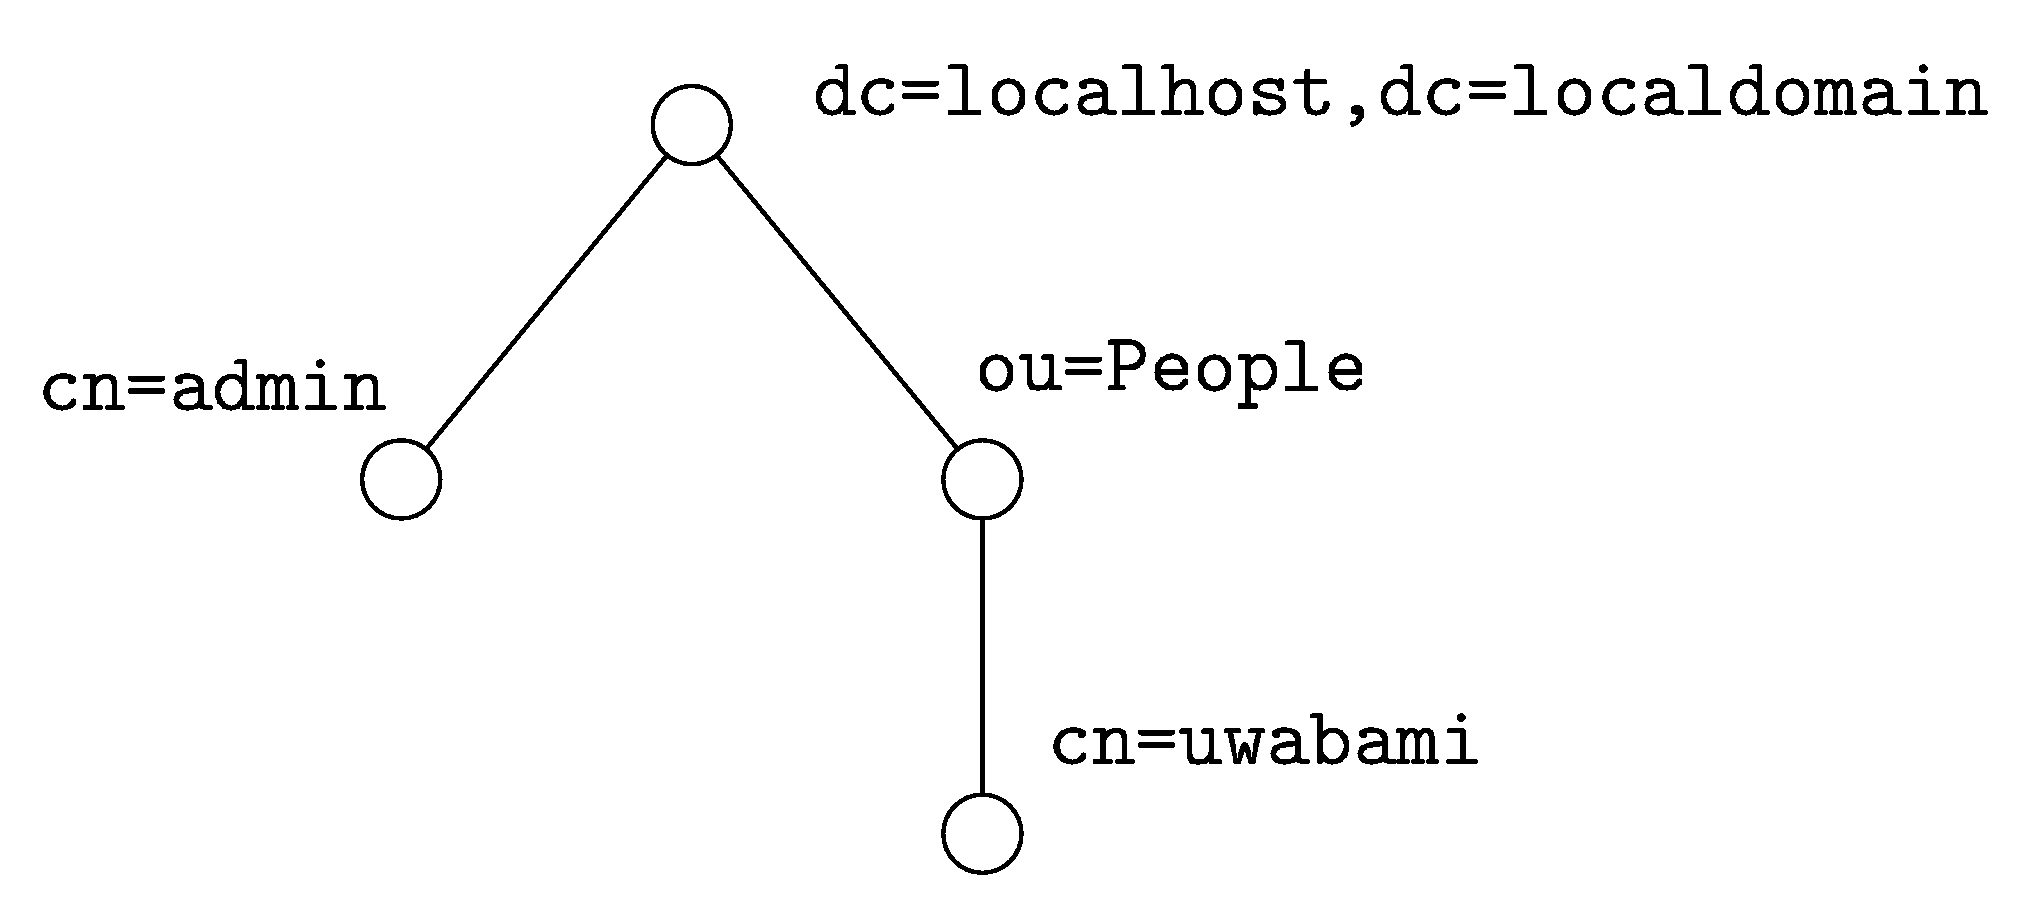
\includegraphics[width=.98\linewidth]{image201207/ldap-node-example.png}
    \end{minipage}
    \begin{minipage}{0.6\linewidth}
      \vspace{3em}
      \begin{screen}
        {\small
        \texttt{cn=uwabami,ou=People,dc=localhost,dc=localdomain}
        \begin{tabular}{ll}
          \texttt{objectClass}:
          & \texttt{person}                                 \\
          \texttt{cn}:
          & \texttt{Youhei SASAKI}                          \\
          \texttt{sn}:
          & \texttt{SASAKI}                                 \\
          \texttt{userPassword}:
          & \texttt{\{SSHA\}jP68h6yzJOlnRMda7IFI0LrTSe/lrFgO} \\
          $\cdots$ &\\
        \end{tabular}
        }
      \end{screen}
    \end{minipage}
  \end{tabular}
  \caption{DITの例。この場合
    の rootdn は \texttt{dc=localhost,dc=localdomain}となり、一番右下のエ
    ントリの dn は \texttt{cn=uwabami,ou=People,dc=localhost,dc=localdomain}と
    なる。}
  \label{fig:DIT}
\end{figure}

DIT中のエントリにどの様な情報を格納するのか、というスキーマ
は objectClass の集りであり、代表的な用途に用いられるスキーマは既に提供さ
れています。また、必要な情報を独自に定義して、新たに格納することも可能です。

\subsection{OpenLDAPの導入と初期設定}

LDAP サーバを導入して試してみます。Debianでは OpenLDAP サーバ
は \texttt{slapd} としてパッケージ化されていますので、これを導入します。
%
とりあえずラップトップの母艦と仮想マシン上の複数のクライアントを想定しますので
\begin{center}
  \texttt{rootdn: dc=vmhost,dc=localdomain}
\end{center}
で設定を始めてみます。

先ずは名前解決ができるようにしておきます。
自前で DNS を上げているのであれば問題無いのですが、
そうではない場合に備えて /etc/hosts あたりに
\begin{commandline}
  127.0.1.1     vmhost.localdomain vmhost
\end{commandline}
などと追記して
\texttt{dig}や\texttt{nslookup}で名前解決ができることを確認しておきます.
%
続いてインストールです。
\begin{commandline}
  $ sudo -s
  # apt-get install slapd ldap-utils
\end{commandline}
%$
debconf の dialog が出てくるので適宜答えると良いでしょう。
\begin{enumerate}
\item Omit OpenLDAP server configuration?
  → No
\item DNS domain name:
  → vmhost.localdomain
\item Organization name:
  → localdomain
\item Administrator password:
  → 適宜
\item Database backend to use: BDB でも HDB でもお好きな方を.
  HDB は subtree の rename をサポートしている。
\item Do you want to the database to be removed when slapd is purged?
  → Yes
\item Allow LDAPv2 protocol?
  → No
\end{enumerate}
この状態で、LDAP のデータベースには二つの DIT が存在します。
一つ目は管理用の DIT、二つ目はサービス用のデータを入れていく DIT です。
それぞれ以下で確認できます。
\begin{commandline}
$ sudo ldapsearch -Q -LLL -Y EXTERNAL -H ldapi:/// -b cn=config dn
dn: cn=config

dn: cn=module{0},cn=config

dn: cn=schema,cn=config

dn: cn={0}core,cn=schema,cn=config

dn: cn={1}cosine,cn=schema,cn=config

dn: cn={2}nis,cn=schema,cn=config

dn: cn={3}inetorgperson,cn=schema,cn=config

dn: olcBackend={0}hdb,cn=config

dn: olcDatabase={-1}frontend,cn=config

dn: olcDatabase={0}config,cn=config

dn: olcDatabase={1}hdb,cn=config

$ sudo ldapsearch -x -LLL -H ldap:/// -b dc=vmhost,dc=localdomain dn
dn: dc=vmhost,dc=localdomain

dn: cn=admin,dc=vmhost,dc=localdomain
\end{commandline}

では次に、ユーザ認証/管理ができるようにしてみます。
/etc/{passwd,shadow,groups} 相当のスキーマとして、
\begin{itemize}
\item \texttt{ou=People,dc=vmhost,dc=localdomain}というエントリ以下にユーザを格納
\item \texttt{ou=Groups,dc=vmhost,dc=localdomain}というエントリ以下にグループを格納
\item \texttt{cn=uwabami,ou=Groups,dc=vmhost,dc=localdomain}というグループを追加
\item \texttt{cn=uwabami,ou=People,dc=vmhost,dc=localdomain}というユーザを追加
\end{itemize}
する LDIF(LDAP Data Interchange Format)ファイルを書き, ldapadd で DIT に追加します。
\begin{commandline}
  $ cat add_People.ldif
  #
  # ユーザを格納するエントリの追加
  #
  dn: ou=People,dc=vmhost,dc=localdomain
  objectClass: organizationalUnit
  ou: People

  $ cat add_Groups.ldif
  #
  # Groups を格納するエントリの追加
  #
  dn: ou=Groups,dc=vmhost,dc=localdomain
  objectClass: organizationalUnit
  ou: Groups

  $ cat add_account_uwabami.ldif
  dn: cn=uwabami,ou=Groups,dc=vmhost,dc=localdomain
  objectClass: posixGroup
  cn: uwabami
  gidNumber: 3000

  dn: uid=uwabami,ou=People,dc=vmhost,dc=localdomain
  objectClass: inetOrgPerson
  objectClass: posixAccount
  objectClass: shadowAccount
  uid: uwabami
  sn: SASAKI
  givenName: Youhei
  cn: Youhei SASAKI
  displayName: Youhei SASAKI
  uidNumber: 3000
  gidNumber: 3000
  userPassword: {SSHA}jP68h6yzJOlnRMda7IFI0LrTSe/lrFgO
  gecos: Youhei SASAKI, admin of this computer.
  loginShell: /bin/zsh
  homeDirectory: /home/uwabami
\end{commandline}
%$
LDIF ファイルの形式は
\begin{itemize}
\item 属性名: 属性値
\item 継続行の先頭は空白
\item 行頭の \# 以降はコメント扱い。空白行は無視
\end{itemize}
です。また、パスワードは \texttt{slappasswd} コマンドで
ハッシュにしておきます。
\begin{commandline}
  $ slappasswd -h {SSHA} -s OpenSeSaMi
  {SSHA}jP68h6yzJOlnRMda7IFI0LrTSe/lrFgO
\end{commandline}
%$
注意したいのは uid/gid の数値です。Debianでは一般ユーザは1000番台から始まります。
ファイルで管理されている/追加されるユーザやグループと被らないように、ここでは 3000 番にしました。

LDIF ファイルを書いたら、この内容を実際に追加します。
\begin{commandline}
  $ ldapadd -x -D cn=admin,dc=vmhost,dc=localdomain -W -f add_People.ldif
  Enter LDAP Password:
  adding new entry "ou=People,dc=daphne,dc=localdomain"
  ...
\end{commandline}
%$
と出れば成功です。 実際にユーザやグループ作成されたか検索してみます
\begin{commandline}
  $ ldapsearch -x -LLL -b dc=vmhost,dc=localdomain 'uid=uwabami' cn gidNumber
  dn: uid=uwabami,ou=People,dc=vmguest,dc=localdomain
  cn: Youhei SASAKI
  gidNumber: 3000
\end{commandline}
%$
どうやらうまく追加できたようです。

\subsection{Linuxクライアントのユーザ認証}

単なるユーザ認証系として使用するのであれば、
Ubuntu ($>$=12.04) や Debian (squeeze 以降) で
\begin{itemize}
\item \texttt{libnss-ldapd}
\item \texttt{libpam-ldapd}
\item \texttt{nscld}
\end{itemize}
を導入し、debconf の質問に適宜答えるだけでおしまいです.
\begin{commandline}
  $ sudo -s
  # apt-get install libnss-ldapd libpam-ldapd nslcd
\end{commandline}
%$
\begin{itemize}
\item LDAPサーバの URI→適宜
\item LDAPサーバの検索を開始する DN → dc=vmhost,dc=localdomain
\item nsswitch の更新: 設定する名前サービスとして passwd, group, shadow を選択
\end{itemize}
前半二つは nslcd の設定です。
通常の debconf のダイアログでは、ユーザ認証に関する事柄を聞かれないので
\begin{commandline}
  $ sudo dpkg-reconfigure -plow nslcd
\end{commandline}
%$
として、rootbinddn や rootpw を設定しておきます。

\texttt{finger} や \texttt{id} などで、
先程追加したユーザが見えることを確認した後、ログインを試してみる良いでしょう。

\subsection{まとめ}

というわけで、とりあえず OpenLDAP を用いてユーザ認証を統合するまで、
について走り書きですがまとめてみました。
実際には
\begin{itemize}
\item slapd のアクセス制限、DIT の ACL とか STARTTLS
\item インデックス生成によるデータベースの高速化や複製/多重化
\end{itemize}
なんて話題もありますので、これについては発表の時に補足します。
次回はこれらに付け加えて
Samba と連携した NT ドメインの管理なんかについてまとめてみるつもりです。

%-------------------------------------------------------------------------------
\dancersection{Debian ではじめる Kerberos 認証}{倉敷 悟}
%-------------------------------------------------------------------------------
\index{kerberos}
\subsection{事前課題の確認}

今回の事前課題は、「MIT 版 Kerberos のサービスを構成するプロセスと、そのプロセスが使用するポートを 2 つ以上挙げてください」でした。

正解は、MIT 版 Kerberos の管理ガイド\footnote{\url{http://web.mit.edu/kerberos/krb5-1.10/krb5-1.10.3/doc/krb5-admin.html}\\
\#Configuring-Your-Firewall-to-Work-With-Kerberos-V5}を参照してください。一応、Kerberos 化されたサービスなどを省いた模範回答例は下記の通りです。

\begin{description}
\item [krb5kdc] 88/tcp,udp
\item [kadmind] 749/tcp
\item [kpropd] 754/tcp
\end{description}

\subsection{kerberos とは}

1980 年代に MIT のアテナプロジェクト\footnote{興味のある方は、「MITアテナプロジェクトのすべて」という書籍を読むと楽しめる思います}で (X Window System などとともに) 開発された、オープンなネットワークにおける認証システムです。もともと、MIT のオープンキャンパスにおける課題を解決するために開発されているため、セキュアではない分散環境での動作が前提になっている他、シングル・サインオンもサポートされています。

開発初期に公開するうえで米国の暗号政策 (輸出禁止) を回避する必要があったため、kerberos には複数の実装があります。ただ、現在では特に問題なく MIT の実装を利用することができますので、別実装のことはひとまずおいておきましょう。興味のある方は kth とか heimdal とかでググってみてください。

バージョン5以降では、kerberos プロトコルとして RFC が発行されています\footnote{http://www.ipa.go.jp/security/rfc/RFC.html\#10}。また、Windows2000 以降の AD 認証でも利用されているので、気付かないうちに使っていた、という方もいるかもしれません。

\subsubsection{kerberos の用語}

\begin{description}
  \item [レルム] ある KDC が管理対象とするネットワークの範囲です。DNS ドメインと対応させることが多いようです。ActiveDirectory 的にはフォレストになります。
  \item [プリンシパル] kerberos の管理対象となるあらゆる個別の要素です。ユーザ、ホスト、サービスなどが含まれます。次の書式の文字列で表現されます。「名前/識別子@レルム」

  \item [鍵発行局 (KDC: Key Distribution Center)] kerberos のキモとなるサービスです。管理レルムに所属している全プリンシパルの秘密鍵を保持しており、ユーザの認証 (AS) と、チケットの発行 (TGS) を行います。

  \item [チケット] ユーザからの要求に応じて鍵発行局で生成される、期限つきの認証データで、共有鍵で暗号化されています。

  \item [TGT (Ticket Granting Ticket)] ユーザが認証に成功した場合に発行されるチケットで、内部に一時的なセッション鍵を保持しています。これを持っているユーザのみ、サービスチケットの発行が許可されます。
  \item [鍵テーブル (Key Table)] Kerberos 認証を受けるサービスで必要となる、プリンシパルと鍵の一覧ファイルです。KDC 上でホストプリンシパルとサービスプリンシパルを作成し、それをファイルに出力してから該当のホストにコピーする必要があります。

\end{description}

Kerberos の仕組みや動作の詳細については、「3分間 NetWorking」というサイト\footnote{\url{http://www5e.biglobe.ne.jp/\%257Eaji/3min/ex/sup04.html}}が語り口も軽く、わかりやすいと思いますので一度読んでみてください。20 分ほどで読めます。

\subsection{構成の事前準備}
kerberos では、ホストの名前解決ができること、時刻が同期していること、が前提条件として必要になります。ちょっと面倒ですが、確認しておいてください。

適当な仮想化機能を使った実験であれば、名前解決は dnsmasq パッケージを導入して /etc/hosts にさっくり書くのがお手軽で便利かと思います。

\subsection{認証サーバの構成}

\subsubsection{openldap}
ユーザ認証の観点では、kerberos はアカウント名とパスワードの組だけを扱いますので、ホームディレクトリやシェルが設定できません。そこで今回は、openldap をアカウントのメタデータを保管するデータベースとして使用します。
openldap の構築と設定については、佐々木さんによる前回の関西 Debian 勉強会資料か、同じく佐々木さんによる次回の Debian 勉強会資料を参考にしてください。ここでは、すでに設定が完了しているものとして進めます。

/etc/passwd と /etc/shadow 相当のデータを保持するものとして、オブジェクトクラスは posixAccount と shadowAccount を利用します。ただし、実際には shadowAccount の属性は利用しません。
/etc/shadow 相当の実データは kerberos で取り扱うのですが、それは OS から shadow 情報として見えるわけではないので、フェイクのアクセス先という位置付けです。

\subsubsection{kerberos}

まずは kerberos サービス用のパッケージをインストールしてみましょう。インストールするホストの名前を krbtest.my.domain とすると、次のような構成となります (openldap と kerberos は 1 台のサーバに同居させる想定)。

\begin{table}[htb]
  \begin{tabular}{lcccr}
    クライアント & LDAP & Kerberos & TLS & 備考 \\

    レルム & MY.DOMAIN \\
    Kerberos (鍵発行局) サーバ & testnode.my.domain \\
    Kerberos 管理サーバ & testnode.my.domain \\
    openldap サーバ & testnode.my.domain \\
  \end{tabular}
\end{table}


\begin{commandline}
unset DEBIAN_FRONTEND ※pbuilder で実験している場合
apt-get install lv vim
apt-get install krb5-kdc krb5-admin-server
\end{commandline}

krb5-kdc が鍵発行局で、krb5-admin-server がアカウント情報の管理プロトコルを処理します。debconf がいくつか質問をしてくると思いますが、「Yes/No の質問は全てデフォルト通り」、「Default Kerberos version 5 realm」には名前解決で使っているドメイン名、「サーバアドレス」には名前解決できるホスト名、をそれぞれ入力してください。

kerberos 全般の設定ファイルは、/etc/krb5.conf になります。インストール時に debconf が自動で生成してくれるのですが、変更が不足しているので手編集が必要です。

\begin{commandline}
vi /etc/krb5.conf
\end{commandline}

\begin{itemize}
\item (必須) [domain\_realm]にドメインの設定を追加
\item (オプション) [realms] から不要なものを消す
\item (オプション) [domain\_realm] から不要なものを消す
\end{itemize}

設定ファイルの編集が終わったら、kerberos のデータベースを初期化しましょう。debian には、このためのちょっとしたスクリプトが付属しています。

\begin{commandline}
krb5_newrealm
\end{commandline}

root/admin のパスワードを求められますので、入力してください。これを忘れるとどうにもならなくなるので、忘れないように別途しっかり管理しておきましょう。
この段階で、空のデータベースが作成され、krb5-kdc (と kadmind) が起動され、各種プリンシパルの登録や変更ができるようになっています。

\subsection{データの登録}

\subsubsection{kadmin.local}

kerberos の管理作業に使うコマンドには、kadmin、kadmin.local、kdb5\_util などがあります。このうち、kadmin.local は管理サーバ上でのみ利用できるものです。
kadmin を使うには kerberos でのユーザ認証をパスする必要がある、つまりプリンシパルを登録してからでないと使えないので、最初は kadmin.local で管理作業を行います。

kadmin.local を実行すると、プロンプトが出力されて管理コマンドの入力待ちになります。'?' でコマンドのリストが表示されますので眺めてみましょう。

\begin{commandline}
kadmin.local:  ?
Available kadmin.local requests:

add_principal, addprinc, ank
                         Add principal
delete_principal, delprinc
                         Delete principal
modify_principal, modprinc
                         Modify principal
rename_principal, renprinc
                         Rename principal
change_password, cpw     Change password
get_principal, getprinc  Get principal
list_principals, listprincs, get_principals, getprincs
                         List principals
add_policy, addpol       Add policy
modify_policy, modpol    Modify policy
delete_policy, delpol    Delete policy
get_policy, getpol       Get policy
list_policies, listpols, get_policies, getpols
                         List policies
get_privs, getprivs      Get privileges
ktadd, xst               Add entry(s) to a keytab
ktremove, ktrem          Remove entry(s) from a keytab
lock                     Lock database exclusively (use with extreme caution!)
unlock                   Release exclusive database lock
purgekeys                Purge previously retained old keys from a principal
get_strings, getstrs     Show string attributes on a principal
set_string, setstr       Set a string attribute on a principal
del_string, delstr       Delete a string attribute on a principal
list_requests, lr, ?     List available requests.
quit, exit, q            Exit program.
\end{commandline}

とりあえず、ここではプリンシパルの登録と確認だけざっくり見てみることにします。

\subsubsection{ユーザプリンシパル}

ユーザの追加は簡単で、プリンシパルの名前としてユーザ名を指定するだけです。パスワードを求められますので、入力してください。

\begin{commandline}
kadmin.local:  addprinc kdmtest
WARNING: no policy specified for kdmtest@MY.DOMAIN; defaulting to no policy
Enter password for principal "kdmtest@MY.DOMAIN":
Re-enter password for principal "kdmtest@MY.DOMAIN":
Principal "kdmtest@MY.DOMAIN" created.
\end{commandline}

\subsubsection{ホストプリンシパル}

ホストを追加する場合は、プリンシパルの名前として host、識別子としてそのホストの FQDN を指定します。
また、ホストの場合はパスワードを人間が入力することはないので、手入力でなくランダムなものを自動生成させます。

\begin{commandline}
kadmin.local:  addprinc -randkey host/testnode.my.domain
WARNING: no policy specified for host/testnode.my.domain@MY.DOMAIN; defaulting to no policy
Principal "host/testnode.my.domain@MY.DOMAIN" created.
\end{commandline}

\subsubsection{サービスプリンシパル}

サービスを追加する場合は、プリンシパルの名前としてサービス名、識別子としてサービスを提供するホストの FQDN を指定します。

\begin{commandline}
kadmin.local:  addprinc -randkey ldap/testnode.my.domain
WARNING: no policy specified for ldap/testnode.my.domain@MY.DOMAIN; defaulting to no policy
Principal "ldap/testnode.my.domain@MY.DOMAIN" created.
\end{commandline}

\subsubsection{登録データの確認}

listprincs コマンドで、登録されているプリンシパルの一覧を表示することができます。初期状態では、次のように表示されるはずです。

\begin{commandline}
kadmin.local:  listprincs
K/M@MY.DOMAIN
kadmin/admin@MY.DOMAIN
kadmin/changepw@MY.DOMAIN
kadmin/testnode.my.domain@MY.DOMAIN
krbtgt/MY.DOMAIN@MY.DOMAIN
\end{commandline}

\subsubsection{鍵テーブルファイル (ktab) の生成}

プリンシパル名を指定して ktadd コマンドを実行することで、鍵テーブルを作成/更新することができます。
特定サービスホスト用の鍵テーブルファイルは、面倒ですが別途転送しておく必要がありますので、忘れないように注意しましょう。

\begin{commandline}
kadmin.local:  ktadd ldap/testnode.my.domain
Entry for principal ldap/testnode.my.domain with kvno 2, encryption type aes256-cts-hmac-sha1-96 added to keytab
FILE:/etc/krb5.keytab.
Entry for principal ldap/testnode.my.domain with kvno 2, encryption type arcfour-hmac added to keytab FILE:/etc/krb5.keytab.
Entry for principal ldap/testnode.my.domain with kvno 2, encryption type des3-cbc-sha1 added to keytab FILE:/etc/krb5.keytab.
Entry for principal ldap/testnode.my.domain with kvno 2, encryption type des-cbc-crc added to keytab FILE:/etc/krb5.keytab.
\end{commandline}

\subsection{クライアントの構成}

NSS に参照させるライブラリには、いくつかの選択肢が存在します。

\begin{table}[htb]
  \begin{tabular}{lcccr}
    クライアント & LDAP & Kerberos & TLS & 備考 \\
    lib(nss/pam)-ldap & ○ & × & 未対応 & 古いが多機能 \\
    lib(nss/pam)-ldapd & ○ & × & 対応 & squeeze 以降の推奨。まだ発展途上 \\
    libpam-krb5 & × & ○ & − & \\
    sssd & ○ & ○ & 必須 & RedHat が FreeIPA のために開発している。まだ発展途上 \\
  \end{tabular}
\end{table}

Debian 的には、今回の構成であれば libnss-ldapd + libpam-krb5 が本命ということになるのかも知れませんが、ここでは試しに sssd を使ってみることにします。

sssd は、RedHat がよくやる、あれこれ一緒くたにまとめる系の再実装の一つです。上記の ldap/krb 向けのクライアント機能の他、NSCD の機能も持っています。

\subsubsection{sssd の構成}

sssd は RHEL5 から登場し、RHEL6 でさらに統合が進んでいる他、日本語のマニュアルもきっちり用意されていますので、RedHat を使用している人には今後の標準となっていくであろうサービスです。

Debian にもパッケージはあるのですが、当然ながら RHEL に収録されているものとはバージョンが異なりますので、RedHat のマニュアルをそのまま使えない場合があります。是非これをきっかけに Debian 上でアレコレ試してみて、ブログやこの勉強会のセッションでネタにしてみてください。

何はともあれ、sssd をインストールしてサンプルの設定ファイルをコピーします。
\begin{commandline}
apt-get install sssd
cp /usr/share/doc/sssd/examples/sssd-example.conf /etc/sssd/sssd.conf
\end{commandline}

設定ファイルは、のぞいてみれば一目でわかりますが、複数のセクションに分かれています。

\begin{description}
\item [sssd セクション] デーモンプロセス全体の動作設定です。
  \begin{commandline}
config_file_version = 2

# Number of times services should attempt to reconnect in the
# event of a crash or restart before they give up
reconnection_retries = 3

# If a back end is particularly slow you can raise this timeout here
sbus_timeout = 30
services = nss, pam

# SSSD will not start if you do not configure any domains.
# Add new domain configurations as [domain/<NAME>] sections, and
# then add the list of domains (in the order you want them to be
# queried) to the "domains" attribute below and uncomment it.
domains = KERBEROS
\end{commandline}

\item [nss セクション] nss の参照設定を行います。
\begin{commandline}
# The following prevents SSSD from searching for the root user/group in
# all domains (you can add here a comma-separated list of system accounts that
# are always going to be /etc/passwd users, or that you want to filter out).
filter_groups = root
filter_users = root
reconnection_retries = 3

# The entry_cache_timeout indicates the number of seconds to retain an
# entry in cache before it is considered stale and must block to refresh.
# The entry_cache_nowait_timeout indicates the number of seconds to
# wait before updating the cache out-of-band. (NSS requests will still
# be returned from cache until the full entry_cache_timeout). Setting this
# value to 0 turns this feature off (default).
; entry_cache_timeout = 600
; entry_cache_nowait_timeout = 300
\end{commandline}

\item [pam セクション] pam の参照設定を行います。
\begin{commandline}
reconnection_retries = 3
\end{commandline}

\item [domain セクション] 参照先サービス個別の設定を行います。
\begin{commandline}
# Example LDAP domain
; [domain/LDAP]
; id_provider = ldap
; auth_provider = ldap
# ldap_schema can be set to "rfc2307", which stores group member names in the
# "memberuid" attribute, or to "rfc2307bis", which stores group member DNs in
# the "member" attribute. If you do not know this value, ask your LDAP
# administrator.
; ldap_schema = rfc2307
; ldap_uri = ldap://ldap.mydomain.org
; ldap_search_base = dc=mydomain,dc=org
# Note that enabling enumeration will have a moderate performance impact.
# Consequently, the default value for enumeration is FALSE.
# Refer to the sssd.conf man page for full details.
; enumerate = false
# Allow offline logins by locally storing password hashes (default: false).
; cache_credentials = true

# An example Active Directory domain. Please note that this configuration
# works for AD 2003R2 and AD 2008, because they use pretty much RFC2307bis
# compliant attribute names. To support UNIX clients with AD 2003 or older,
# you must install Microsoft Services For Unix and map LDAP attributes onto
# msSFU30* attribute names.
; [domain/AD]
; id_provider = ldap
; auth_provider = krb5
; chpass_provider = krb5
;
; ldap_uri = ldap://your.ad.example.com
; ldap_search_base = dc=example,dc=com
; ldap_schema = rfc2307bis
; ldap_sasl_mech = GSSAPI
; ldap_user_object_class = user
; ldap_group_object_class = group
; ldap_user_home_directory = unixHomeDirectory
; ldap_user_principal = userPrincipalName
; ldap_account_expire_policy = ad
; ldap_force_upper_case_realm = true
;
; krb5_server = your.ad.example.com
; krb5_realm = EXAMPLE.COM
\end{commandline}
\end{description}

domain セクションには、サンプルの設定雛形が用意されていますが、今回はひとまず無視して、次のように追記してみてください。

\begin{commandline}
[domain/KERBEROS]
enumerate = true
id_provider = ldap
access_provider = permit
ldap_uri = ldaps://YOURSERVER/
ldap_search_base = dc=YOUR,dc=DOMAIN
ldap_tls_reqcert = never
ldap_tls_cacert = /etc/ssl/certs/YOUR-CACERT.pem

auth_provider = krb5
chpass_provider = krb5
krb5_kdcip = <kerberosサーバのIPアドレス>
krb5_server = <kerberosサーバのIPアドレス>
krb5_realm = <kerberosレルム名>
krb5_changepw_principal = kadmin/changepw
krb5_auth_timeout = 15
\end{commandline}

domain セクションで名前として指定したものが、sssd セクションの domains で参照されていることを確認してください。設定ファイルの編集が終わったら、sssd プロセスを再起動します。

\begin{commandline}
service sssd restart
\end{commandline}

\subsubsection{nss の切り替え}

sssd の設定が終わったら、参照する NS (Name Service) を OS に教えてあげる必要があります。\footnote{デフォルトでは、ローカルの /etc/passwd のみを探すようになっています}

\begin{commandline}
vi /etc/nsswitch.conf
\end{commandline}

passwd と group と shadow の compat の後ろに sss を追加してください。

\subsection{動作確認とその先}

ssh を利用して、認証の動作確認をしてみます。実は ssh はもとから Kerberos に対応しているのですが、今回の構成例ではその機能は利用せず、認証部分は OS (sssd) に任せる形となります。sshd\_config で、GSSAPI* が no になっていることと、PasswordAuthentication が yes になっていること、UsePam が Yes になっていること、を確認しておいてください。先ほど作成したユーザプリンシパルを使ってログインできれば成功です。

Kerberos サーバ上で試してもいまいち感動がないので、できれば複数台の構成で実験してみてみると面白いと思います。シングルサインオンで複数のサーバをわたり歩けるのもなかなか新鮮です。\footnote{最近は ssh の agent forwarding で済んでしまうかもしれませんが……}

今回は本当にさわりの部分だけ紹介してみましたが、自由研究のテーマとしては、「Active Directory と連携させる」「kerberos のデータストアを openldap にもたせてみる」「wallet を使って keytab の運用をラクにしてみる」などが考えられますので、是非挑戦して、未来の勉強会で発表してみてください。

%-------------------------------------------------------------------------------
\dancersection{DebianでのC++11開発環境}{上川 純一}
%-------------------------------------------------------------------------------
\index{c++11}
\subsection{はじめに}

2011年にながらくc++0xとして知られていた仕様が
C++11仕様\cite{n3242}として策定されC++言語機能が拡充されました。
そろそろC++11を使ったコードでも書いてみようかと思っている人もいるかもし
れません。
仕様が出てきてから一年以上たってもまだ仕様に完全に準拠したコンパイラというのは出てきてないようですが、
Debianに含まれているC++のコンパイラでもほとんどの機能は実装されてきています。
DebianでC++11を使ったコードを書くときにどういうパッケージをインストールしておくと便利なのか紹介します。

\subsection{サンプルコード}

とりあえずはC++11の機能を利用したサンプルコードを書いてみます。
auto と for ループを使ったものを試してみましょう。

\begin{commandline}
#include <iostream>
using namespace std;

int main(int argc, char **argv) {
  int hoge[] = { 1, 10, 12, 15};
  const char* fuga[] = { "hello", "world", "this is a", "message"};
  for (const auto& i : hoge) {
    cout << i << endl;
  }

  for (const auto& str : fuga) {
    cout << str << endl;
  }
  return 0;
}
\end{commandline}

\subsection{コンパイラー}

DebianでC++11準拠のソースコードをコンパイルできるコンパイラはGCCのG++とLLVMの
clang++ です。他にもあるかもしれませんが試していません。両方共すべての言語機能・ライブラリ関数
は実装していません\cite{gcc11support,clang11support}。実装していないので気になったところとしては \texttt{regex}, \texttt{attribute},
\verb!this_thead::sleep_for! などがあるようです。
とりあえずまずはインストールから。

\begin{commandline}
# apt-get install g++ clang
\end{commandline}

\subsubsection{GCC}
\index{g++}

g++ でコンパイルする場合は、--std=c++11 を指定してあげるとC++11モードでコンパイルします。

\begin{commandline}
$ g++ --std=c++11 auto.cc
$ ./a.out
\end{commandline}

\subsubsection{clang}
\index{clang}

Clangも同様で、C++11モードを指定してあげる必要があります。

\begin{commandline}
$ clang++ --std=c++11 auto.cc 
$ ./a.out
\end{commandline}

\subsection{ドキュメント}

\subsubsection{C++11 標準ライブラリ}

GCCもClangも両方共libstdc++ をライブラリとして利用しているようです。
libstdc++ のドキュメントは\texttt{libstdc++6-4.7-doc} パッケージにman
page形式で提供されています。
std namespaceにあるものはだいたい説明があるでしょう。
ただ、doxygenで自動生成されているからなのか若干クセがあります。
:: が \verb!_! に変換されていて、\verb!std::hogehoge!は\verb!std_hogehoge!という名前で登録されています。
他に混乱する例を挙げると、std::string は\verb!std_string!ではなく
\verb!std_basic_string! にドキュメントがあるのも最初はよくわかりませんでした。

\subsubsection{STL}

stl-manual パッケージにHTML形式でSTLのドキュメントが入っています。

\url{/usr/share/doc/stl-manual/html/index.html}

\subsubsection{GCC独自拡張についてのドキュメント}

gcc-doc パッケージにGCCでコマンドと言語仕様関連のInfoファイルがあります。

\subsubsection{その他のドキュメント}

その他これがあればいいだろうというドキュメントを紹介します。

C++でよく使うライブラリ、Boostのドキュメントは libboost1.49-doc パッケージにHTML形式ではいっています。

manpages-dev パッケージにLinuxのAPI関連のドキュメントがあります。

\subsection{最後に}

ひと通りC++11を利用するにあたって便利そうなものを紹介しました。もっと良い
物があるよというのがあればぜひ教えてください。

\begin{thebibliography}{98}
\bibitem{n3242} ``Working Draft, Standard for Programming Language
	C++'', 2011,
	\url{http://www.open-std.org/jtc1/sc22/wg21/docs/papers/2011/n3242.pdf}
\bibitem{bscxxfaq}
	Bjarne Stroustrup, C++ FAQ
	\url{http://www.stroustrup.com/C++11FAQ.html}
\bibitem{gcc11support}
	C++0x/C++11 Support in GCC, 
	\url{http://gcc.gnu.org/projects/cxx0x.html}

\bibitem{clang11support} 
	C++98 and C++11 Support in Clang, \url{http://clang.llvm.org/cxx_status.html}
\end{thebibliography}

%-------------------------------------------------------------------------------
\dancersection{clangによるパッケージビルド}{かわだ てつたろう}
%-------------------------------------------------------------------------------
\index{clang}
\subsection{はじめに}
「Build of the Debian archive with clang」\cite{clangdebiannet}というDebianのアーカイブをclangで再ビルドするプロジェクトが行なわれています。
clangでパッケージをビルドすることで何がうれしいのかなどを紹介します。

\subsection{clangとは}
clang\footnote{\url{http://clang.llvm.org/}}はC/C++、Objective C/C++を対象としたコンパイラです。
LLVM(Low Level Virtual Machine)\footnote{\url{http://llvm.org/}}をバックエンドとして使用しLLVMの一部としてリリースされています。

clangのサイトに挙げられている機能、目的をいくつかみてみると

\begin{itemize}
\item コンパイルの高速化とメモリ使用低減
\item 親切なメッセージ
\item GCC 互換
\item 高い規格準拠度
\item BSD ライクなライセンス
\item モジュール化されたライブラリ構成
\end{itemize}

といったところがあります。

現在、絶賛開発中なコンパイラです。


\subsection{「Build of the Debian archive with clang」の目標と状況}

プロジェクトの目標は

\begin{itemize}
\item clang が現実的な選択肢であるか(そうでないか)を証明すること
\item 異なるコンパイラを使ってビルドすることによって提供される異なったチェック、警告でソフトウェアのコードの品質を向上すること
\end{itemize}

が挙げられています。

\clearpage

プロジェクトの成果として、2012年6月時点の状況は17710のパッケージが再ビルドされその内2137のパッケージ、全体の12.1\%がビルドに失敗しています。
この結果にはclangを用いたビルドに失敗したがノーマルなsid環境でのビルドに成功したもの、つまりclangのバグと思われるものは含まれていません。

また、過去にはclang2.9、clang3.0を用いてビルドされています。

\begin{table}[h]
  \begin{tabular}{|l|c|r|r|r|} \hline
    clang Ver & 日付 & 対象パッケージ数 & 失敗したパッケージ数 & 失敗したパッケージの割合\\
    \hline \hline
    2.9 & 2011/09 & 16398 & 2372 & 14.5\% \\
    3.0 & 2012/01 & 15658 & 1381 & 8.8\% \\
    3.1 & 2012/06 & 17710 & 2137 & 12.1\% \\
    \hline
  \end{tabular}
\end{table}


\subsection{追試}

プロジェクトのサイトにはビルド環境のセットアップコードが載せられています。
これを用いることで簡単に試してみることができますので試してみましょう。

ただし、セットアップコードを見ていただければ分かりますが/usr/bin\{g++,gcc,cpp\}-VERSIONを一旦削除してclangのシンボリックリンクに置き換えることになります。
常用環境では実行しないほうがよいでしょう。
\\

ここではpbuilderを用いて追試してみました。

pbuilderには環境を変更するための手段としてhookが用意されています。
そこで、先のセットアップコードをhookとして仕込み既存のpbuilder環境を壊すことなく容易にclangビルド環境のセットアップができるようにします。

\begin{commandline}
$ mkdir ~/clanghook
$ cd ~/clanghook
$ cat << EOS > A10replaceclang
#!/bin/sh

echo "Install of clang"
#apt-get update
apt-get install --yes --no-install-recommends clang -t unstable

echo "Replace gcc, g++ & cpp by clang"
VERSION=4.7
cd /usr/bin
rm g++-$VERSION gcc-$VERSION cpp-$VERSION
ln -s clang++ g++-$VERSION
ln -s clang gcc-$VERSION
ln -s clang cpp-$VERSION
cd -

echo "Block the installation of new gcc version"
echo "gcc-4.6 hold"|dpkg --set-selections
echo "cpp-4.6 hold"|dpkg --set-selections
echo "g++-4.6 hold"|dpkg --set-selections
echo "gcc-4.7 hold"|dpkg --set-selections
echo "cpp-4.7 hold"|dpkg --set-selections
echo "g++-4.7 hold"|dpkg --set-selections

echo "Check if gcc, g++ & cpp are actually clang"
gcc --version|grep clang > /dev/null || exit 1
EOS
$ chmod +x A10replaceclang
$ ln -s A10replaceclang F10replaceclang
\end{commandline}
%$

シンボリックリンクを作成することでloginまたはexecute時にもセットアップされるようにしておきます。
\\

これで準備が整いましたので後はpbuilderでパッケージをビルドする時にhookを指定すればclangを使ってビルドされるようになります。

\begin{commandline}
$ sudo pbuilder --build --hookdir ~/clanghook hello_2.8-2.dsc
\end{commandline}
%$

いくつかのパッケージを試してみましたが確かにclangを用いたビルドの方がエラーチェックが厳しいようです。
しかしgccで出力されていた警告がclangでは出力されなくなるケース\footnote{例えば sl\_3.03-17}もありました。
この辺りはコンパイラへのオプションによって変わってくるのかもしれません。


\subsection{libc++}

libc++はclangと同じLLVMのプロジェクトでC++11をターゲットにしたC++標準ライブラリです。
新しい仕様であるC++11への対応はclangのみではなく標準ライブラリの対応も必要で、clangによるC++11への対応といった場合はlibc++を用いた場合かlibstdc++へパッチを当てたものになるようです。
% \cite{clang11support} : TODO(uekawa): add cross-referencing for bibliography
\\

このlibc++を使うことはプロジェクト展望に「libc++をlibstdc++の代替として提供する」\cite{altlibc++}として含まれています。
この試みは順調に進んでおり、2012/07/31にはlibc++がexperimentalに入りました。まだlibc++自体に問題が多いようですがそれなりに使えています。
\\

パッケージはi386とamd64版しか用意されていませんが、試してみようと思われる方はapt-lineにexperimentalを追加しlibc++-devとlibc++abi-devをインストールしてください。

\begin{commandline}
$ sudo apt-get -t experimental libc++-dev libc++abi-dev
\end{commandline}
%$

そして、適当にC++のコードを書いて、コンパイラへオプションで標準ライブラリにlibc++を指定してビルドします。
出来上がった実行ファイルをlddで表示してみるとlibstdc++ではなくlibc++がリンクされていることが確認できます。
\cite{newc++stdlibindebian}

\begin{commandline}
$ clang++ -stdlib=libc++ foo.cpp -o foo
$ ldd foo|grep c\\+\\+
ldd foo|grep c\\+\\+
  libc++.so.1 => /usr/lib/x86_64-linux-gnu/libc++.so.1 (0x00007f8b5ec60000)
\end{commandline}

\begin{commandline}
$ g++ -nostdlib -lc++ -lc++abi -std=c++11 \
  /usr/lib/x86_64-linux-gnu/crt1.o \
  /usr/lib/x86_64-linux-gnu/crti.o \
  /usr/lib/x86_64-linux-gnu/crtn.o \
  -isystem /usr/include/c++/v1 -lc -lgcc_s \
  foo.cpp -o foo
$ ldd foo|grep c\\+\\+
ldd foo|grep c\\+\\+
  libc++.so.1 => /usr/lib/x86_64-linux-gnu/libc++.so.1 (0x00007f5098ce8000)
  libc++abi.so.1 => /usr/lib/x86_64-linux-gnu/libc++abi.so.1 (0x00007f5098a9a000)
\end{commandline}

さらにC++11の機能を使ってやってみようと思う方は8月の東京エリアDebian勉強会の資料を参考にして試してみてください。

\begin{thebibliography}{9}

\bibitem{clangdebiannet}
Build of the Debian archive with clang, \url{http://clang.debian.net/}

\bibitem{altlibc++}
Provide an alternative to libstdc++ with libc++, \url{http://wiki.debian.org/SummerOfCode2012/Projects\#Provide_an_alternative_to_libstdc.2B-.2B-_with_libc.2B-.2B-}

\bibitem{newc++stdlibindebian}
Article complet: libc++: New C++ standard library in Debian, \url{http://sylvestre.ledru.info/blog/sylvestre/2012/08/15/libc_new_c_standard_library_in_debian}

\end{thebibliography}


%-------------------------------------------------------------------------------
\dancersection{Haskell の Debian packaging}{日比野}
%-------------------------------------------------------------------------------
\index{haskell}

この記事では、
プログラミング言語Haskellのパッケージと、
そのパッケージがどのように依存関係解決されてDebian化されているのかについて紹介します。

%% -Haskell のパッケージおよび依存関係の仕組みである Cabal, Hackage,

\subsection{HackageDB}

http://hackage.haskell.org/
はHaskellで書かれたライブラリやツールのパッケージ配布サイトで、
PerlでのCPAN{\footnote{http://www.cpan.org/}}のようなものです。
ここで配布されているHaskellのパッケージ群はHackageDBと呼ばれ、
それぞれのパッケージはしばしばHackageと呼ばれます。
次のようなURLでそれぞれのHackageの情報を参照できます。

\begin{commandline}
http://hackage.haskell.org/package/<hackageの名前>
\end{commandline}

各Hackageのソースコードのtarballには、
バージョン情報やライブラリ、ビルドツールの依存関係情報が含まれています。

{\bf language-objcパッケージの例:}

\begin{commandline}
Name:          language-objc
Version:       0.4.2.5
...
Library
...
    Build-Depends: base       >= 3 && < 5,
                   filepath   >= 1.1 && < 1.4,
                   process    == 1.1.*,
                   directory  >= 1.1 && < 1.3,
                   array      == 0.4.*,
                   containers >= 0.4     && < 0.6,
                   newtype    == 0.2.*,
                   pretty     == 1.1.*
...
    Build-Tools:    happy, alex
\end{commandline}

\subsection{Cabal ライブラリと cabal-install}
\index{cabal}
\index{cabal-install}

Cabal \footnote{http://hackage.haskell.org/package/Cabal} は依存関係にしたがってパッケージをHackageのサイトから取ってきたり、
パッケージのソースツリーと手元の環境からパッケージをbuildしたりするライブラリです。

cabal-install\footnote{http://hackage.haskell.org/package/cabal-install}はCabalライブラリをコマンドラインから呼び出すためのツールです。
Hackageの名前はcabal-installですが、コマンドの名前は cabalです。
簡単な利用方法は例えば以下のような感じになります。

\begin{commandline}
$ cabal unpack language-objc ## hackage.haskell.orgからの取得と展開
$ cd language-objc-0.4.2.5
$ cabal configure            ## 依存関係の検査
$ cabal build                ## コンパイル
$ cabal copy                 ## インストール
$ cabal register             ## インストール管理情報を処理系に登録
\end{commandline}

あるいは

\begin{commandline}
$ cabal install language-objc  ## 再帰的にインストールを全て実行
\end{commandline}

Cabalライブラリ, cabal-install のどちらも
Haskell で書かれていてHackageDBに置かれています。
現在の事実上標準のHaskell処理系はGlasgow Haskell Compiler(GHC)ですが、
CabalライブラリはGHCのソースツリーに含まれる形で配布されています。
通常の開発環境で利用されるのはこの含まれているCabalライブラリです。

%% -その情報を利用して Debian パッケージを作る cabal-debian コマンドおよび debian ライブラリ,

\subsection{debian ライブラリと cabal-debian }
\index{debian}
\index{cabal-debian}

やはりHaskellで書かれているものでdebian\footnote{http://hackage.haskell.org/package/debian} ライブラリと
cabal-debian\footnote{http://hackage.haskell.org/package/cabal-debian}というツールがあります。

debianライブラリは
Debianソースパッケージの情報をハンドリングするためのライブラリです。
このライブラリを使って作られているのがcabal-debianで、
次のようにHackageのソースをDebianのソースパッケージに変換することができます。

\begin{commandline}
$ cabal unpack language-objc
$ cd language-objc-0.4.2.5
$ cabal-debian --debianize
\end{commandline}

次のようにうまく依存関係の情報が変換されます。

\begin{commandline}
$ cat debian/control
Source: haskell-language-objc
Priority: extra
Section: haskell
...
Build-Depends: debhelper (>= 7.0),
               haskell-devscripts (>= 0.8),
               cdbs,
               ghc,
               ghc-prof,
               libghc-newtype-dev (>= 0.2) | libghc-newtype-dev (<< 0.3),
               libghc-newtype-prof (>= 0.2) | libghc-newtype-prof (<< 0.3),
               libghc-syb-dev (>= 0.3) | libghc-syb-dev (<< 0.4),
               libghc-syb-prof (>= 0.3) | libghc-syb-prof (<< 0.4),
               happy,
               alex
Build-Depends-Indep: ghc-doc,
                     libghc-newtype-doc (>= 0.2) | libghc-newtype-doc (<< 0.3),
                     libghc-syb-doc (>= 0.3) | libghc-syb-doc (<< 0.4)
...
\end{commandline}

ライブラリのパッケージだと、そのまま利用できる程度のものが自動的に生成されます。
実行ファイルがあるものについてはrulesにインストール先を書く必要があります。

現在のDebianでは libghc-<hackageの名前>-{dev,prof,doc} という名前で Debianパッケージが作られます。
libghc-*-devは開発用ライブラリ、libghc-*-profはプロファイル情報取得用のライブラリ、libghc-*-docはライブラリドキュメントです。

Haskellの場合は haddock というツールでソースコード内の特定の形式のコメントがドキュメントに変換されます。
libghc-*-docはここから作られます。

%% -Debhelper との連携のためのスクリプトである haskell-devscripts

\subsection{haskell-devscripts}

cabal-debian で作られたDebianのソースパッケージは
cdbs用のMakefile (hlibrary.mk)を利用するように構成されています。
hlibrary.mkはhaskell-devscriptsというDebianパッケージに含まれています。

\begin{commandline}
$ cat debian/rules
#!/usr/bin/make -f
include /usr/share/cdbs/1/rules/debhelper.mk
include /usr/share/cdbs/1/class/hlibrary.mk

# How to install an extra file into the documentation package
#binary-fixup/libghc-language-objc-doc::
#	echo "Some informative text" > debian/libghc-language-objc-doc/usr/share/doc/libghc-language-objc-doc/AnExtraDocFile
\end{commandline}

hlibrary.mkから利用されてるコマンド群(dh\_haskell\_*)も
haskell-devscriptsに含まれています。
各コマンドは基本的にはGHCのインストール情報管理用のファイル
(debian/*/var/lib/ghc/package.conf.d/*.conf)を利用しつつ、
*.substvarsを出力します。

\begin{description}
\item[dh\_haskell\_depends]
Haskellのライブラリの依存関係をDebianの依存関係に変換します。
\item[dh\_haskell\_extra\_depends]
データのパッケージや実行プログラムのパッケージといった、
ライブラリの依存関係では解決できない依存関係をDebianの依存関係に変換します。
\item[dh\_haskell\_provides]
HaskellのライブラリのDebian仮想パッケージも含めた提供情報を計算します。
\item[dh\_haskell\_shlibdeps]
Haskellのライブラリが依存している
ライブラリアーカイブ(*.a)を提供しているパッケージを
検索しDebianの依存関係として出力します。
shlibdepsなのにライブラリアーカイブ(*.a)のみ検索するのは、
現状のDebianのGHC環境だと、
ライブラリパッケージを共有ライブラリにはコンパイルしていないからです。
\end{description}

\subsection{おわりに}

HackageDBの依存関係管理とDebianパッケージの関係について書いてみました。
関連のツールもよくできているので、Debian化も簡単にできそうに見えたことと思います。
この機会に気になるHackageをDebian化してみてはどうでしょうか。

%-------------------------------------------------------------------------------
\dancersection{基本的なパッケージの作成方法手引書}{岩松 信洋}
%-------------------------------------------------------------------------------

\subsection{本日の目的}

Debianパッケージ化されていないソフトウェアをパッケージ化して、
ビルドテストとパッケージの変更までを体験してみましょう。

\subsection{本日の流れ}
\begin{enumerate}
%\item Debian とは?
%\item Debian パッケージについて
\item 作業を始める前の準備をする
\item ソフトウェアの動作確認をする
\item パッケージの雛形を作成する
\item debian ディレクトリ以下ファイルを編集する
\item パッケージをビルドする
\item 作成されたファイルを見る
\item パッケージをインストールする
\item パッケージをビルドテストする
\item パッケージのインストール/アンインストールテストをする
\item ソフトウェアの変更し、パッケージ化する
\item 質疑応答
\end{enumerate}

\subsubsection{記号の説明}
{\bf \$} が付いている場合は、コンソールからの入力を意味します。{\bf \$}は入力せずに
コマンドを入力してください。

コマンドラインやファイルの中身で{\bf \textbackslash}が書かれている場所は行が続いて
いる事を意味します。入力しないでください。 

{\bf ...}は省略を意味します。実際には長い出力がある場合に省略している場
合に利用しています。

\subsection{ルート権限について}
本ハンズオンでは、root権限を使った作業を行う場合があります。
その場合には sudo コマンドを使って作業をします。{\bf sudo}コマンドが必要な場
合にはコマンドラインの説明のところに{\bf sudo}を指定しています。

\subsection{Debianとは}
省略

\subsection{Debian パッケージについて}
省略

\subsection{作業を始める前の準備をする}
 
\subsubsection{パッケージメンテナ名の設定}
パッケージメンテナの名前とメールアドレスを環境変数に設定します。
適当なエディタを使って、{\bf $\sim$/.bashrc} に以下の例のように追記して
保存してください。各項目には自分の名前とメールアドレスをいれてくだ
さい。
\begin{commandline}
export DEBFULLNAME="Nobuhiro Iwamatsu"
export DEBEMAIL=iwamatsu@debian.org
\end{commandline}
保存できたら、ターミナルを起動し、
\begin{commandline}
$ source ~/.bashrc
\end{commandline}
%$
を実行してください。

\subsubsection{パッケージビルドに必要なパッケージのインストール}

パッケージビルドに必要なパッケージのインストールをします。
{\bf packaging-dev}パッケージをインストールしてください。

\begin{commandline}
$ sudo apt-get install packaging-dev
\end{commandline}
%$

{\bf packaging-dev} はメタパッケージ\footnote{他のパッケージに依存するだけのパッケージ}
で、インストールすることによってDebianパッケージに必要なパッケージがインストールされます。

\begin{itemize}
\item build-essential\\
パッケージ作成環境にインストールされていることが前提となっているパッケージ
を提供するメタパッケージです。gcc、g++、 make 等を提供します。
 
\item debhelper\\
パッケージ作成補助ツールです。
\item devscripts\\
パッケージをメンテナンスするときに有用なスクリプトを提供します。
\item dput または dupload\\
パッケージのアップロードをする際に使用します。
\item lintian\\
パッケージを分析し、バグやポリシー違反を検出するツールです。
\item pbuilder または cowbuilder または sbuild\\
クリーンルームからパッケージを作成するための機能を提供します。
\item quilt\\
パッチ管理ツールです。
\end{itemize}

\subsubsection{パッケージ化するソフトウェア}
今回は、{\bf cwidget}を使ったサンプルプログラム
{\bf http://people.debian.org/~iwamatsu/dpd/hello-cwidget-20120922.tar.gz}
を用意しました。
このソフトウェアをDebianパッケージ化します。
ダウンロードして、適当なディレクトリに展開します。
\begin{commandline}
$ mkdir -p ~/debian/dojo/work
$ cd ~/debian/dojo/work
$ wget http://people.debian.org/~iwamatsu/dpd/hello-cwidget-20120922.tar.gz
$ tar -xzf hello-cwidget-20120922.tar.gz
$ ls
hello-cwidget-20120922.tar.gz
hello-cwidget-20120922
\end{commandline}
%$

このソフトウェアは C++ で記述されており、コンパイルに必要なソフトウェアやライブラリ
がインストールされている場合には、{\bf ./configure ; make ; sudo make install} 
を実行することでコンパイルおよびインストールまでができるようになっています。

\subsection{ソフトウェアの動作確認をする}

%\subsubsection{ソースを読んでみる}
%どのようなソフトウェアなのか理解するためにもパッケージ化する前に
%ソースコードを読んで、ソフトウェアの中身を理解しておきましょう。

\subsubsection{ソフトウェアをコンパイルしてみる}

コンパイルできない/動作しないプログラムをパッケージ化してもしょうがないので、動作確認をします。
まずは最低限コンパイルに必要なパッケージをインストールする必要
があります。それが{\bf build-essential}パッケージです。これはパッケー
ジ化の場合にも必要です。インストールしていない場合には以下のように実行して
インストールしてください。

\begin{commandline}
$ sudo apt-get install build-essential
\end{commandline}
%$

先ほど解凍したディレクトリに移動します。移動した後、{\bf configure}を実
行します。
\begin{commandline}
$ cd hello-cwidget-20120922
$ ./configure
...
Alternatively, you may set the environment variables \
SIGC_CFLAGS
and SIGC_LIBS to avoid the need to call pkg-config.
See the pkg-config man page for more details.
...
\end{commandline}
%$

実行するとエラーになります。ログを見てみると、{\bf pkg-config}コマンドが
なくてエラーになっている事がわかります。さて、{\bf pkg-config}コマンド
はどのパッケージで提供されているのでしょうか。

\subsection{提供されているパッケージを探す}

Debianで、特定のコマンドやファイルが提供されているパッケージを探すには、
{\bf apt-file}コマンドを利用します。apt-file コマンドは{\bf apt-file}パッケージで
提供されているのでインストールしておきましょう。インストールしたら検索用の
データベースを構築します。

\begin{commandline}
$ sudo apt-get update
$ sudo apt-get install apt-file
$ sudo apt-file update
\end{commandline}
%$

今回は{\bf pkg-config}コマンドがないので以下のように実行し、パッケージを
検索します。

\begin{commandline}
$ apt-file search pkg-config
pkg-config: /usr/bin/pkg-config
pkg-config: /usr/share/doc/pkg-config/AUTHORS
pkg-config: /usr/share/doc/pkg-config/NEWS.gz
.....
ruby-pkg-config: /usr/share/doc/ruby-pkg-config/copyright
zsh: /usr/share/zsh/functions/Completion/Unix/_pkg-config
zsh-beta: /usr/share/zsh-beta/functions/Completion/Unix/_pkg-config
\end{commandline}
%$


また、検索探したいファイルのパスがわかっている場合には、パスを指定して検索できます
(例: apt-file search /usr/bin/pkg-config)。

実行すると、指定したファイルを提供しているパッケージ名が出力されます。
結果を確認すると、{\bf pkg-config}パッケージで提供されていることが分かります。
{\bf pkg-config} コマンドが提供されているパッケージが{\bf pkg-config}パッケージとわかったので、
インストールします。

\begin{commandline}
$ sudo apt-get install pkg-config
\end{commandline}
%$

再度{\bf configure}を実行してみましょう。
\begin{commandline}
$ ./configure
...
No package 'sigc++-2.0' found

Consider adjusting the PKG_CONFIG_PATH environment variable if you
installed software in a non-standard prefix.
...
\end{commandline}
%$

次は{\bf sigc++-2.0}が見つからないようです。エラーメッセージを見ると
pkg-config を使って{\bf sigc++-2.0}の情報を取得しようとしているようですが、
見つからないためエラーになっていることが分かります。
\footnote{わからない人もいると思いますが。}

先ほどと同じように{\bf apt-file}を
利用して検索し、インストールします。

\begin{commandline}
$ apt-file search sigc++-2.0.pc
libsigc++-2.0-dev: /usr/lib/x86_64-linux-gnu/pkgconfig/sigc++-2.0.pc
$ sudo apt-get install libsigc++-2.0-dev 
\end{commandline}
%$

再度 configure を実行します。

\begin{commandline}
$ ./configure
...
checking for CWIDGET... configure: error: Package \
  requirements(cwidget) were not met:

No package 'cwidget' found

Consider adjusting the PKG_CONFIG_PATH environment variable if you
installed software in a non-standard prefix.
...
\end{commandline}
%$

また、エラーになります。今度は{\bf cwidget}足りないようなので、再度検索して
インストールします。

\begin{commandline}
$ apt-file search cwidget.pc
libcwidget-dev: /usr/lib/pkgconfig/cwidget.pc
$ sudo apt-get install libcwidget-dev
\end{commandline}

\begin{commandline}
$ ./configure
config.status: creating Makefile
config.status: creating config.h
config.status: config.h is unchanged
config.status: executing depfiles commands
\end{commandline}
%$

{\bf configure}が正常に終了しました。終了すると、{\bf Makefile}が
作成されています。{\bf make}を実行し、コンパイルします。

\begin{commandline}
$ make
make  all-am
make[1]: ディレクトリ `/home/iwamatsu/debian/dojo/work/hello-cwidget-20120922' に入ります
g++ -DHAVE_CONFIG_H -I.    -I/usr/include/sigc++-2.0 -I/usr/lib/x86_64-linux-gnu/sigc++-2.0/include   \
-I/usr/include/sigc++-2.0 -I/usr/lib/x86_64-linux-gnu/sigc++-2.0/include -I/usr/lib/cwidget   -g -O2 -MT \
hello_cwidget-hello-cwidget.o -MD -MP -MF .deps/hello_cwidget-hello-cwidget.Tpo -c -o \
hello_cwidget-hello-cwidget.o `test -f 'hello-cwidget.cc' || echo './'`hello-cwidget.cc
mv -f .deps/hello_cwidget-hello-cwidget.Tpo .deps/hello_cwidget-hello-cwidget.Po
g++ -I/usr/include/sigc++-2.0 -I/usr/lib/x86_64-linux-gnu/sigc++-2.0/include   \
-I/usr/include/sigc++-2.0 -I/usr/lib/x86_64-linux-gnu/sigc++-2.0/include -I/usr/lib/cwidget   \
-g -O2   -o hello-cwidget hello_cwidget-hello-cwidget.o -lsigc-2.0   -lcwidget -lncursesw -lsigc-2.0   
make[1]: ディレクトリ `/home/iwamatsu/debian/dojo/work/hello-cwidget-20120922' から出ます
\end{commandline}
%$

コンパイルも正常に終了したので、試しに実行します。
\begin{commandline}
$ ./hello-cwidget
\end{commandline}
%$

図のような画面が表示されたでしょうか。

\begin{center}
\includegraphics[width=0.5\hsize]{image201209/hello-debain.eps}
\end{center}

ここまではサンプルプログラムの動作確認です。先にどのようなソフトウェアな
のか理解するためにもパッケージング化する前にソースコード等を読んでおくこ
とをお勧めします。

\subsection{Debianパッケージの雛形を作成する}

Debianパッケージはソースが格納されているディレクトリの中に
{\bf debian}ディレクトリを作成し、その中にパッケージビルド用の
スクリプトを置き、実行することによってビルドされます。
これらを構成するファイルやスクリプトはある程度決まっているため、
雛形が用意されています。
この雛形を作成するのが{\bf dh\_make}コマンドで、{\bf dh\_make}は
{\bf dh-make}パッケージで提供されています。

今まで行った ./configure コマンド等で不要なファイルが作成されているため、
作業の前に一度{\bf hello-cwidget-20120922}ディレクトリを削除します。
そして再度展開し、作成されたディレクトリに移動します。

\begin{commandline}
$ cd ..
$ rm -rf hello-cwidget-20120922
$ tar -xzf hello-cwidget-20120922.tar.gz
$ cd hello-cwidget-20120922
\end{commandline}

以下のコマンドを実行し、{\bf dh-make}パッケージをインストールします。

\begin{commandline}
$ sudo apt-get install dh-make
\end{commandline}
%$

雛形の作成は以下のコマンドを実行します。
\begin{commandline}
$ dh_make --createorig -s
\end{commandline}
%$

{\bf \texttt{--}createorig}オプションはオリジナルソースコードのtar.gzイメージを構築し
ます。 今回はシングルバイナリパッケージ(一つのソースコードから一つの
バイナリパッケージがビルドされる)なので{\bf -s} を指定します。実行すると以下
のようなメッセージが表示されるので、Enterキーを押します。

\begin{commandline}
Maintainer name  : Nobuhiro Iwamatsu
Email-Address    : iwamatsu@debian.org 
Date             : Wed, 12 Sep 2012 12:46:24 +0900
Package Name     : hello-cwidget
Version          : 20120922
License          : blank
Type of Package  : Single
Hit <enter> to confirm: 
\end{commandline}

\subsubsection{debianディレクトリ}
コマンドを実行すると、{\bf debianディレクトリ}が作成され、この中に
パッケージ作成に必要な雛形が作成されます。
以下に作成されるファイル一覧を示します。

\begin{itemize}
\item README.Debian  (Debianパッケージの README)
\item README.source  (ソースの情報を記述する)
\item changelog      (Debianパッケージのチェンジログ)
\item compat         (debhelperのAPIバージョンを指定する)
\item control        (Debianパッケージ情報)
\item copyright      (著作権情報)
\item dirs           (作成するディレクトリ名を指定する)
\item docs           (インストールするドキュメントファイルを指定する)
\item emacsen-install.ex (emacs 用設定ファイル)
\item emacsen-remove.ex  (emacs 用設定ファイル)
\item emacsen-startup.ex (emacs 用設定ファイル)
\item hello-cwidget.cron.d.ex (cron用)
\item hello-cwidget.default.ex (debfonf用)
\item hello-cwidget.doc-base.EX (doc-base用)
\item init.d.ex      (init.dを使うパッケージ用設定ファイル)
\item manpage.1.ex   (manpage の雛形)
\item manpage.sgml.ex(manpage の雛形)
\item manpage.xml.ex (manpage の雛形)
\item menu.ex        (メニューの雛形)
\item postinst.ex    (postinstメンテナファイルの雛形)
\item postrm.ex      (postrmメンテナファイルの雛形)
\item preinst.ex     (preinstメンテナファイルの雛形)
\item prerm.ex       (prermメンテナファイルの雛形)
\item rules          (パッケージビルドスクリプト)
\item source         (Debian ソースパッケージ情報を格納するディレクトリ)
\item format     (Debian ソースフォーマットを指定する)
\item watch.ex       (アップストリームチェック用ファイル)

\end{itemize}

\subsubsection{不要なファイルの削除}
今回のパッケージ化に必要ではないファイルを{\bf debian}ディレクトリ以下から削除
します。hello-cwidget は emacs や cron を使わないプログラムなので、基本ファイルのみ
(changelog、compat、control、copyright、rules、source)のみでよいでしょう。
またサフィックスに .exと.EX がついてるファイルを使用する場合、サフィックスを
取り除いて内容を編集する必要があります(例: watch.ex $\rightarrow$ watch)。
\footnote{必須ファイルはchangelog、control、copyright、rules です。}

\begin{commandline}
$ rm -rf debian/*.ex debian/*.EX debian/README.Debian debian/README.source debian/dirs debian/docs
\end{commandline}
%$

\subsection{debian ディレクトリ以下ファイルの編集}

\subsubsection{debian/changelogファイルの編集する}

Debian パッケージの変更は全て簡潔に Debian changelog ファイル(debian/changelog)
に記載する必要があります。フォーマットに関しては
Debian policy 4.4 Debian changelog: debian/changelog を参照してください。
{\bf debian/changelog}ファイルには既に{\bf ITP}(Intent To Package)
\footnote{http://www.debian.or.jp/community/devel/abbreviation.html}
のテンプレート書かれているので削除します。以下のように変更します。

\begin{commandline}
hello-cwidget (20120922-1) unstable; urgency=low

  * Initial release.

 -- Nobuhiro Iwamatsu <iwamatsu@debian.org>  Wed, 12 Sep 2012 12:46:24 +0900

\end{commandline}
%$

\subsubsection{ライセンスとコピーライトをチェックする}

ソフトウェアをDebianパッケージにしてDebian にインストールする際、重要な点として
ソフトウェアのライセンスがあります。
そのソフトウェアのライセンスがDFSG(Debian Free Software Guideline)に適合するか
チェックする必要があり、同梱されているファイルを確認する必要があります。
ほとんどの場合、ソースにはLICENCEファイルやCOPYINGファイルが提供されていますが、
一部のファイルは違うライセンスが適用されている場合もあるためです。もちろんファイル毎に
ライセンスが書かれておらず、LICENCEファイル等で包容的にライセンスを決めている場合
もあります。

Debianでは簡易的にチェックするためのツールとして {\bf licensecheck}があります。
実行するとファイルのライセンスを出力します。
{\bf \texttt{--}copyright}オプションをつけた場合、コピーライトホルダも出力します。
{\bf -r}オプションは再帰チェックです。

\begin{commandline}
$ licensecheck -r .
hello-cwidget.cc: BSD (2 clause) 
$ licensecheck -r --copyright .
hello-cwidget.cc: BSD (2 clause) 
  [Copyright: HOLDERS AND CONTRIBUTORS / 2012 Nobuhiro Iwamatsu <iwamatsu@debian.org>]
\end{commandline}
%$

簡易的ではありますが hello-cwidget で提供されている hello-cwidget.cc
のライセンスは {\bf 2 clause BSD License}で、コピーライトは {\bf 2012 Nobuhiro Iwamatsu $<$iwamatsu@debian.org$>$}
が持っていることが分かりました。
ツールに頼らず、実際にチェックもしておきましょう。

\subsubsection{debian/copyrightファイルの編集する}

各Debianパッケージには、著作権と配布条件のライセンス文書が元のままの形式で \\
/usr/share/doc/package/copyright に収録されていなければいけません
(Debian policy 4.5 Copyright: debian/copyright)。
パッケージの著作権やライセンス情報を提供するファイルが debian/copyright ファイルとなります。
以前はこのファイルのフォーマットは決まっていませんでしたが、今年の2月に
DEP5(Debian Enhancement Proposals 5 )の Machine-readable debian/copyright
が受理され、フォーマットが決まりました。
フォーマットはヘッダ段落とファイル段落に分かれており、その中に項記述するが決まっています。

\if0
\begin{itemize}
\item Format\\
必須項目。フォーマットがあるURLを記載します。
\item Upstream-Name\\
オプション。アップストリームのアプリケーション名を記載します。
\item Upstream-Contact\\
オプション。アップストリームの連絡先を記載します。
\item Source\\
オプション。アップストリームのソースコードをどこからダウンロードできるのか記載します。
\item Disclaimer\\
オプション。免責条項等を記載します。
\item Comment\\
オプション。コメントを記載します。
\item License\\
オプション。ライセンス名を記載します。
\item Copyright\\
オプション。コピーライトを記載します。
\end{itemize}

ライセンスが異なるファイルがある場合はFilesセクション毎に、Copyrightセクションと
\fi


DEP5 に基づいて、前で確認したソフトウェアのライセンス用に debian/changelog を変更します。
以下のような内容になります。

\begin{commandline}
Format: http://www.debian.org/doc/packaging-manuals/copyright-format/1.0/
Upstream-Name: hello-cwidget
Source: http://people.debian.org/~iwamatsu/dpd/

Files: *
Copyright: 2012 Nobuhiro Iwamatsu <iwamatsu@debian.org>
License: BSD-2-Clause license

Files: debian/*
Copyright: 2012 Nobuhiro Iwamatsu <iwamatsu@debian.org>
License: BSD-2-Clause license

License: BSD-2-Clause license
 Redistribution and use in source and binary forms, with or without
 modification, are permitted provided that the following conditions are 
 met:
 .
 * Redistributions of source code must retain the above copyright notice,
   this list of conditions and the following disclaimer.
 * Redistributions in binary form must reproduce the above copyright notice,
   this list of conditions and the following disclaimer in the documentation
   and/or other materials provided with the distribution.
 .
 THIS SOFTWARE IS PROVIDED BY THE COPYRIGHT HOLDERS AND CONTRIBUTORS "AS IS" 
 AND ANY EXPRESS OR IMPLIED WARRANTIES, INCLUDING, BUT NOT LIMITED TO, 
 THE IMPLIED WARRANTIES OF MERCHANTABILITY AND FITNESS FOR A PARTICULAR
 PURPOSE ARE DISCLAIMED. IN NO EVENT SHALL THE COPYRIGHT HOLDER OR CONTRIBUTORS
 BE LIABLE FOR ANY DIRECT, INDIRECT, INCIDENTAL, SPECIAL, EXEMPLARY, OR
 CONSEQUENTIAL DAMAGES (INCLUDING, BUT NOT LIMITED TO, PROCUREMENT OF SUBSTITUTE
 GOODS OR SERVICES; LOSS OF USE, DATA, OR PROFITS; OR BUSINESS INTERRUPTION)
 HOWEVER CAUSED AND ON ANY THEORY OF LIABILITY, WHETHER IN CONTRACT, STRICT
 LIABILITY, OR TORT (INCLUDING NEGLIGENCE OR OTHERWISE) ARISING IN ANY WAY OUT 
 OF THE USE OF THIS SOFTWARE, EVEN IF ADVISED OF THE POSSIBILITY OF SUCH DAMAGE.
\end{commandline}


\subsubsection{debian/rulesファイルの編集する}

{\bf debian/rules}にはパッケージのビルド手順を書きます。
これはパッケージ作成補助ツールである debhelper を使って書くことが多いです。
また、{\bf debhelper 7}になってからビルド手順が簡潔にかけるようになりました。
{\bf ./configure ; make ; sudo make install}だけでコンパイルとインストールが
できるソフトウェアは以下の内容だけでパッケージのビルドができます。

\begin{commandline}
#!/usr/bin/make -f

%:
    dh $@
\end{commandline}
%$

\subsubsection{debian/controlファイルの編集する}

debian/control ファイルにはパッケージ全体の情報とビルドされるパッケージの情報を書きます。
(Chapter 5 - Control files and their fields)
まずパッケージ全体の情報を書いてみます。

\begin{itemize}
\item Source \\
パッケージの元になるソースの名前を書きます。
\item Section\\
パッケージを分類したアプリケーション分野を指定します。
\item Priority\\
パッケージの優先度を指定します。
\item Maintainer\\
パッケージメンテナの名前とメールアドレスを書きます。
\item Build-Depends
パッケージを生成するときに利用するパッケージを指定します。debhelper は一番利用されているパッケージ作成補助ツールです。
\item Standards-Version\\
パッケージが準拠しているDebianポリシーマニュアルのバージョンを指定します。現在の最新バージョンは3.9.4 です。
\item Homepage\\
ソースが入手できるWebサイトを書きます。
\end{itemize}

\begin{commandline}
Source: hello-cwidget
Section: devel
Priority: extra
Maintainer: Nobuhiro Iwamatsu <iwamatsu@debian.org>
Build-Depends: debhelper (>= 9.0.0)
Standards-Version: 3.9.4
Homepage: http://people.debian.org/~iwamatsu/dpd/
\end{commandline}

次にビルドされるパッケージの情報を書きます。
hello-cwidget では hello-cwidget というプログラムを提供するので、hello-cwidget という一つのパッケージを
提供するようにします。

各項目は以下のような意味です。

\begin{itemize}

\item Package \\
パッケージ名を書きます。

\item Architecture \\
ビルド可能なマシンアーキテクチャを指定します。スクリプト言語や画像ファイルなど、
アーキテクチャに依存しない場合は{\bf all}を指定します。どのアーキテクチャでも動
作するとは {\bf any}を、特定のアーキテクチャのみで動作する場合はそのDebian アー
キテクチャを指定します。

\item Depends \\
依存しているパッケージを指定します。{\bf \${shlibs:Depends}, \${misc:Depends}} はビルド
されたファイルから自動的に依存ファイルを検出し、依存パッケージ名に置換されます。

\item Description \\
パッケージの説明を書きます。1行目は短い説明を書き、2行目以降により詳細な説明を書きます。
2行目以降は先頭に1文字空白を入れる必要があります。

\end{itemize}

\begin{commandline}
Package: hello-cwidget
Architecture: any
Depends: ${shlibs:Depends}, ${misc:Depends}
Description: Debian Packaging Hands-on sample program
 This is sample program of Debian Hands-on with OSC2009
 Tokyo/Spring and Debian Packaging Dojo.
 This is very easy program that uses cwidget.
\end{commandline}

\subsubsection{パッケージをビルドする}

パッケージのビルドには{\bf debuild}コマンドを使います。
debuild コマンドは{\bf devscripts}パッケージで提供されています。
{\bf debuild -us -uc} を実行し、パッケージビルドをしてみましょう。
ちなみに{\bf -us}はソースパッケージにPGP署名しない、
{\bf -uc} は .changes ファイルにPGP署名しないというオプションです。

\begin{commandline}
$ debuild -us -uc
...
dpkg-buildpackage: full upload (original source is included)
Now running lintian...
W: hello-cwidget source: newer-standards-version 3.9.4 (current is 3.9.3)
W: hello-cwidget: new-package-should-close-itp-bug
W: hello-cwidget: binary-without-manpage usr/bin/hello-cwidget
Finished running lintian.
\end{commandline}
%$

パッケージのビルドが成功すると最後に lintian というパッケージチェックツールが実行されます。
いくつか警告が出ていますので説明しておきます。
\begin{itemize}
%\item hardening-no-relro \\
%RELocation 領域(Global Offset Table (GOT)など)がリードオンリーになってない、という警告。
\item newer-standards-version 3.9.4 (current is 3.9.3)\\
Standart-Versionフィールドの値が新しすぎるという警告です。
lintianが まだ 3.9.4 に対応していないためこの警告が出ます。
\item new-package-should-close-itp-bug \\
ITP のバグ番号が changelog ファイルに書かれていないという警告です。
新しいパッケージを作成し、Debianにインストールする場合には ITP(Intent To Package)
というバグを登録し、Debianパッケージのchangelog ファイルにこのバグ番号
を書くことによってパッケージのアップロード時に対象のバグが閉じられます。
他にも方法がありますが、この方法がよく使われます。

\item binary-without-manpage usr/bin/hello \\
usr/bin/hello の man ファイルがないという警告です(Debian-policy 12.1)。
\end{itemize}

\subsection{作成されたファイルを確認する}

{\bf debuild} を実行した後には Debianパッケージだけでなく、いくつかファイルが作成されています。

\begin{commandline}
$ ls ..
hello-cwidget-20120922
hello-cwidget_20120922-1.debian.tar.gz
hello-cwidget_20120922-1.dsc
hello-cwidget_20120922-1_amd64.build
hello-cwidget_20120922-1_amd64.changes
hello-cwidget_20120922-1_amd64.deb
hello-cwidget_20120922.orig.tar.gz
\end{commandline}
%$

\begin{itemize}
\item *.debian.tar.gz\\
Debianパッケージ用に修正したファイルをまとめたもの。debian ディレクトリ以下のファイル。
\item *.dsc\\
Debian のソースパッケージを構成するための情報が書かれたファイル。
\item *.orig.tar.gz\\
開発元のソースコード。
\item *.build\\
ビルドログ。
\item *.changes\\
パッケージ作成後の情報が書かれたファイル。
\item *.deb\\
Debian パッケージ。
\end{itemize}

\subsection{パッケージをインストールする}

パッケージが無事ビルドできたら、実際にインストールしてみます。
インストールには {\bf debi} コマンドを使ってインストールします。インストールし
たら、動作確認をしてみましょう。

\begin{commandline}
$ sudo debi 
$ which hello-cwidget
/usr/bin/hello-cwidget
$ hello-cwidget
\end{commandline}
%$

\subsection{パッケージのビルドテストをする}

パッケージができた後はパッケージのテストを行います。
パッケージのビルドテストには{\bf pbuilder}を使います。
pbuilder は chroot を使って Debian OSとして必要な最低限の環境から
パッケージビルドを行うツールです。これによって、パッケージビルドに
必要なパッケージが漏れていないかチェックできます。
また cowbuilder はchroot 環境を構築する時にcopy-on-writeを利用できるようにするツールを提供します。

\subsubsection{pbuilderパッケージのインストール}
\begin{commandline}
$ sudo apt-get install pbuilder cowbuilder
\end{commandline}
%$

インストールが完了したら、pbuilder でcowbuilder を利用できるように、
pbuilder の設定ファイル({\bf $\sim$/.pbuilderrc})に以下の内容を追記します。

\begin{commandline}
PDEBUILD_PBUILDER=cowbuilder
\end{commandline}
%$

\subsubsection{pbuilder環境の構築}

ビルドテストを行う前にbaseシステムイメージを構築する必要があります。
以下のように実行します。

\begin{commandline}
$ sudo cowbuilder --create
\end{commandline}
%$

\subsubsection{パッケージのビルドテスト}

パッケージのビルドテストを行うには、対象とするDebianパッケージの
ソースが展開されたディレクトリで{\bf pdebuild}を実行します。

\begin{commandline}
$ pdebuild
...
\end{commandline}
%$

\subsubsection{pdebuild によるパッケージビルドエラー}

実行するとビルドエラーになります。
なぜエラーになるのでしょうか。考えてみましょう。

\subsubsection{再ビルドテスト}
エラーになる理由は先にインストールしたパッケージ{\bf libcwidget-dev}をパッケー
ジビルド時の依存関係を記述するフィールド{\bf Build-Depends}に追加してい
ないためです。追加してみましょう。

\begin{terminal}
Source: hello-cwidget
Section: devel
Priority: extra
Maintainer: Nobuhiro Iwamatsu <iwamatsu@debian.org>
Build-Depends: debhelper (>= 9.0.0), libcwidget-dev
Standards-Version: 3.9.4
Homepage: http://people.debian.org/~iwamatsu/dpd/
\end{terminal}


追加したら{\bf pdebuild}を実行し、再ビルドします。
今度はビルドができるはずです。


\begin{commandline}
$ pdebuild
...
\end{commandline}
%$

\subsection{パッケージのインストール/アンインストールテストをする}

パッケージがビルドできただけでは喜んではいけません。インストール/アンイ
ンストールのテストも行いましょう。
パッケージのインストール/アンインストールのテストには{\bf piuparts}パッ
ケージを使います。

\subsubsection{piupartsのインストール}
以下のように実行し、インストールします。

\begin{commandline}
$ sudo apt-get install piuparts
\end{commandline}
%$

\subsubsection{パッケージのインストール/アンインストールテスト}
piupartsもpbuilderと同様に最低限の環境からのインストールをチェックします。

\begin{commandline}
$ sudo piuparts -d unstable ../hello-cwidget_20120922-1_amd64.deb
...
0m41.9s DEBUG: Removed directory tree at /tmp/tmpHliOKO
0m41.9s INFO: PASS: All tests.
0m41.9s INFO: piuparts run ends.
\end{commandline}
%$

その他詳しい使い方は マニュアルを参照してください。

\subsection{プログラムの編集をする}

hello-cwidgetを実行して、違和感のある方がおられたと思います。
そう、{\bf Debian}が{\bf Debian}になっていました。これはよくないので修正しましょう。
Debian source-format バージョン 3.0からは{\bf quilt}によるパッチシステムが標準で
利用できるようになっており、これを使うためのツールが整備されています。

\subsubsection{ファイルを修正する}
早速ファイルを修正します。変更したい箇所は Typo なので grep 等で検索すると
よいでしょう。

\begin{commandline}
$ grep -r Debain *
hello-cwidget.cc:dialogs::ok(L"Hello, Debain Dojo!",
\end{commandline}
%$

\subsubsection{修正した箇所をパッチにする}
修正した箇所をパッチするには {\bf dpkg-source} コマンドに {\bf \texttt{--}commit}
オプションをつけて実行します。実行すると保存するファイル名を聞かれるので、
適当な名前をつけて、エンターキーを押します。
パッチにファイル変更内容等が書かれたファイルが表示されますので、この内容を
適当に変更して保存します。パッチファイルのヘッダに書かれた情報は
DEP3(Debian Enhancement Proposals 3 )の Patch Tagging Guidelines に基づいて
います。
保存すると debian/patches ディレクトリにパッチが保存され、debian/patches/series
ファイルに適用するパッチとして登録されます。

\begin{commandline}
$ dpkg-source --commit
dpkg-source: info: local changes detected, the modified files are:
 hello-cwidget-20120922/hello-cwidget.cc
Enter the desired patch name: fix-typo
\end{commandline}
%$

\begin{commandline}
Description: <short summary of the patch>
 TODO: Put a short summary on the line above and replace this paragraph
 with a longer explanation of this change. Complete the meta-information
 with other relevant fields (see below for details). To make it easier, the 
 information below has been extracted from the changelog. Adjust it or drop
 it. 
 .
 hello-cwidget (20120922-1) unstable; urgency=low
 .
   * Initial release.
Author: Nobuhiro Iwamatsu <iwamatsu@debian.org>

---
The information above should follow the Patch Tagging Guidelines, please
checkout http://dep.debian.net/deps/dep3/ to learn about the format. Here
are templates for supplementary fields that you might want to add:

Origin: <vendor|upstream|other>, <url of original patch>
Bug: <url in upstream bugtracker>
Bug-Debian: http://bugs.debian.org/<bugnumber>
Bug-Ubuntu: https://launchpad.net/bugs/<bugnumber>
Forwarded: <no|not-needed|url proving that it has been forwarded>
Reviewed-By: <name and email of someone who approved the patch>
Last-Update: <YYYY-MM-DD>

--- hello-cwidget-20120922.orig/hello-cwidget.cc
+++ hello-cwidget-20120922/hello-cwidget.cc
@@ -8,7 +8,7 @@ int main(int argc, char **argv)
    toplevel::init();
 
    widgets::widget_ref dialog =
-       dialogs::ok(L"Hello, Debain Dojo!",
+       dialogs::ok(L"Hello, Debian Dojo!",
            util::arg(sigc::ptr_fun(toplevel::exitmain)));
 
    toplevel::settoplevel(dialog);
...

dpkg-source: info: local changes have been recorded in a new patch: hello-cwidget-20120922/debian/patches/fix-typo
\end{commandline}


各項目は以下のような意味を持ちます。
\begin{itemize}
\item Description\\
パッチの説明を書きます。
\item Origin\\
パッチの提供者を書きます。また開発元や他の」サイトからパッチ
を持ってきているとき、そのURLを書きます。
\item Bug\\
開発元のBTS登録されているバグ番号がある場合に書きます。
\item Bug-Debian\\
Debianのバグ番号のURLを書きます。
\item Bug-Ubuntu\\
Ubuntuのバグ番号のURLを書きます。
\item Forwarded\\
バグの転送先、その必要の可否を書きます。
\item Reviewed-By\\
パッチのレビュアを書きます。
\item Last-Update\\
パッチの更新日を書きます。
\item Applied-Upstream \\
開発元で適用された/されている場合、そのソースを示すURLを書きます。
\end{itemize}

全て各必要はなく、状況に合わせて項目を埋めていきます。
今回の場合は以下のようになります。

\begin{commandline}
Description: Fixed message in dialog
 This patch is fixed typo form Debain to Debian.
Forwarded: not-needed
Origin: other
Author: Nobuhiro Iwamatsu <iwamatsu@debian.org>
Last-Update: 2012/09/22

--- hello-cwidget-20120922.orig/hello-cwidget.cc
+++ hello-cwidget-20120922/hello-cwidget.cc
@@ -8,7 +8,7 @@ int main(int argc, char **argv)
    toplevel::init();

    widgets::widget_ref dialog =
-       dialogs::ok(L''Hello, Debain Dojo!'',
+       dialogs::ok(L''Hello, Debian Dojo!'',
            util::arg(sigc::ptr_fun(toplevel::exitmain)));

    toplevel::settoplevel(dialog);
\end{commandline}
%$       

debian/patches/series ファイルを確認してみます。

\begin{commandline}
$ cat debian/patches/series 
fix-typo
\end{commandline}
%$

\subsubsection{差分を適用したパッケージをビルドする}

差分を適用したパッケージをビルドするには通常のパッケージビルドと変わりません。
{\bf debuild}コマンドを使ってビルドします。
debian/patches/series に書かれているパッチが順に適用され、
パッケージがビルドされます。

\begin{commandline}
$ debuild -us -uc
....
\end{commandline}
%$

作成されたパッケージをインストールして動作確認してみましょう。
Typoは治っているでしょうか。

\begin{terminal}
$ debi
...
$ hello-cwidget
\end{terminal}
%$                                                                                                          
\begin{center}
\includegraphics[width=0.5\hsize]{image201209/hello-debian.eps}
\end{center}

この後には{\bf pbuilder}と{\bf piuparts}を使ってパッケージのテストを行う事も忘れずに。

\subsection{質疑応答}
以上で、「基本的なパッケージの作成方法」は終了です。何か質問等はありますか?

%-------------------------------------------------------------------------------
\dancersection{最新のパッケージング事情の説明と使い方}{岩松 信洋}
%-------------------------------------------------------------------------------
\index{debhelper}

\subsection{debhelper 7 / 9}
よく利用されるパッケージ作成補助ツールにdebhelplerがあります。 バージョン7 から
大幅な改良が行われました。これらについて簡単に紹介します。

\subsubsection{各処理の隠蔽化}
バージョン7から Debianパッケージの作成に必要な処理が隠蔽化され、シンプルに debian/rules ファイルが
書けるようになりました。以前は図\ref{fig:old_debian_rules}のような書き方しかできなかったのですが、
バージョン7以降は図\ref{fig:new_debian_rules}のような書き方ができるようになっています。

\begin{figure}[h]
\begin{commandline}
...
build: build-stamp
build-stamp:
    dh_testdir
    # Add here commands to compile the package.
    $(MAKE) 

    touch build-stamp

clean:
    dh_testdir
    dh_testroot
    rm -f build-stamp install-stamp
....
\end{commandline}
%$
\caption{バージョン7前のdebian/rules}
\label{fig:old_debian_rules}
\end{figure}

\begin{figure}[h]
\begin{commandline}
%:                              
    dh $@
\end{commandline}
%$
\caption{バージョン7以降のdebian/rules}
\label{fig:new_debian_rules}
\end{figure}

パッケージをビルドすると分かりますが、バージョン7以降では各ターゲットで
必要な処理に対応する debhelper スクリプトが呼ばれるようになっています(図\ref{fig:debuild_log})。

\begin{figure}[h]
\begin{commandline}
$ debuild -us -uc
...
 dh_auto_test
   fakeroot debian/rules binary
 dh binary
    dh_testroot
    dh_prep
    dh_installdirs
    dh_auto_install
...
\end{commandline}
%$
\caption{パッケージビルドログの例}
\label{fig:debuild_log}
\end{figure}

各ターゲット内や各 debhelper スクリプトが呼ばれる前に処理を行いたい場合には、オーバライド機能
を使って各処理をオーバライドします。
例えば、{\bf dh\_auto\_test}を行う前に {\bf Foo}と出力したい場合には
図\ref{fig:debhelper_override}のように書きます。

\begin{figure}[h]
\begin{commandline}
%:
    dh $@

override_dh_auto_test:
    echo "Foo"
    dh_auto_test
\end{commandline}
%$
\caption{オーバライドの例}
\label{fig:debhelper_override}
\end{figure}

\subsubsection{サードパーティツール指定方法}

debhelper ではパッケージを容易に作成できるツール(dh\_*)が提供されていますが、
自分でdebhelperのツールを作って、それをDebianパッケージの作成に利用することもで
きるようになっています。
例えば、各プログラミング言語用向けに対応しdebheplerツールは各プログラミング言語
のメンテナンスチームによって開発・提供されています。
debhelper 7 以降でサードパーティツールを使うには、debhelper を使う時にツール名を指定します。
例えば、ruby の パッケージを作成するには補助ツールである dh\_ruby を使う(実際にはちょっと違うのだけど)
には図\ref{fig:ruby_setting}以下のようにします。

\begin{figure}[h]
\begin{commandline}
#!/usr/bin/make -f

%:
    dh $@ --buildsystem=ruby --with ruby 
\end{commandline}
%$

\caption{rubyの場合}
\label{fig:ruby_setting}
\end{figure}

\enlargethispage{5mm}
\subsection{source 3.0}
%dpkg ソース形式 “3.0 (quilt)”
% よりコピーした。

Debian 6.0 (Squeeze)から採用されているDebianソースパッケージの
フォーマット``3.0 (quilt)'' について説明します。

まずは``3.0 (quilt)''の前に、いままで一般に使われてきたフォーマット(``1.0'')
を簡単にまとめます。
``1.0'' では、ソースパッケージは以下の3ファイルで構成されます。
\begin{itemize}
 \item \textit{packagename}\verb|-|\textit{upstreamversion}\verb|.orig.tar.gz|
 \item \textit{packagename}\verb|-|\textit{debianversion}\verb|.diff.gz|
 \item \textit{packagename}\verb|-|\textit{debianversion}\verb|.dsc|
\end{itemize}

なお、正確には\verb|1.0|は2種類あり、上の通常のパッケージのほかに``Debian   
nativeな'' パッケージがあります。Debian native パッケージは次の2ファイルで構成されます。
\begin{itemize}
 \item \textit{packagename}\verb|-|\textit{version}\verb|.tar.gz|
 \item \textit{packagename}\verb|-|\textit{version}\verb|.dsc|
\end{itemize}

ここで、\verb|*.orig.tar.gz|には、通常上流の元のソースツリーが含まれます。
\verb|*.diff.gz|には、ソースパッケージからパッケージなどをビルドするのに必要なスクリ
プトなどが入った \verb|debian/| ディレクトリや、上流のソースに対するパッケージ
メンテナの変更が含まれます。
しかしこのファイル構成には
\begin{enumerate}
 \item アーカイブの圧縮形式に gzip しか使えない
 \item 複数のアーカイブで構成される上流のソースがそのまま扱えない
 \item メンテナが当てたソースへのパッチが全部つながってしまっている
 \item \verb|debian/| 以下にバイナリファイルが直接置けない
\end{enumerate}
などの問題点があります。

そこで、さまざまな方法が検討されました。
問題1は、これにより上流がbz2で配布していてもgzに圧縮し直さなければならないという問題がありました。
\verb|*.orig.tar.gz| の中身が上流のアーカイブの実体である、といった方法なども(ちょっと無駄ですが...)
使われてきました。この方法はビルド時にそのtarballを展開して作業します。
パッケージビルドサポートツールであるCDBS(Common Debian Build System)にもこの方法へのサポートがあります。

問題2は問題1と同様の方法で複数のtarballが入った\verb|*.orig.tar.gz|を用意して対応していました。
問題3は、当たっているパッチのそれぞれが
どんな意図で行われたのかがわからない、ということ、また、\verb|debian/|以下のファ
イルも上流ソースへのパッチも一緒くたになってしまっていること、が問題でした。そこでまとまった意
味のある単位に分割されたパッチをまず用意しておき、それらを
\verb|debian/patches/| 下に配置し、その細かいパッチをビルド時に当てる/外すフレームワーク
(patch system) が利用されています。これには dpatch や quilt などがありま
す。なお、この細かいパッチのそれぞれには、先頭にパッチの意図を説明する文
章を記述することが推奨されています(\url{http://dep.debian.net/deps/dep3/})。

問題4は、バイナリファイルのdiffを取ろうとしても普通のpatchではできないことが
原因なので、uuencodeなどでテキストに落としてpatchを取る、といった手法が
用いられてきました。

このような問題を解決するために新たなソースパッケージのフォーマットも検討
されました。それが ``\verb|3.0 (quilt)|'' フォーマット
(と ``\verb|3.0 (native)|'' フォーマット)です。
\verb|3.0 (quilt)|は次の3つ以上のファイルで構成されます。
\begin{itemize}
 \item \textit{packagename}\verb|-|\textit{upstreamversion}\verb|.orig.tar.|\textit{ext}
 \item
      \textit{packagename}\verb|-|\textit{upstreamversion}\verb|.orig-|\textit{component}\verb|.tar.|\textit{ext}(任意)
 \item \textit{packagename}\verb|-|\textit{debianversion}\verb|.debian.tar.|\textit{ext}
 \item \textit{packagename}\verb|-|\textit{debianversion}\verb|.dsc|
\end{itemize}

なお、\verb|1.0|にあったDebian nativeパッケージに相当する\verb|3.0 (native)|は
次の2つのファイルで構成されます。
\begin{itemize}
 \item \textit{packagename}\verb|-|\textit{version}\verb|.tar.|\textit{ext}
 \item \textit{packagename}\verb|-|\textit{version}\verb|.dsc|
\end{itemize}

ここで、まず tar の拡張子部分\textit{ext}に gz のほか、bz2, lzma, xz が利用でき
るようになりました。これにより問題1が解決されました(\verb|3.0 (native)|に
おける主な変更点はこれです)。
また、\textit{component}の部分を適当に変えることにより複数のtarballをきち
んと扱えるようになりました。これが問題2を解決します。
次に、\verb|debian/|下のファイルはすべて \verb|*.debian.tar.gz| に入れることに
なりました。これですべてが混ざった状態はなくなりました。さら
に、\verb|debian/patches/| 下のパッチが、パッチシステム quilt と基本的に同じ方法
で \verb|dpkg-source(1)| によって ``ソースパッケージの展開時に'' 自動的に当たる
ようになりました。これにより、ビルド時にパッチを当てるように \verb|debian/rules| ファイルを記述する必要はなく
なりましたし、\verb|debian/control|ファイルに\verb|Build-Depends: quilt|
などと書く必要もなくなりました。これらによって問題3は解決されました。
問題4については、\verb|debian/|下のファイルをdiffとして保持することはも
はやなくなったので解決し、\verb|*.debian.tar.|\textit{ext}に直にバイナリファイ
ルを配置できます。

このように Debianのソースファイルフォーマットは新しいバージョンに移行しています。
今後は ``3.0 (quilt)''、 ``3.0 (native)'' を使うようにしましょう。

\subsection{hardening}
次期リリース Debian 7.0から {\bf Security hardening build flags} を
有効にしたパッケージが提供されるようになります。
これはパッケージ構築時にセキュリティを強化するコンパイルフラグを(デフォルトで)有効にすると
いうものです。現在、以下の4点を有効にする必要があります。

\begin{itemize}
  \item Format string checks( -Wformat -Werror=format-security )\\
  format 使う関数(例えば printf)の使用が問題を引き起こす可能性がある場合に警告する。
  \item FORTIFY\_SOURCE \\
  文字列やメモリの操作を行う関数を使用する際にバッファオーバーフローを検出する。
  \item -fstack-protector \texttt{--}param=ssp-buffer-size=4 \\
  スタック破壊攻撃等によるバッファオーバーフローをチェックするための追加コードを生成する。
  4バイトを超える配列を持つ関数を対象にする。
  \item -z,now,-z,relro \\
  リロケーション領域(GOTなど)をリードオンリーにする。
\end{itemize}

これらのコンパイルオプションを自動的にCFLAGS変数等に設定する機構は今の所なく、
debian/rules に記述する必要があります。
いくつか方法がありますが、よく使われるのは{\bf dpkg-buildflags}でDebianで
推奨されるコンパイルオプションを取得し、各変数に設定するというものです。
図\ref{fig:hardening_setting}に例を示します。

\begin{figure}[h]
\begin{tabular}{cc}
\begin{commandline}
#!/usr/bin/make -f

CPPFLAGS:=$(shell dpkg-buildflags --get CPPFLAGS)
CFLAGS:=$(shell dpkg-buildflags --get CFLAGS)
CXXFLAGS:=$(shell dpkg-buildflags --get CXXFLAGS)
LDFLAGS:=$(shell dpkg-buildflags --get LDFLAGS)

%:
    dh $@
\end{commandline}
%$
\end{tabular}
\caption{hardening 設定方法}
\label{fig:hardening_setting}
\end{figure}

その他の方法は\url{http://wiki.debian.org/Hardening}を参照してください。

また hardening が有効なバイナリになっているか簡易的にチェックするためのツール
{\bf hardening-check}(hardening-includes パッケージで提供されています)、{\bf blhc}があります。
前者はバイナリからチェック、後者はビルドログからチェックするという違いがあります。
blhc によるチェック結果は buildlogcheck\footnote{\url{https://buildd.debian.org/~brlink/bytag/W-compiler-flags-hidden.html}}
から参照できます。

\subsection{パッケージのスポンサーアップロード}
\enlargethispage{6mm}

Debian Deloper 以外のパッケージアップロード権限をもって
ない人はアップロード権限を持っているDebian Developer にパッケージをアップロードしてもらう必要があります。
(Debian Maintainer はアップロードできるが、制限がある。)
このような場合パッケージをどこかに置いて、パッケージをチェックしてもらった後でDebianにアップロードされます。
チェックしてもらうパッケージを置いたり、このチェックの課程や機械的にできるチェックを行えるサービス
{\bf mentors.debian.net}ができました。アップロード権限がない人はこのサービスを使うようにしましょう。

また、代わりにパッケージをアップロードしてくれる人をスポンサーと言うのですが、
スポンサーがいない場合、自分で探してアップロードしてもらう必要がありました。
しかし状況がトラッキングされていないので、どのパッケージがまだアップロードされていないとか、
誰がアップロード担当になっていないのかわからない状態になっていました。
現在は {\bf sponsorship-requests} として、BTSで管理することが推奨
\footnote{http://lists.debian.org/debian-mentors/2012/01/msg00578.html}
されるようになりました。今後は {\bf sponsorship-requests} を行うようにしましょう。

%-------------------------------------------------------------------------------
\dancersection{月刊 Debhelper dh\_makeshlibs,dh\_shlibdeps}{野島 貴英}
%-------------------------------------------------------------------------------
\index{debhelper}
\index{dh makeshlibs}
\index{dh shlibdeps}
\subsection{今回のコマンド}

 debhelperのマニュアルを翻訳した際、いつか解析しようと思っていた以下のコマンド
2つを今回は取り上げます。

\begin{itemize}
\item dh\_makeshlibs
\item dh\_shlibdeps
\end{itemize}
\index{dh\_makeshlibs}
\index{dh\_shlibdeps}

 これらのdebhelperコマンドは、共有ライブラリとの依存関係をdebパッケージに
含める際に大変役立つコマンドとなります。

\subsection{予備知識}

 今回、共有ライブラリの知識、共有ライブラリのパッケージ作成に関する予備
知識、debパッケージの構造について、知識がある程度ある人向けに書いていま
す。基本的な事項は文献\cite{levine,sakai,satorutakabayashi,junichiuekawalibrary,man5deb}を参照すると参考になります。

\subsection{呼び出し方と動作}

 以下のように順に呼び出して利用します。

\begin{commandline}
$ dh_makeshlibs 
$ dh_shlibdeps
\end{commandline}

\subsubsection{dh\_makeshlibs}

 本コマンドの目的は、共有ライブラリのパッケージに特化した制御ファイルを生成するのが
目的となります。

このコマンドは呼び出されると以下の動作を行います。

\begin{description}
\item [Step 1.] パッケージ構築ディレクトリで作成した共有ライブラリを走査し、発見した共有ライブラリのSONAMEに記載されているバージョン番号と、ライブラリ名を、objdumpを使ってかき集めます。
\item [Step 2.] 得た情報を元に、パッケージ構築ディレクトリ以下のDEBIAN/shlibsファイルを作成します。
\item [Step 3.] パッケージ構築ディレクトリ以下のDEBIAN/postinst,DEBIAN/postrmを生成します。
\item [Step 4.] dpkg-gensymbolsコマンドを呼び出し、ソースパッケージにメンテナが含めたsymbolファイルを参考にしながら、更新したsymbolファイルを、パッケージ構築ディレクトリ以下のDEBIAN/symbolに作成します。
\end{description}

\subsubsection{dh\_shlibdeps}

 本コマンドの目的は、共有ライブラリの依存関係を算出して、後に制御ファイルとしてのcontrolファイルを生成する時に置換情報として使われる``debian/パッケージ名.substvars''ファイル(以下substvarsファイル)を更新します。

このコマンドは呼び出されると以下の動作を行います。

\begin{description}
\item [Step 1.] パッケージ構築ディレクトリで作成した、実行可能ファイル、共有ライブラリを探します。
\item [Step 2.] 見つけたファイルをdpkg-shlibdepsへ引き渡し、substvarsファイルを更新します。
\end{description}


\subsection{\$\{shlibs:Depends\}、 \$\{shlibs:Recommends\}マクロ}

 共有ライブラリとの依存関係を人手でメンテナンスしつづけるのは大変面倒な
作業になり、また、多くのケースでは機械的に依存関係を求める事も可能なので、
パッケージ作成時に機械的に共有ライブラリとの依存関係を生成出来る仕組みがあります。
こちらのマクロはこの機能を利用する為のものとなります。 dh\_shlibdepsは
debian/controlファイルの記述に含まれるこれらマクロを、算出した依存情報で書き換えてくれます。

  なお、手元のバイナリについてどんな内容で置き換えられるかは、
展開済みのソースパッケージの元で``dpkg-shlibdeps -O バイナリファイル''で検証できます。

\begin{commandline}
$ apt-get source gnome-shell
$ cd gnome-shell-3.0.2
$ dpkg-shlibdeps -O /usr/bin/gnome-shell
...SONAMEの形式にバージョン情報が無いものがある、まったく参照されていないライブラリがある等の警告が出る...
shlibs:Depends=gnome-bluetooth (>= 3.0.0), libatk1.0-0 (>= 1.12.4),
libc6 (>= 2.2.5), libcairo-gobject2 (>= 1.10.0), libcairo2 (>= 1.2.4),
libcanberra0 (>= 0.2), libclutter-1.0-0 (>= 1.10.0), libcogl-pango0
(>= 1.7.4), libcogl9 (>= 1.7.4), libcroco3 (>= 0.6.2), libdbus-1-3 (>=
1.0.2), libdbus-glib-1-2 (>= 0.78), libffi5 (>= 3.0.4), libfolks25 (>=
0.6.0), libgck-1-0 (>= 2.91.1), libgcr-3-1 (>= 2.91.1),
libgdk-pixbuf2.0-0 (>= 2.22.0), libgee2 (>= 0.5.0),
libgirepository-1.0-1 (>= 0.9.2), libgjs0-libmozjs185-1.0, libgjs0b
(>= 1.32.0), libgl1-mesa-glx | libgl1, libglib2.0-0 (>= 2.26.0),
libgnome-keyring0 (>= 2.20.3), libgnome-menu-3-0 (>= 3.2.0.1),
libgstreamer0.10-0 (>= 0.10.16), libgtk-3-0 (>= 3.0.0),
libjson-glib-1.0-0 (>= 0.12.0), libmozjs185-1.0 (>= 1.8.5-1.0.0+dfsg),
libmutter0 (>= 3.4), libmutter0 (<< 3.5), libnm-glib4 (>= 0.7.999),
libnm-util2 (>= 0.7.0), libnspr4 (>= 2:4.9-2~) | libnspr4-0d (>=
1.8.0.10), libp11-kit0 (>= 0.2), libpango1.0-0 (>= 1.14.0),
libpolkit-agent-1-0 (>= 0.94), libpolkit-gobject-1-0 (>= 0.94),
libpulse-mainloop-glib0 (>= 0.99.1), libpulse0 (>= 0.99.1),
libsoup2.4-1 (>= 2.4.0), libstartup-notification0 (>= 0.2),
libtelepathy-glib0 (>= 0.13.12), libtelepathy-logger2 (>= 0.2.0),
libx11-6, libxcomposite1 (>= 1:0.3-1), libxdamage1 (>= 1:1.1),
libxext6, libxfixes3, libxi6, libxml2 (>= 2.6.27)
\end{commandline}
% $
\subsection{shlibsファイルと、symbolファイル}
  
\verb!dh_makeshlibs!コマンドと、\verb!dh_shlibdeps!コマンドで重要な役割を持つ
ファイル2つについて説明します。

\subsubsection{shlibsファイル}

\begin{commandline}
ファイル形式:
[<type>: ]<library-name> <soname-version> <dependencies ...>

実例:
$ cat /var/lib/dpkg/info/libgtk2.0-0:amd64.shlibs
libgtk-x11-2.0 0 libgtk2.0-0 (>= 2.24.0)
libgdk-x11-2.0 0 libgtk2.0-0 (>= 2.24.0)
udeb: libgtk-x11-2.0 0 libgtk2.0-0-udeb (>= 2.24.0)
udeb: libgdk-x11-2.0 0 libgtk2.0-0-udeb (>= 2.24.0)
\end{commandline}
%$
 ライブラリのファイル名(library-name)と、SONAMEのバージョンの情報(soname-version)と、
パッケージの依存情報として記載すべき内容(dependencies)を記したファイルとなります。

 実例でいくと、「libgtk-x11-2.0は実際のライブラリの名前、SONAMEのバージョン番号は0、
パッケージの依存情報として記載すべき内容としては、``libgtk2.0-0 ($>=$ 2.24.0)''と記載
せよ」という意味になります。この場合、libgtk-x11-2.0.so.0をリンクしているバイナリ
(``objdump -p バイナリ''で、NEEDEDという文言で判定できます)のパッケージ依存情報
としては、``libgtk2.0-0 ($>=$ 2.24.0)''を記載しなさいという意味になります。

 dh\_makeshlibsコマンドで-Vオプションを使って明示的に指定しない限り、dependenciesの部分
はパッケージのバージョンで生成される為、最も単純で、最も保守的な共有ライブラリへの
依存関係情報となっているという特徴があります。

 shlibsファイルを使った依存関係算出の方法は最も基本的な方法ですので、
BUG\#634192、\#571776でdebian-policyへ掲載すべきとの要望があり、
対応がなされた模様です。こちらについては、     

\begin{commandline}
$ git clone 'http://anonscm.debian.org/git/dbnpolicy/policy.git'
\end{commandline}
%$

すればshlibsファイルに関する記載が大幅追記されたdebian policyが読めます。

\subsubsection{symbolファイル}

 共有ライブラリの提供している全シンボルと、各シンボルについて
搭載されたバージョンを記載したファイルを用意すると、shlibsファイルを使うよりも、
もっと柔軟で必要最小限の依存関係を算出出来るようになります。
こちらを実現しようとするものが、symbolファイルとなります。

\begin{commandline}
ファイル形式:
<soname> <main dependency template>
[| <alternative dependency template>]
[ as many alternative dependency templates as needed ]
    <symbol> <first-version>[ <id of dependency template>]
    [ as many symbols as needed ]

実例:
$ cat /var/lib/dpkg/info/libapr1.symbols
libapr-1.so.0 libapr1 #MINVER#
 apr__SHA256_Data@Base 1.2.7
 apr__SHA256_End@Base 1.2.7
 apr__SHA256_Final@Base 1.2.7
 ...中略...
 apr_global_mutex_lock@Base 1.2.7
 apr_global_mutex_lockfile@Base 1.4.2
 apr_global_mutex_name@Base 1.4.2
 apr_global_mutex_pool_get@Base 1.2.7
 ...中略...
\end{commandline}
%$

 こちらのsymbolファイルの実例ですと、SONAMEとして、libapr-1.so.0、
パッケージの依存情報として記載すべき内容は ``\verb!libapr1 #MINVER#!''
となります。なお、\verb!#MINVER#!は、dpkg-shlibdepsによって、
シンボルが過不足なく見つかる時のバージョンによって``\texttt{( $>=$ X.X.X)}''の形式で
置き換えられます。

 共有ライブラリの依存関係を洗い出す際、SONAMEの情報が変わらない限りは、
バイナリが必要としているシンボルのみを最小限搭載しているライブラリと、
シンボルがすべて見つかる最古のバージョンのみを依存関係として含めた方が、
パッケージの利用にあたって都合の良い事が多いです。ここで、

\begin{itemize}
\item バージョンの上がったライブラリの元でビルドして依存関係を求めたが、
実は古いバージョンのライブラリでも全く問題なく動的リンク出来る場合は
古いバージョンのライブラリも含んで依存対象としたい。
\item 依存しているライブラリAがライブラリBを必要としているが、
バイナリからはライブラリBのシンボルを一切利用していないので、
バイナリ本体の依存関係としてライブラリBを外したい
\end{itemize}

\begin{figure}[ht]
\begin{center}
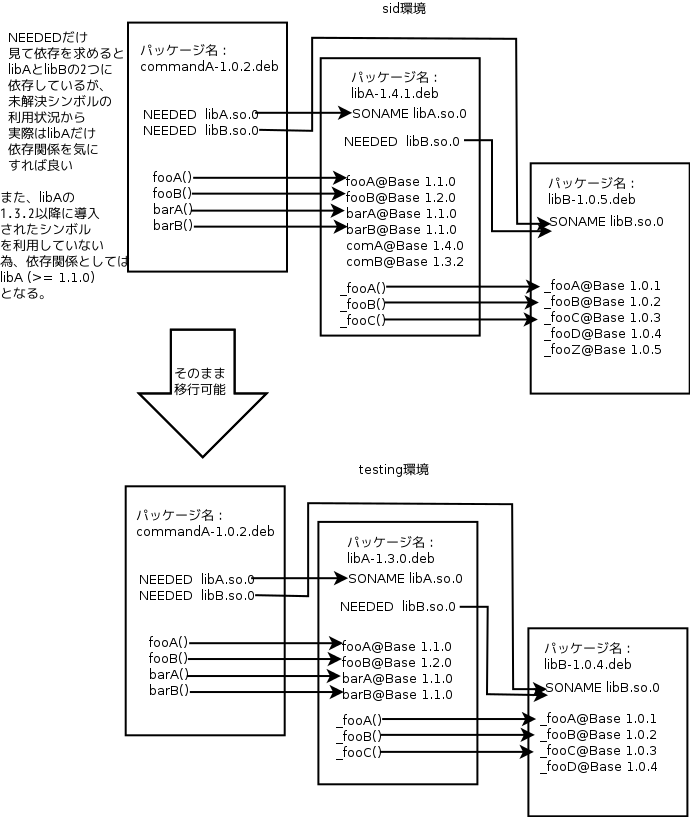
\includegraphics[width=12cm]{image201208/symbols-advantage.png}
\caption{\label{fig:symbol-deps}symbolファイルを利用した依存関係算出}
\end{center}
\end{figure}

という事を検討します。もし、こちらが出来ると、例えばsidからtesting
へバイナリパッケージを移動させるときに、依存関係にある数多くのライブラリ全部も同時に
sidからtestingへ完全に移動できるようになるまで、バイナリ本体をtestingの
ものとして移動出来ないという問題を極力避ける事ができます。\cite{hertzog}
(図\ref{fig:symbol-deps}参照)
    
\subsection{substvarsファイル}

 \$\{shlibs:Depends\}、\$\{shlibs:Recommends\}マクロなどのcontrolファイルに
含まれる情報を置き換える際にdebhelper共通で使われる中間ファイルとなります。
各debhelperコマンドがsubstvarsファイルに置き換えるべき内容を追記を繰り返すことにより、substvarsファイルは更新され、最後にdh\_gencontrolがマクロ部分をsubstvarsを参照しながら、適宜置き換えた制御ファイルとしてのcontrolファイルを生成します。

\subsection{内部で主に利用されているdpkgパッケージに含まれるコマンド}

 今回のdebhelperコマンドは内部でdpkgパッケージに含まれるいくつかのコマンド
を利用して処理を行っています。

\subsubsection{dpkg-gensymbols}

 dh\_makeshlibs内部にて、ライブラリメンテナがソースに含めているsymbolファイルを
元にし、実際に構築したライブラリから得られるシンボルの差分を含めたsymbolファイル
を生成するのに使われます。この生成されたsymbolファイルはライブラリ
パッケージのcontrolファイル群として含められます。

 dh\_makeshlibsの行うデフォルトの呼び出しでは、dpkg-gensymbolsは
ソースに含めているsymbolファイルからシンボルが廃止されたものがあることを
発見すると、DEBIAN/symbolファイルを一旦生成するものの、
エラーステータスを返却して終了してしまいます。この時、標準出力に違いを
diff形式で示します。もし、このような事が発生した場合は、メンテナはこのdiffを見ながら、
symbolファイルのメンテナンスを行う事になります。また、
生成されたsymbolファイルをメンテナは保管する事により、
次回のライブラリのバージョンアップに備える事になります。

\subsubsection{dpkg-shlibdeps}

 dh\_shlibdepsはほとんどdpkg-shlibdepsのラッパーコマンドとも
言えるぐらい、共有ライブラリの依存関係算出にあたって、
dpkg-shlibdepsをそのまま利用しています。

 dpkg-shlibdepsの動作は以下のとおりです。
\begin{description}
\item [Step 1.] コマンドラインから与えられたバイナリファイルが必要とする共有ライブラリへの
動的リンクに必要な情報を
\begin{commandline}
objdump -w -f -p -T -R バイナリファイル
\end{commandline}
コマンドを使って探ります。
\item [Step 2.] 得られた情報のうち、NEEDEDに記載されているSONAMEと同じファイル名を持つ
ライブラリファイルを\texttt{/lib},\texttt{/usr/lib}以下から探し当てます。
\item [Step 3.] 発見したライブラリファイルのフルパスを元にdpkg -Sを利用してライブラリの
パッケージ名を割り出します。
\item [Step 4.] ``\texttt{dpkg-query --control-path} ライブラリパッケージ名''を使って
\texttt{/var/lib/dpkg/info/}以下にあるライブラリパッケージの提供するshlibsファイル/
symbolファイルを取得します。
\item [Step 5.] Step 1.で得たバイナリファイルの動的リンクに必要なシンボル名と、
Step 4.で得たshlibsファイル/symbolファイルを検証することによりバイナリファイルにとって
最適な依存関係を算出します。
\item [Step 6.] substvarsファイルに算出した依存情報を記載します。
\end{description}

 参考: Step 5.の動作をどのように行っているかを観察するには、
\begin{commandline}
$ dpkg-shlibdeps -v -v -v -O バイナリファイル
\end{commandline}
%$
をバイナリファイルに対応するソースパッケージ展開後のディレクトリで、
実行するとよく判ります。

\subsubsection{おわりに}

 共有ライブラリの依存関係の対応すら2コマンドで担当出来るdebhelperコマンドと、
その心臓部を担うdpkgパッケージに含まれるコマンド群はよくできていると思いました。

\begin{thebibliography}{98}
\bibitem{levine} John R.Levine, 榊原 一矢/ポジティブエッジ 訳, ``Linkers \&
	 Loaders'', ISBN10 4274064379
\bibitem{sakai} 坂井 弘亮,  ``リンカ・ローダ実践開発テクニック'', ISBN10 4789838072
\bibitem{satorutakabayashi} 高林 哲ら, ``Binary Hacks'', ISBN10 4873112885
\bibitem{junichiuekawalibrary} Junichi Uekawa, ``Debian Library Packaging guide'',\url{http://www.netfort.gr.jp/~dancer/column/libpkg-guide/libpkg-guide.html}
\bibitem{man5deb} man 5 deb もしくはwikipediaのdeb(ファイルフォーマット),\url{http://ja.wikipedia.org/wiki/Deb_(%E3%83%95%E3%82%A1%E3%82%A4%E3%83%AB%E3%83%95%E3%82%A9%E3%83%BC%E3%83%9E%E3%83%83%E3%83%88)}

\bibitem{hertzog} 
Hertzog, ``Improved DpkgShlibdeps'', \url{http://wiki.debian.org/Projects/ImprovedDpkgShlibdeps}

\end{thebibliography}

%-------------------------------------------------------------------------------
\dancersection{月刊 Debian Policy 第5回 「ソースパッケージ」}{甲斐 正三}
%-------------------------------------------------------------------------------
\index{debian policy}
\index{source package}

\subsection {Debian ポリシーとは}
\begin{enumerate}
\item Debian ディストリビューションに要求されるいくつかの必要条件。
\item Debian アーカイブの構成と内容、オペレーティングシステムとしての Debian の設計に関するいくつかの事項
\item それぞれのパッケージがディストリビューションに受け入れられるために満たさなければならない技術的な必要条件。
\end{enumerate}

\subsection{ソースパッケージとは}
\begin{enumerate}
\item Debian バイナリパッケージの元になるパッケージである。

  (例)  シェルスクリプトの bash は bash というソースパッケージからビルドされる。
\item 一つのソースパッケージから複数のソースパッケージがビルドされることがある。

  (例)  bash ソースパッケージは bash バイナリパッケージ、bash-builtins、及び bash-doc パッケージもビルドされる。
\end{enumerate}

\subsection{ソースパッケージにおけるデビアンポリシーとは}
上記1と2から、

「 Debian GNU/Linux のソースパッケージの内部構成や、Debian GNU/Linux として必要なソースパッケージの設計指針についてまとめられたものである」

といえるのではないでしょうか。

\subsection{ソースパッケージに対するデビアンポリシーの実際}
それでは、「Debianポリシーマニュアル Chapter4 - ソースパッケージ」を見ながら、各項目を外観していくことにします。
以下の項目番号はマニュアルのそれに対応させています。なお、バージョン 3.9.1.0以降の更新された版については言及しません。


\begin{itemize}
\item 4.01 基準への準拠
  \begin{enumerate}
  \item 最新のパッケージング基準のバージョンを指定する。
  \item Standards-Version コントロールフィールドで指定。

    (ソースパッケージに含まれる'.dsc'ファイル中)
  \item 最新版を次のURLでチェックすること。

    \url{http://www.debian.org/doc/debian-policy/ch-scope.html#s1.2}
  \item 2012年7月21日現在の最新バージョン:

    'version 3.9.3.1, 2012-03-04'
  \end{enumerate}

\item 4.02 パッケージ同士の依存関係
  \begin{enumerate}
  \item ビルド時に必要なバイナリパッケージを明記すること。

    (ソースパッケージに含まれる'.dsc'ファイル中)
  \item ビルド時にインストールされていてはいけないパッケージも明記のこと。
  \item ただしbuild-essential パッケージは記載する必要は無い。
  \item 以下のパッケージのみで構成された環境でビルドできなければならない。
    \begin{description}
    \item essentialパッケージ、
    \item build-essentialパッケージ、
    \item 依存関係を満たすパッケージ。
    \end{description}
  \end{enumerate}

  \begin{itembox}[l]{'build-essentialパッケージ'とは何か見てみよう。}
    \url{http://packages.debian.org/ja/sid/amd64/build-essential/download}
    \begin{commandline}
# apt-get install build-essential && view /usr/share/doc/build-essential/essential-packages-list
  base-files base-passwd bash coreutils dash debianutils diffutils
  dpkg e2fsprogs findutils grep gzip hostname ncurses-base
  ncurses-bin perl-base sed login sysvinit-utils sysvinit
  tar bsdutils mount util-linux
    \end{commandline}
  \end{itembox}

\item 4.03 アップストリームのソースへの変更
  \begin{enumerate}
  \item パッケージをDebianまたはLinux向けにする際、ソースコード変更が生じた場合は、それがDebian固有の理由でないならアップストリームの作者へ変更依頼すべきである。
  \item 'Makefile'を修正したい場合は'Makefile.in'ファイルを修正する。'Makefile'を修正しても'configure'実行で消えてしまうので再現できない。
  \end{enumerate}

  \begin{itembox}[l]{ビルド手順の一例}
    \begin{commandline}
$ autoconf     // 'configure'スクリプトを生成。
$ ./configure  -> Makefile.inを読み込んでMakefileを生成。
$ make         // Malefileを読み込んでmakeする。
    \end{commandline}
    %$ for emacs font-lock
    * 各unix系OSの違いを自動的に吸収する手段
  \end{itembox}

\item 4.04 Debian changelog: debian/changelog
  \begin{enumerate}
  \item changelog への記載事項を規定
    \begin{itemize}
    \item 当該パッケージに対する修正や更新
    \item 上流の版に加えたDebian向けの修正や更新
    \item chanegelogへの記載フォーマットは厳密に決まっている。
    \end{itemize}
  \end{enumerate}

  \begin{itembox}[l]{実際にビルドしてみよう。}
    参照先(下記)の通りにやってみる。

    参照先:\url{http://www.debian.org/doc/manuals/maint-guide/build.ja.html}
  \end{itembox}

\item 4.05 著作権表記: debian/copyright
  \begin{enumerate}
  \item 各パッケージには著作権と配布条件のライセンス文書を元のままの形式で'/usr/share/doc/package/copyright'に収録すること。
  \end{enumerate}

\item 4.06 makefile でのエラーを捕捉する
  \begin{enumerate}
  \item makeする場合は上流で作られたmakefileにせよdebian/rulesにせよ、shを
    使うがshのエラー処理は不完全なため、debian/rulesはエラーを確実に捕捉
    できるようスクリプトを記述すること。

    (例) 2つ以上のコマンドをつなぐときは';'ではなく'\&\&'で。
  \end{enumerate}

\item 4.07 タイムスタンプ
  \begin{enumerate}
  \item 上流のソースファイルのタイムスタンプは可能な限り変更しないこと。
  \end{enumerate}

\item 4.08 ソースパッケージに含まれるものに対する制限
  \begin{enumerate}
  \item ソースパッケージに次のものは含まないこと。
    \begin{itemize}
    \item ハードリンク
    \item デバイスファイル
    \item ソケットファイル
    \item setuidやsetgidされたファイル
    \end{itemize}
  \end{enumerate}

\item 4.09 debian/rules - メイン構築スクリプト
  \begin{enumerate}
  \item debian/rulesとはソースパッケージからバイナリパッケージを構築する
    スクリプトである。
  \item  このファイルの先頭は'\#! /usr/bin/make -f'と記述すること。
  \item  スクリプトは非対話形式であること。
  \item  非対話的である必要最小限のターゲットは以下の5つ。

    (dpkg-buildpackageで呼び出されるターゲット)
    \begin{itemize}
    \item clean: ソースツリーのクリーン
    \item binary: ソースパッケージのビルド
    \item binary-arch: アーキテクチャ依存のバイナリパッケージをビルド
    \item binary-indep: オートビルダ\footnote{種々の移植版をサポート}システム使用時は不要。
    \item build: ビルド(コンパイル)を行いバイナリパッケージを構築する。
    \end{itemize}
    (詳細は割愛)
  \end{enumerate}

\item 4.10 変数置換 debian/substvars
  \begin{enumerate}
  \item  dpkg-gencontrolがDEBIAN/controlファイルを生成するが、このファイルに
    書き込む前に変数置換を行う。
  \item  事前に変数置換定義をdebian/subtvarsファイルに記述しておく。
  \item  変数置換は \${変数名} の書式を持つ。
  \item  変数置換の詳細の参照先: deb-substvars(5)
  \end{enumerate}

\item 4.11 上流のソースの場所の設定 (オプション) - debian/watch
  \begin{enumerate}
  \item 目的は新しく提供されたパッケージのアップデートをhttpまたはftpで
    走査できるようにすることである。
  \item このファイルはuscanユーティリティで使う。
  \item パッケージ品質管理とディストリビューション全体の保守のために
    使われている。
  \item 使用例
    \url{http://dehs.alioth.debian.org/} および他のDebian QA ツール。
  \end{enumerate}

\item 4.12 debian/files
  \begin{enumerate}
  \item このファイルはパッケージビルド中に生成されたファイルを記録する
    ための一時ファイルである。
  \item dpkg-genchanges は、``.changes'' ファイルを生成するときにこれを用いる。
  \item このファイルをアップロードされるソースパッケージに含めてはいけない。
  \item これらのファイルは、clean ターゲットによって削除すること。
  \item binary ターゲットを開始する際には、これらのファイルを削除するか空に
    すること。
  \item dpkg-gencontrol を実行した際に、debian/files に追加されるエントリも
    clean ターゲットで削除すること。
  \item ソースパッケージと、 dpkg-gencontrol によってコントロールファイルが
    生成されたバイナリパッケージ以外のファイルはパッケージのトップ階層
    ディレクトリの親ディレクトリに置くこと。
  \item debian/files のリストにファイルを追加する場合はdpkg-distaddfile を
    呼ぶこと。
  \end{enumerate}

\item 4.13 コードの便宜的写し
  \begin{enumerate}
  \item Debian パッケージに、他のパッケージのコードの写しを直接組み込むことは
    しないこと。
  \item もし、組み込みたいコードが Debian アーカイブライブラリであるなら、
    バイナリパッケージからライブラリ参照を行なうとよい。
  \item もし組み込みたいコードが Debian に収録されていない場合は、可能ならば
    そのコードを、前提の依存関係を付けて別にパッケージングすべきである。
  \end{enumerate}

\item 4.14 ソースパッケージの処理: debian/README.source
  \begin{enumerate}
  \item dpkg-source: Debian ソースアーカイブの作成、展開を行う。
  \item dpkg-source -x filename.dsc [output-directory]:

    ソースパッケージをDebian ソースコントロールファイル (.dsc) 名として
    展開先ディレクトリoutput-directoryに展開する。
  \item dpkg-buildpackage :  バイナリパッケージおよびソースパッケージをビルドする。
  \item dpkg-source -x をソースパッケージに対して実行しても、直ぐ編集可能で、
    変更を加えた後修正されたパッケージを追加作業なしに dpkg-buildpackage で
    作成できるようなパッケージのソースが得られない場合には、
    debian/README.source 解説ファイルの追加をする。
  \item debian/README.source 解説ファイルには、以下のすべての手順が説明されて
    いなければならない。
    \begin{itemize}
    \item 全部のパッチが当たったソースを作成する方法。(debian/rules の
      patch ターゲットで行なえるようにする。)
    \item ソースを変更し、その変更をセーブしてパッケージ作成の際に適用できる
      ようにする方法。
    \item パッケージをビルドする際に、現在当てられているソース修正をすべて元に
      戻す方法。
    \item 新しい上流の版が出た場合、Debianソースパッケージをアップグレードする
      手順。(可能なら)
    \item この説明は具体的なコマンド名やパッケージ名にまで言及すべきである。
    \item この説明はDebianパッケージシステムや管理ツールを熟知していなくても
      理解できるように記述すべきである。
    \end{itemize}
  \end{enumerate}
\end{itemize}

以上

\subsection{参考文献}
\begin{enumerate}
\item 「Debian ポリシーマニュアル バージョン 3.9.1.0, 2011-07-05」

  \url{http://www.debian.or.jp/community/devel/debian-policy-ja/policy.ja.html/ch-source.html}
\item 2006年4月15日 「第15回東京エリアDebian勉強会事前配布資料」\\
\url{http://tokyodebian.alioth.debian.org/pdf/debianmeetingresume200604.pdf}
\item 「Debian 新メンテナーガイド 第6章 パッケージのビルド」

\url{http://www.debian.org/doc/manuals/maint-guide/build.ja.html}

\end{enumerate}

%-------------------------------------------------------------------------------
\dancersection{月刊 Debian Policy 第6回 「文書」}{岡野 孝悌}
%-------------------------------------------------------------------------------
\index{debian policy}

Debian ユーザーでもないのに今回の担当となりました おかの です。

今回読むのは第12章の「文書」についてです。
多くのソフトウェアパッケージにはマニュアルなどの文書が附属していますし、文書のみからなるパッケージもあります (debian-policy 自体がまさにそうです)。
また、マニュアル類のほか、設定ファイルのサンプルや、変更履歴、著作権情報といったものもあります。

\subsection{マニュアル (man ページ)}
ベル研で Unix が誕生したころ、文書処理システムという口実で予算を取っていたりして、
Unix 関係の文書といえば roff でした\footnote{History of UNIX Manpages http://manpages.bsd.lv/history.html が参考になります。}。
本章でも man ページの説明に多くを割いています。
\index{roff}

\subsubsection{インストール場所}
roff ファイルを gzip -9 で圧縮して、
{\tt /usr/share/man} 以下の適切な場所にインストールします。
英語マニュアルは {\tt /usr/share/man} 直下、
それ以外は {\tt /usr/share/man/}{\it locale} 以下の、
セクション別のディレクトリ ({\tt man1}, {\tt man2}, ..., {\tt man9}) に置きます。
詳細は FHS 参照といいつつ、FHS とは以下のような差異があります。

\begin{itemize}
\item 英語マニュアルは {\tt /usr/share/man/en} 以下ではなく {\tt /usr/share/man} 直下に置く。
(FHS でこれが許されるのは、英語マニュアルしかない場合)
\item セクション 9 が存在する
(FHS では 1 から 8 までのみ)
\end{itemize}

man ページの整形には時間がかかるので、
整形済みのマニュアルをあらかじめインストールしておけば\footnote{FreeBSD のベースシステムなどでは整形済みのマニュアルが標準で配布されています。}、
いきなりページャーで表示することができて快適になりますが、
パッケージが整形済みマニュアルをインストールしてはいけません。

\subsubsection{パッケージへの同梱}
man ページ以外の文書は、{\it foo}-doc のようにソフトウェア本体と別パッケージに分離することがありますが、
man ページはソフトウェア本体と同じパッケージに含めるのが原則です。

プログラムのマニュアルが存在しない場合、それはバグとして扱われます。
上流にマニュアルを追加してもらうか、Debian パッケージで独自にマニュアルを追加する必要があります\footnote{現在はバグのあるパッケージはそもそもアップロードできないので、man がないパッケージはありえないことになります}。
といっても、「info 見れ」「この URL 見れ」だけのマニュアル\footnote{そのようなマニュアルの実例としては、(いずれも上流由来ですが) GNU cpio や netpbm があります。}でも可です。
これは、とにかく man を見れば情報に辿り着けることを保証する、という考えにもとづいています。

\subsubsection{複数名をもつマニュアル}

grep, fgrep, egrep のように、同じマニュアルが複数の名前で参照されることがあります。

Linux Man Page Howto\footnote{\url{ http://www.schweikhardt.net/man_page_howto.html} (JF に古い日本語訳あり)}
では、(シンボリックリンクを持たないシステムに配慮し) roff の .so マクロを使う方法がもっとも望ましいとされていますが、
Debian では必ずシンボリックリンクがあるためか、原則として .so マクロを使わずにシンボリックリンクを使うよう求めています。
ただし、上流で .so マクロを使っている場合は、無理にシンボリックリンクに直す必要はありません。

たとえば grep パッケージ (GNU grep) では、egrep.1.gz, fgrep.1.gz はいずれも grep.1.gz へのシンボリックリンクとなっています。
いっぽう、manpages-ja パッケージにはこれらの (古い) 日本語訳がありますが、こちらでは egrep.1 や fgrep.1 は .so マクロを使って grep.1 を参照しています。

なお、これとは逆に、複数の異なるマニュアルが同じ名前で参照されることがあります。たとえば vim と nvi は、通常どちらも vi という名前で参照されます。
本章では言及されていませんが、これは Appendix F で説明されている update-alternatives で扱うことができます。
また、editor(1) と pager(1) について11章で言及されています。

\subsubsection{翻訳マニュアル}

マニュアル以外の文書にも翻訳はありますが、debian-policy ではマニュアルについてのみ翻訳に触れています。
マニュアルはガンガン更新されるので、せっかく翻訳してもすぐ古くなってしまいます。
利用者が古い翻訳マニュアルを鵜呑みにしないように、翻訳が古い可能性について言及したりするよう求めています。

apt など、Debian 独自ツールのマニュアル翻訳では、po4a を使って翻訳し (訳が古くなった場合、その部分は原文が表示されるようになる)、
かつ注意書きをすることで、この指針が守られているようです。
一方、manpages-ja をはじめ、上流で翻訳されたマニュアルでは、守られていないように見えます。

エンコーディングは UTF-8 のほか、一部のレガシーエンコーディング (日本語の場合は EUC-JP) も使えます\footnote{man のエンコーディングに関する議論は Bug\#440420 参照}。

\subsection{info 文書}

info 文書について述べています。info 文書は必須ではありません。

\begin{itemize}
\item info 文書は {\tt /usr/share/info} 以下へインストールする
\item gzip -9 で圧縮する
\item install-info 用のセクションとディレクトリエントリ情報を含める
\end{itemize}

\subsection{追加文書}

man, info 以外の形式の文書がパッケージに含まれている場合の扱いを述べています。

\begin{itemize}
\item info は {\tt /usr/share/doc/}{\it package} 以下へインストールする
\item 大容量で必要性の低い文書は別パッケージにするべき
\item ソフトウェアの動作が {\tt /usr/share/doc/}{\it package} 以下のファイルに依存してはいけない
\item {\tt /usr/share/doc/}{\it package} 自体を他へのシンボリックリンクとできる条件 (著作権関連情報の節にも記載がありますが、適切な copyright ファイルを機械的に抽出できる必要があります)
\item {\tt /usr/doc} から {\tt /usr/share/doc} への移行に関する説明\footnote{脚注にも説明がありますが、
FSSTND 1.2 までは、{\tt man} や {\tt doc} 等は{\tt /usr/} 直下に置くこととなっていました。
FHS 2.0 (1997 年) で、BSD の流儀を取り入れ、{\tt /usr/share/} 以下に置くよう改められています。
Debian では potato で移行しています。当時の議論は 1999 年からの debian-ctte メーリングリストのログで見ることができます。}
\end{itemize}

\subsection{好ましい文書形式}

DocBook などをもとに同じ文書を複数形式で提供するケースがありますが、
そのような場合は可能な限り HTML をインストールします。
HTML 以外の形式をどうするかはメンテナーの裁量にまかされています。

\subsection{著作権関連情報}

パッケージに含まれるものの著作権、ライセンスに関する文書 ({\tt copyright} ファイル) の扱いについて述べています。このファイルは必須です。

Debian パッケージでは {\tt debian/copyright} に含めておき、
{\tt /usr/share/doc/}{\it package}{\tt /copyright} にインストールします。

このファイルには、パッケージの著作権、ライセンス情報を、元のままで含める必要があります
(ただし、GPL などのよく使われるライセンスは {\tt /usr/share/common-licenses} にあらかじめ置かれているものを参照する形にします)。
内容の改変はもとより、文書形式の変換もしてはいけません。
また、このファイルを圧縮したりシンボリックリンクにしたりしてはいけません。

{\tt copyright} ファイルには、著作権、ライセンス情報のほか、以下の情報を含める必要があります。

\begin{itemize}
\item 上流のソースの入手元
\item パッケージの原作者名
\end{itemize}

また、以下の情報を含めるべきです。

\begin{itemize}
\item Debian パッケージ作成に関与した Debian メンテナ名 (3.9.3.0 で削除されました; 後述)
\item (contrib, non-free の場合) 当該パッケージが Debian の一部ではないことと、その簡潔な理由
\end{itemize}

\subsection{設定例など}

設定ファイルやソースファイルなどの例を提供する場合の扱いを述べています。

\begin{itemize}
\item {\tt /usr/share/doc/}{\it package}{\tt /examples} 以下にインストールする。
\item ただし、アーキテクチャー依存のファイルは
{\tt /usr/lib/}{\it package}{\tt /examples} 以下にインストールし、
シンボリックリンクを張る。
\item 前述のとおり、動作が {\tt /usr/share/doc} 以下のファイルに依存してはいけないので、
ここに置かれたファイルをプログラムから参照してはいけない。
\item {\it foo}-examples のような、例そのものを提供するパッケージは、
パッケージそのものを {\tt /usr/share/doc/}{\it package} にインストールしてもよい。
\end{itemize}

\subsection{Changelog ファイル}

変更履歴の扱いについて述べています。

Debian 由来でないパッケージは、上流の変更履歴と Debian パッケージの変更履歴を区別することを求めています。

\begin{itemize}
\item Debian ソースツリー内の
{\tt debian/changelog} の圧縮されたコピーを
{\tt /usr/share/doc/}{\it package}/{\tt changelog.Debian.gz} としてアクセスできるようにしなければならない。
\item 上流の changelog がある場合は、プレインテキスト形式で、
{\tt /usr/share/doc/}{\it package}{\tt /changelog.gz} としてアクセスできるようにすべき。
\item changelog ファイルが HTML 形式の場合は、
{\tt /usr/share/doc/}{\it package}{\tt /changelog.html.gz} で参照できるようにすべき。
\item 上流のファイル形式の違いによって、別のファイル名を参照しないといけないなどというのはウンコなので、
Lynx を使って HTML をプレインテキストに変換したものを {\tt /changelog.gz} で提供すべき。
\item gzip -9 で圧縮すべき
\end{itemize}

\subsection{最近の変更点}
日本語訳版がある Version 3.9.1.0 から Version 3.9.4.0 までに加えられた変更点を押さえておきましょう。

\subsubsection{Version 3.9.2.0}
\begin{itemize}
\item 「Debian GNU/Linux ディストリビューション」が「Debian ディストリビューション」と改められました。(Bug\#594656)
\item debmake で生成される man のサンプルについて言及されていましたが、lenny 以降では debmake は削除されているため、この記述が削除されました。
\end{itemize}

\subsubsection{Version 3.9.3.0}
\begin{itemize}
\item {\tt copyright} ファイルに Debian パッケージのメンテナーを記述することとされていましたが、{\tt changelog} ファイルに書かれているものなので、{\tt copyright} ファイルへの記述がなくなりました。(Bug\#593533)
\end{itemize}

\vspace{1ex}
\hrule
\subsubsubsection{Version 3.9.2.0 policy.sgml:9771}\par
\parbox{0.48\linewidth}{
	  In addition, the copyright file must say where the upstream
	  sources (if any) were obtained.  It should name the original
	  authors of the package and the Debian maintainer(s) who were
	  involved with its creation.
}\hfil 
\parbox{0.48\linewidth}{
	  また、著作権情報ファイル中には元となった上流のソースをどこから手に入れたかを記載しなければなりません。
	  またパッケージの原作者の名前とパッケージ作成に関与した
	  Debian メンテナの名前を載せるべきです。
}
\hrule

\subsubsubsection{Version 3.9.3.0 policy.sgml:9863}\par
\parbox{0.48\linewidth}{
	  In addition, the copyright file must say where the upstream
	  sources (if any) were obtained, and should name the original
	  authors.
}\hfil 
\parbox{0.48\linewidth}{
	  また、著作権情報ファイル中には元となった上流のソースをどこから手に入れたかを記載しなければなりませんし、
	  パッケージの原作者の名前を載せるべきです。
}
\hrule
\vspace{1ex}

\begin{itemize}
\item 「機械的に抽出」できるようにするもの ({\tt copyright} ファイル) が何を指しているかが、明確に記述されるようになりました。(Bug\#617516)
\end{itemize}

\vspace{1ex}
\hrule
\subsubsubsection{Version 3.9.2.0 policy.sgml:9704}\par
\parbox{0.48\linewidth}{
	  {\tt /usr/share/doc/}{\it package} may be a symbolic
	  link to another directory in {\tt /usr/share/doc} only if
	  the two packages both come from the same source and the
	  first package Depends on the second.  These rules are
	  important because copyrights must be extractable by
	  mechanical means.
}\hfil 
\parbox{0.48\linewidth}{
	  {\tt/usr/share/doc/}{\it package}
	  は、{\tt /usr/share/doc}
	  以下の他のディレクトリ中のシンボリックリンクの相手先と同じソースファイルから作成されたものであること、および相手先に対して
	  ``Depends'' で依存していることが宣言されていること、の二つの条件を満たすときのみ、シンボリックリンクとすることができます。
	  この規則は、著作権関連ファイルが機械的に抽出できるようにするために大切になるものです。
}
\hrule

\clearpage

\subsubsubsection{Version 3.9.3.0 policy.sgml:9796}\par
\parbox{0.48\linewidth}{
	  {\tt /usr/share/doc/}{\it package} may be a symbolic
	  link to another directory in {\tt /usr/share/doc} only if
	  the two packages both come from the same source and the
	  first package Depends on the second.  These rules are important
	  because {\tt copyright} files must be extractable by
	  mechanical means.
}\hfil 
\parbox{0.48\linewidth}{
	  {\tt/usr/share/doc/}{\it package}
	  は、{\tt /usr/share/doc}
	  以下の他のディレクトリ中のシンボリックリンクの相手先と同じソースファイルから作成されたものであること、および相手先に対して
	  ``Depends'' で依存していることが宣言されていること、の二つの条件を満たすときのみ、シンボリックリンクとすることができます。
	  この規則は、{\tt copyright} ファイルが機械的に抽出できるようにするために大切になるものです。
}
\hrule
\vspace{1ex}

\begin{itemize}
\item 機械可読な著作権情報ファイルに関する記述が追加されました。ライセンス衝突などの問題を自動的にチェックしたりできることが期待できますが、今のところはオプション扱いです。
\end{itemize}

\vspace{1ex}
\hrule
\subsubsubsection{Version 3.9.3.0 policy.sgml:9928}\par
\parbox{0.48\linewidth}{
	  {\bf Machine-readable copyright information}

	    A specification for a standard, machine-readable format
	    for {\tt debian/copyright} files is maintained as part
	    of the {\it debian-policy} package.  This
	    document may be found in the {\tt copyright-format}
	    files in the {\it debian-policy} package.  It is
	    also available from the Debian web mirrors at
		     \url{http://www.debian.org/doc/packaging-manuals/copyright-format/1.0/}.

	    Use of this format is optional.
}\hfil 
\parbox{0.48\linewidth}{
	  {\bf 機械可読な著作権情報}

	    標準のための仕様として、機械可読な形式の
	    {\tt debian/copyright} ファイルが、
	    この {\it debian-policy} パッケージの一部として保守されています。
	    この文書は {\it debian-policy} パッケージに
	    {\tt copyright-format} ファイルとして含まれています。
	    また、Debian web ミラーの
		     \url{http://www.debian.org/doc/packaging-manuals/copyright-format/1.0/} にもあります。

	    この形式を使うかどうかは任意です。
}
\hrule
\vspace{1ex}

\subsubsection{Version 3.9.3.1}

(変更なし)

\subsubsection{Version 3.9.4.0}
\begin{itemize}
\item {\tt copyright} ファイルのエンコーディングに関する一文が追加されました。(Bug\#661933)
\end{itemize}

\vspace{1ex}
\hrule
\subsubsubsection{Version 3.9.1.0 policy.sgml:10673}\par
\parbox{0.48\linewidth}{
	  All copyright files must be encoded in UTF-8.
}\hfil 
\parbox{0.48\linewidth}{
	  copyright ファイルはすべて UTF-8 でエンコードしなければなりません。
}
\hrule
\vspace{1ex}

\subsection{最後に}
次回の月刊 Debian Policy は。。。

%-------------------------------------------------------------------------------
\dancersection{ソフト開発以外の簡単Debian contribution}{野島 貴英}
%-------------------------------------------------------------------------------
\index{かんたんなこんとりびゅーしょん@簡単なコントリビューション}

\subsection{はじめに}

 以前debconf11に参加した時、debconfの最後に行われるライトニング
トークで、「ソフト開発以外にDebianへ貢献するにはこんなのが
あるよ!」という発表がありました。この発表を聞いて以降、このあたりを
一度まとめてみたいなーと思っていました。

 ここでは、Debianをインストールしてちょっと慣れたぐらいの人がちょこちょこっと
Debianへ貢献する手段についてまとめてみます。きっと漏れもあると思うので、東京エリアDebian勉強会にてBOF形式で補完してみます。

\subsection{ソフト開発以外の簡単contribution作業一覧(ドラフト版!)}

\begin{itemize}
\item DDTSSの日本語訳をレビューしてみる、日本語に訳してみる。\\
(詳しくは「第53回東京エリアDebian勉強会資料」\url{http://tokyodebian.alioth.debian.org/pdf/debianmeetingresume200906.pdf}を参照ください。非常に良い解説とチュートリアルとなっています。)
\item BTSへBUG報告/何かの改善提案をしてみる。\\
(詳しくは「第43回 関西Debian勉強会資料」\url{http://wiki.debian.org/KansaiDebianMeeting/20110123}を参照ください。非常に良い解説とチュートリアルとなっています。)
\item \url{http://debtags.debian.net/edit/}でdebtagsをひたすら打ち込む。\\
(詳しくは「第63回東京エリアDebian勉強会資料」\url{http://tokyodebian.alioth.debian.org/pdf/debianmeetingresume201004.pdf}を参照ください。非常に良い解説とチュートリアルとなっています。)
\item \url{http://screenshots.debian.net/}へスクリーンショットを投稿しまくってみる。
\item \url{http://www.debianart.org/cchost/}へオリジナルの絵を送ってみる。
\item \url{debian-doc@debian.or.jp}にて投稿された翻訳のレビューをしてみる、未だ日本語に訳されていない文章を翻訳して投稿してみる。
\item \url{debian-users@debian.or.jp}にて投稿された質問に回答をしてみる。
\end{itemize}

\subsection{screenshots.debian.net}
\index{screenshots.debian.net}

 パッケージの動作のスクリーンショットを集めているサイトです。synapticパッケージマネージャ(aptitude install synapticで導入できます)にはプログラムの紹介の他に、プログラムが動作しているときのスクリーンショットを見る事ができます。このスクリーンショットのダウロード先がこのscreenshots.debian.netとなります。

 初めての方は以下のようにしてスクリーンショットを投稿できます。アカウント登録すら不要のお手軽サイトなので、面倒なユーザ登録も必要ありません。こちらに投稿され、無事審査をパスしたスクリーンショットは、世界中のDebianユーザが使っているsynapticパッケージマネージャで即閲覧できるようになります。

以下にスクリーンショットの投稿の仕方を記載します。

 \begin{description}
 \item [Step 1.] \url{http://screenshots.debian.net/packages/without_screenshots?search=&debtag=}をアクセスし、スクリーンショットが無いパッケージから適当なものを選びます。
 \item [Step 2.] 選んだパッケージを手元のDebianマシンへ導入します。
 \item [Step 3.] export LANG=Cを実行して、表示されるメッセージができるだけ英語になるようにしてプログラムを起動出来るようにします。
 \item [Step 4.] 導入したプログラムを起動します。
 \item [Step 5.] プログラムのスクリーンショットを撮ります。GNOME環境であれば、ALT+Print Screenでスクリーンショットを撮る事の出来るアプリケーションが起動します。
 \item [Step 6.] PNGファイルで撮ったスクリーンショットの画像を保存し、ImageMagickなどを使って画像サイズを最大でも800x600ぐらいにしてPNG形式で保存します。
 \item [Step 7.] \url{http://screenshots.debian.net/upload}をアクセスして、パッケージ名(Package name:)、パッケージのバージョン(Software version:)、どこの画面か等の説明(Screenshot description:)のフォームを半角英数字で埋め、ScrrenshotのChoose Fileを選んで、先ほど保存したスクリーンショット画像を選択します。
\item [Step 8.] 最後に[Upload screenshot]というボタンをクリックすると早速投稿が完了します。この時点では、サイト管理チームの審査が終ってないので、1日ぐらい待ちます。
\item [Step 9.] 無事審査がパスされると、\url{http://screenshots.debian.net/}の左上あたりの``Latest uploads...''という部分に、投稿したスクリーンショットが掲載されます。この時点で、synapticパッケージマネージャからもスクリーンショットが閲覧できるようになります。
\end{description}

やってみると判りますが、非常に簡単です。パッケージの魅力を伝えるのに、スクリーンショットの影響は少なくないと自分も考えています(特にゲームのパッケージ)。ぜひこの機会にスクリーンショットをあげまくってみてください。

 なお、注意事項として、撮影するスクリーンショットの元となるデータのライセンスには十分気をつけてください。これは大方のパッケージでは意識しなくても全く問題ないのですが、ゲーム等のパッケージのうちゲーム機/元々有料ソフトのエミュレータ環境等の、エミュレータのスクリーンショットでは、表示に使ったデータ次第では十分にライセンスが問題になり得ます。このあたりがちょっとでも心配な方は、ゲームのエミュレータ環境のスクリーンショットを投稿するのは、ライセンスに自信のある方以外は止めておいた方がよいでしょう。

\subsection{debianart.net}
\index{debianart.net}

 Debianに使われる様々なグラフィック/サウンドデータの投稿サイトとなります。直近では、wheezyの起動画面の背景画像、GNOME環境のデフォルトの背景画像などのコンテストが行われました。

 最近では、Debianプロジェクトにマスコットキャラクタが必要ということで、
マスコットキャラクタの図案の募集が行われていたようです。

 絵心のある方/写真撮影に興味のある方/サウンドアイコンに興味ある方で、我こそはという方はぜひ活用すると良いかもしれません。

 なお、Debianのプロジェクトである以上、投稿した絵/写真/音楽はいわゆるフリーなライセンスで扱われる事が出来るものに限ります。こちらはご注意ください。

\subsection{おわりに}

 Debianは多様性を重視するプロジェクトです。ソフト開発以外の貢献は大変重要で、協力者は日夜必要な状態です。やってみようという方は是非ご協力お願いします。


%-------------------------------------------------------------------------------
\dancersection{本気で ``使える'' 翻訳環境を構築してみた}{八津尾 雄介}
%-------------------------------------------------------------------------------
\index{ほんやく@翻訳}

\subsection{はじめに - 今日の主旨}
アプリケーションのローカライズに man ページ、wiki 等々、普段何気にお世話に
なっている翻訳ですが、OSS の世界では (当然ですが) 有志によって行われています。
しかし、日本の OSS コミュニティにおいて翻訳者の不足はどのプロジェクトでも共通
の課題らしいということをよく耳にします。翻訳は高い技術力を必要とせず、誰でも簡
単に参加できます。翻訳支援ツールを使い、翻訳のプロセスを簡略かつ明確にすること
で、さらに参加する為の敷居が下がるのではないでしょうか?ということで、翻訳ツー
ルを利用した翻訳環境の構築事例を紹介していきたいと思います。

今回は翻訳ネタ2本立てという事で、トランスレータとして各プロジェクトに参加中
の皆さん、またこれから翻訳に参加してみようかとお考えの皆さんと一緒に、
翻訳環境について議論していきたいと思いますので積極的な発言をお願いします。

\subsection{DPN の翻訳効率化}
Debian Project News (以下、DPN ) の翻訳に参加しはじめてから半年が過ぎま
した。DPN を翻訳していくなかで、いくつか気づいた事があります。

\begin{itemize}
    \item ほぼ同じ内容の文章を何度も訳している
    \item 担当者が過去記事を参照せず、同一の事象での訳語が統一できていない
    \item グロッサリが存在せず、担当者間で訳語が統一できていない
    \item 明確なスタイルガイドラインが存在せず、暗黙のルールで運営されている
    \item 過去に訳した膨大な量の訳文 (=資産) を活かしきれていない
\end{itemize}

このような無駄を無くし、翻訳を効率化するために{\tt 翻訳メモリ}が活用できるの
ではないかと考え、現在快適な翻訳環境作りに取り組んでいるころです。私が考える
翻訳環境の柱は次のようになります。

\begin{itemize}
    \item 訳語を意識せずに揃えること
    \item 誰が翻訳しても同一の品質を保てること
    \item 過去の翻訳結果を再利用できること
    \item 翻訳プロジェクトのメンバ内でこれらの結果を共有できること
\end{itemize}

\subsubsection{翻訳メモリとは?}
{\tt 翻訳メモリ}とは、``ソースの言語とターゲットの言語を 1 対 1 で保存した
データベースのようなもの'' /です。
{\tt 翻訳メモリツール}は、翻訳メモリから類似の文章を探し出しヒット率が高い
文章の訳文を提示したり自動挿入や置換をする事で翻訳の支援を行うツールです。

よく勘違いされるのですが、{\tt 翻訳メモリツール}は勝手に翻訳してくれる機械翻
訳のようなものではありません。{\tt 翻訳メモリ}は自分で育てる必要があり初期状
態では全く使いものになりません。また、{\tt 翻訳メモリツール}は訳文の正確性の
判断はできないので、翻訳メモリに誤訳が混入しそれが繰り返し利用されてしまう可能
性がある事を常に念頭に置いておきましょう。

{\tt 翻訳メモリ}には{\tt TMX (Translation Memory eXchange)}という
XML ベースの規格があり、広く利用されています。
\footnote{もともと LISA (Localization Industry Standards Associa
	tion) によって策定された規格。2011年、LISA は破産宣告によって解散し、
	LISA で策定された他の規格と共にパブリックドメインへと帰した。}
\index{TMX}

産業翻訳でデファクトスタンダードとなっている
{\tt SDL TRADOS \textregistered}\footnote{http://www.trados.com}
や、本セッションで紹介予定の {\tt OmegaT}
\footnote{http://www.omegat.org} もこの{\tt TMX}を採用しています。
{\tt 翻訳メモリ}の更に詳しい概要と {\tt OmegaT} の操作方法については、
2011 年 10 月の関西 Debian 勉強会資料に掲載されている拙著「翻訳で Debian
に貢献しよう」も参考にしてください。

\subsubsection{定型記事と翻訳メモリ}
翻訳メモリがその真価を発揮できるのが、ある程度定型化された記事を
翻訳する場合です。以下の文例を見て下さい。

\begin{itembox}[c]{DPN2012 issue 15 より}
    \begin{verbatim}
<toc-add-entry name="newcontributors">New Debian Contributors</toc-add-entry>
	<p>
    Seven applicants have been
    <a href="https://nm.debian.org/public/nmlist#done">accepted</a>
    as Debian Developers, nine applicants have been
    <a href="http://lists.debian.org/E1Sta5X-0005lb-Ap@franck.debian.org">accepted</a>
    as Debian Maintainers, and six people have
    <a href="http://udd.debian.org/cgi-bin/new-maintainers.cgi">started to
    maintain packages</a> since the previous issue of the Debian Project News.
    Please welcome (著者注:中略 ここで人名が列挙される) into our project!</p>
    \end{verbatim}
\end{itembox}
\begin{itembox}[c]{DPN2012 issue 17 より}
    \begin{verbatim}
<toc-add-entry name="newcontributors">New Debian Contributors</toc-add-entry>
	<p>
    Three applicants have been
    <a href="https://nm.debian.org/nmlist.php#newmaint">accepted</a>
	as Debian Developers,and two people have
    <a href="http://udd.debian.org/cgi-bin/new-maintainers.cgi">started to
    maintain packages</a> since the previous issue of the Debian Project News.
    Please welcome (著者注:中略 ここで人名が列挙される) into our project!</p>
    \end{verbatim}
\end{itembox}

これらの記事はほぼ同じ内容であり、毎月必ず掲載される記事です。にも関わらず、
Debian-www メーリングリストで配布される原文に添付されている、おそらく何かの
スクリプト処理によって生成されたと思われる試訳では全く訳されません。翻訳メモリ
で一度でも訳しておけば、以降は訳文候補として過去の訳が参照できるのでこのような
記事をシームレスに翻訳することができます。では、実際に {\tt OmegaT} でどの
程度効率化できるのか試してみましょう。なお、ここでは {\tt OmegaT} の詳しい
使い方は説明しませんが、起動時に表示されるお手軽スタートガイドに目を通すだけで
一通りの作業はこなせるようになるでしょう。

\begin{itembox}[l]{DPN2012 issue 15 の日本語訳}
    \includegraphics{image201210/omegat_demo1.eps}
\end{itembox}

\begin{itembox}[l]{DPN2012 issue 17 を訳しているところ}
    \includegraphics{image201210/omegat_demo2.eps}
\end{itembox}

このように、翻訳メモリを利用することで訳語の揺れを減らし訳文の品質を高めること
ができます。

\subsubsection{訳語の統一}

担当者が変わったり単に翻訳者が以前当てた訳語を忘れてしまい、訳語から統一感が失
われてしまうという問題はしばしば発生します。この問題に対処する為にはグロッサリ
のメンテが必要不可欠です。

訳語を決めたらグロッサリに登録しておきましょう。{\tt OmegaT} の場合は UTF-8 の
タブ区切り形式でグロッサリを作成しておくことができます。
\footnote{複合語に難があったりとあまり洗練されていない}
残念ながら、現在メンテされていませんが{\tt OmegaT} で利用できる Debian 翻訳用
のグロッサリも入手可能です。
\footnote{Debian JP Doc/WWW 対訳表:http://www.debian.or.jp/community/translate/}
私は現在個人でグロッサリの作成とメンテをしていますが、本来であればプロジェクト
単位で準備すべきものです。グロッサリを整備しておくことで、新規参入者が迷わずに
翻訳を始められるのではないでしょうか。

\subsubsection{マークアップと翻訳メモリ}
DPN は {\tt wml} という {\tt html} によく似た {\tt xml} の拡張フォーマットで
記述されたものがメーリングリストで配布され、それを各担当者が訳しています。
{\tt OmegaT} を利用する時に注意が必要な事は、{\tt wml} がサポートされていない
という事です。
{\tt OmegaT} でサポートされていないファイルフォーマットは翻訳対象ファイルから
見えません。他にも、古いドキュメント類に散見される {\tt sgml} などはサポート
されていないので、ちょっとしたトリックでこれを翻訳できるようにしましょう。
\index{OmegaT}

もっとも簡単な方法はテキスト形式にしてしまうことです。翻訳対象ファイルの拡張子
を *.txt にしても良いですし、*.txt のファイルフィルタに翻訳したいファイルを登
録する方法もあります。しかしこの方法を使うと、タグの中まで翻訳対象となってしま
い翻訳メモリの能力を最大限引きだす事ができません。テキスト形式にしてしまう前に、
近いフォーマットのフィルタを試してみると良いでしょう。
私は {\tt wml} に {\tt html} のフィルタを使用しています。いまのところ
問題なく使えています。
\footnote{OmegaT の Okapi プラグインで対応ファイルを増やす方法もある}

\subsubsection{翻訳ツール}
翻訳メモリを導入することで、私が必要としていることの大半は実現できましたが、
理想の環境とはほど遠いのが現状です。まだまだ試行錯誤の段階では
ありますが、私が現在 DPN の翻訳に使用しているツールを紹介します。

\begin{itemize}
\item DPNToolKit.py -
	自作の python スクリプトです。{\tt wml} ファイルを分解し {\tt OmegaT}
	 のプロジェクトフォルダに配置したり、{\tt OmegaT} が生成した訳文から
	査読メール用の文章を生成したりします。
\item Debian JP Doc/WWW 対訳表
    一応導入し、個人的にメンテしています。{\tt OmegaT} から参照可能です。
\item 英辞郎 -
    言わずと知れたオンライン辞書です。第3版とオンライン版を適宜使い分けていま
    す。{\tt OmegaT} から参照可能です。
\item Google翻訳 -
    私が知っている機械翻訳の中で、最も精度の高い翻訳結果を出すのが Google翻訳
    です。機械翻訳はあくまで参考に使用する程度にしましょう。
\item vim -
    ちょっとした文章は vim で訳してしまうことが多いかも。
    W3m プラグインで英辞郎や WikiPedia を参照でき、重宝しています。
    OmegaT の外部エディタとして vim や emacs が使えれば最高なのですが…
\item translate-toolkit -
    今後使用してみたいツール群です。特に {\tt po2tmx} が気になっています。
    {\tt po} ファイルから {\tt tmx} 形式の翻訳メモリを生成できます。これ
    を活用すれば、ソフトウェアのローカライゼーションが一気に楽になるのではな
    いでしょうか?
\end{itemize}

\subsection{今後の課題}
\begin{itemize}
    \item 翻訳メモリをプロジェクト内で共有する方法
    \item OmegaT の残念なインタフェースをどうするか
    \item OmegaT 以外翻訳メモリを調査する
    \item GlobalSight について調査する
    \item 翻訳スタイルガイドラインみたいなもの作りたい
\end{itemize}
\clearpage

%-------------------------------------------------------------------------------
\dancersection{Debian セキュリティ勧告翻訳の舞台裏}{久保 博}
%-------------------------------------------------------------------------------
\index{debian security}
\newcommand{\email}[1]{{\tt{}#1}}
\subsection{はじめに}

Debian セキュリティ勧告の翻訳に携わるようになったので、Debian セキュリティ勧告の簡単な紹介を交えながら、その翻訳の過程がどのようになっているか、紹介します。

\subsubsection{Debian セキュリティ勧告}

Debian セキュリティ勧告 (Debian Security Advisory 以下略称 DSA を使う)は、
Debian を構成するソフトウェアのセキュリティに関する問題を公開し、対策を勧める文書です。
Debian セキュリティチームの構成員が執筆しており、DSA- で始まる通し番号が振られ、執筆者のデジタル署名付のメールで \email{debian-security-announce@lists.debian.org} メーリングリストに発表されています。

また、「Debian 安全化マニュアル」の2.3節\cite{securehowto2.3}によれば、そもそも DSA を発行することは、Debian 社会契約\cite{socialcontract}の第三項「私たちは問題を隠しません」の具体的な取り組みの一つです。

日本では、その日本語訳を \email{debian-users@debian.or.jp} メーリングリスト (以下、略して \email{d-u}) に流す取り組みが以前から継続してなされています。


\subsubsection{日本語訳作業への参加の経緯}

今年(2012年)7月まで翻訳を \email{d-u} に流されていたかねこさんが、しばらくの間インターネット接続が途切れるので翻訳を流すことが滞る旨の予告を \email{debian-www} メーリングリストで流されました。
それを受けて、中断期間中に筆者が翻訳を始めました。その後、かねこさんがインターネット接続が復帰とともに、翻訳活動を引退される旨のメールが流れたので、引続き筆者がDSA の翻訳活動を努めるようになりました。
現在、筆者一人で活動しています。


\subsection{翻訳作業}

\subsubsection{環境作り}

Debian パッケージ中心で翻訳作業環境を整えています。

\paragraph{翻訳文編集環境用のパッケージ}

\begin{description}
\item[emacs23] GNU Emacs
\item[sed] 定型文の置換処理のスクリプト用.
\item[omegat] Computer Assisted Translation (CAT) tool. OmegaT
\end{description}

また、辞書もパッケージにあるものはインストールしてあります。

\paragraph{辞書パッケージ}
\begin{description}
\item[dict-gcide] A Comprehensive English Dictionary
\item[dict-jargon] dict package for The Jargon Lexicon
\item[dict-moby-thesaurus] 最大かつ最も理解しやすい類語辞典
\item[edict] English / Japanese dictionary
\end{description}

更にこれらの辞書を引くために、次のパッケージをインストールして使っています。
\paragraph{辞書利用環境のパッケージ}
\begin{description}
\item[lookup-el] emacsen での電子辞書インターフェイス
\item[ndtpd] ネットワークディレクトリ転送プロトコルサーバ
\item[ebnetd] the server of EBNET protocol
\end{description}


\subsubsection{事前準備}

電子メールで DSA を受信するために、\email{debian-security-announce} メーリングリストを購読します\footnote{メーリングリストの購読方法は \url{http://lists.debian.org/debian-security-announce/} を参照。}。

また、DSA のメールは、セキュリティチームの構成員のPGP署名が付与されています。これを検証することで、セキュリティチームからの正式な発表であることが確認できますので、電子メールの PGP 署名を検証できるようにしておきます。gnupg パッケージをインストールしておくと良いでしょう。



\subsubsection{DSA受信から翻訳文送信まで}

DSAを受信してから、 \email{d-u} に流すまでが、DSA翻訳として受け持っている作業です。
大まかに分けると、次のような段階を踏んで作業しています。

\begin{enumerate}
\item DSA の受信と署名の検証
\item DSA 本文の翻訳
\item \email{debian-users@debian.or.jp} メーリングリストへの投稿
\item 後処理 難訳語の用語集への登録など
\end{enumerate}

\subsubsection{DSA の受信と署名の検証}

\email{debian-security-announce} から DSA のメールが届いたら、翻訳に取り掛かりますが、その前に 一応メールのデジタル署名を検証します。

筆者はメーラに Mew\footnote{mew あるいは mew-beta パッケージでインストールできます。本家のサイトは \url{http://www.mew.org/} です。} を使っていますが、その場合は \texttt{C-c C-z} で署名の検証ができます。

署名を検証する為の公開鍵が見つからない場合は、公開鍵を用意します。Debian の環境でしたら、\texttt{debian-keyring} パッケージで提供される開発者の公開鍵を利用できます。利用方法は簡単で、GnuPG の設定ファイル \texttt{\~{}/.gnupg/gpg.conf} に次の行を追加します。

\hfil\begin{minipage}{0.9\linewidth}
\vspace*{1em}
\hrule
\vrule height1.7em depth 1em
\hfil{\ \verb+keyring /usr/share/keyrings/debian-keyring.gpg+
}\hfill\vrule height1.7em depth 1em
\hrule
\vspace*{1em}
\end{minipage}\hfil


作業環境のコンピュータの OS が Debian でない場合や、\texttt{debian-keyring} パッケージに署名を検証する為の公開鍵が見つからない場合は、別の方法で公開鍵を取得します。

まず、Debian の開発者データベースである「 debian.org Developers LDAP Search」\footnote{\url{http://db.debian.org/}} でDSAの執筆者を検索します。検索結果で PGP の指紋(fingerprint)を確認したら、コマンドラインで

\hfil\begin{minipage}{0.9\linewidth}
\vspace*{1em}
\hrule
\vrule height1.7em depth 1em
\hfil{\ \verb+# gpg --keyserver keyring.debian.org --recv-keys "+{\it fingerprint}\verb+"+
}\hfill\vrule height1.7em depth 1em
\hrule
\vspace*{1em}
\end{minipage}\hfil

のように操作することで公開鍵を取得できます。うまく公開鍵が取得できたら、もう一度改めてメールの署名を検証します。また、

\hfil\begin{minipage}{0.9\linewidth}
\vspace*{1em}
\hrule
\vrule height1.7em depth 1em
\hfil{\ \verb+# gpg --list-sigs <+{\it メールアドレス \verb+|+ 鍵ID }\verb+>+
}\hfill\vrule height1.7em depth 1em
\hrule
\vspace*{1em}
\end{minipage}\hfil
%\fbox{\verb+# +}

で信頼関係を確認しておくのもいいでしょう。


\subsubsection{文章の部分毎の翻訳手順}

署名の検証ができたら、翻訳に取り掛かります。
セキュリティ勧告の文書の構成には決まった型があり、いくつかの部分に分解して扱うことができます。そこで、以下では例として DSA-2541-1, DSA-2546-1, DSA-2548-1, DSA-2549-1 を取り上げ、各部分毎に分けて翻訳する手順を順に説明することにします。


%%%%
%%%%  複数の DSA を使うようにする。一つあたりの引用は、半分以下に。
%%%%
%%%%  個々の DSA も、参考文献リストへ
%%%%

二段組の左側は英語の原文、右側はその翻訳文です。
\vspace{1ex}
\pagebreak[2]

\subsubsubsection{本文 1 (DSA-2541-1)}\par

\hrule
\parbox[t]{0.48\linewidth}{{\bf 原文}}\hfil \parbox{0.48\linewidth}{\bf 日本語訳文}\par
-\leaders\hbox to 1em{\hss{}-\hss}\hfill -\par
\vspace{0.4em}
\parbox[t]{0.48\linewidth}{
Hash: SHA1\par\vfil
}\hfil
\parbox{0.48\linewidth}{
くぼです。\par
URL 等は Debian-security-announce メーリングリストの元記事を確認ください。\par
}
\hrule\par\vspace{1ex}

原文には PGP メールのヘッダ部が最初にありますが、翻訳文では最初に翻訳者の挨拶と断り文を入れているので、
それに差し替えています。

\vspace{1ex}

\pagebreak[2]

\subsubsubsection{本文 2 (DSA-2541-1)}\par
\begin{verbatim}
- -------------------------------------------------------------------------
Debian Security Advisory DSA-2541-1                   security@debian.org
http://www.debian.org/security/                          Raphael Geissert
September 07, 2012                     http://www.debian.org/security/faq
- -------------------------------------------------------------------------
\end{verbatim}

翻訳文にそのまま転記しています。\par
\vspace*{1ex}
\pagebreak[2]
\clearpage

\hrule
\subsubsubsection{本文 3 (DSA-2541-1)}\par
\parbox[t]{0.48\linewidth}{{\bf 原文}}\hfil \parbox{0.48\linewidth}{\bf 日本語訳文}\par\vspace{0.1em}

-\leaders\hbox to 1em{\hss{}-\hss}\hfill -\par
\parbox[t]{0.48\linewidth}{
\begin{tabbing}
Debian-specific\= : \= no\kill
Package        \> : \>  beaker \\
Vulnerability  \> : \>  information disclosure\\
Problem type   \> : \>  remote\\
Debian-specific\> : \>  no\\
CVE ID         \> : \> CVE-2012-3458 \\
Debian Bug     \> : \> 684890\\
\end{tabbing}
}\hfil \vrule \hfil
\parbox[t]{0.48\linewidth}{
\begin{tabbing}
Debian-specific\= : \= no\kill
Package        \> : \>  beaker \\
Vulnerability  \> : \>  情報漏洩\\
Problem type   \> : \>  リモート\\
Debian-specific\> : \>  いいえ\\
CVE ID         \> : \> CVE-2012-3458\\
Debian Bug     \> : \> 684890\\
\end{tabbing}
}\hfill


Vulnerability は過去の翻訳を参考に随時日本語へ置き換えます。
Problem type は、``remote'', ``local'', ``local (remote)''\footnote{Debian セキュリティ FAQ 5 によると、「 脆弱性のあるサービスが継続的にネットワークに接続していなくても、 ネットワークから配置できる特定のファイルにより突くことができる場合」に使われます。\url{http://www.debian.org/security/faq\#localremote}} のいずれかの値を取りますが、それぞれ「リモート」、「ローカル」、「 ローカル (リモート)」へそれぞれ翻訳します。
Debian-specific は、「はい」か「いいえ」かのいずれか翻訳します。

あとは、原文をそのまま転記します。

%%% 次、 freeradius DSA-2546-1

\vspace{1ex}
\pagebreak[2]

\hrule
\subsubsubsection{本文 4 (DSA-2546-1)}\par
\parbox[t]{0.48\linewidth}{{\bf 原文}}\hfil \parbox{0.48\linewidth}{\bf 日本語訳文}\par\vspace{0.1em}

-\leaders\hbox to 1em{\hss{}-\hss}\hfill -\par
%% \parbox[t]{0.47\linewidth}{
%% It was discovered that Beaker, a cache and session library for Python, when using the python-crypto backend, is vulnerable to information disclosure due to a cryptographic weakness related to the use of the AES cipher in ECB mode.

%% Systems that have the python-pycryptopp package should not be vulnerable, as this backend is preferred over python-crypto.

%% After applying this update, existing sessions will be invalidated.
%% }\hfil
%% \parbox[t]{0.47\linewidth}{
%% Python のキャッシュとセッションのライブラリである Beaker は、後方処理に python-crypto を使うと AES 暗号を ECB モードで使う場合に関係する暗号学的な弱点のせいで、情報漏洩の面で脆弱であることが判明しました。

%% python-pycryptopp パッケージも後方処理ですが、 python-crypto より優先して使われるので、これを備えたシステムは脆弱ではないはずです。

%% 本更新を適用した後は、現有のセッションが無効化されます。
%% }\hfil
\parbox[t]{0.47\linewidth}{
Timo Warns discovered that the EAP-TLS handling of freeradius, a high-performance and highly configurable RADIUS server, is not properly performing length checks on user-supplied input before copying to a local stack buffer.  As a result, an unauthenticated attacker can exploit this flaw to crash the daemon or execute arbitrary code via crafted certificates.
}\hfil
\parbox[t]{0.47\linewidth}{
Timo Warns さんは、高性能で幅広い設定が可能な RADIUS サーバーである freeradius の EAP-TLS の取扱いで、利用者からの入力を局所的なスタックバッファへコピーする前に長さの検査を適切に実施していないことを見つけました。この結果、認証されていない攻撃者が細工を施した証明書でこの欠陥を衝いて、常駐処理を異常終了させたり任意のコードを実行することができます。
}\hfil

-\leaders\hbox to 1em{\hss{}-\hss}\hfill -\par

\vspace{1em}\par

ここからは雛型が特にはない、自由な文章になりますが、最初の一文には、必ずパッケージのソフトウェア名と、その簡単な説明があります。
上の例ですと、``a high-performance and highly configurable RADIUS server'' の箇所です。
簡単な説明は、パッケージの制御ファイルの Description にある説明になっているので、既にパッケージの Description の翻訳が既にあれば、それを優先的に使用するよう心がけています。なければ、 DDTSS\footnote{Debian パッケージ説明文翻訳プロジェクト(DDTP)のウェブインターフェイス} に新しく翻訳が上がっていないか確認するのが良いでしょう。
また、過去の DSA\footnote{URL :\tt http://www.debian.org/security/} で既に同じ表現があれば、その日本語訳を優先的に使用しています。


複数の CVE 番号の脆弱性が一つの DSA に含まれると、パッケージ全体の脆弱性の説明に続いて CVE 毎の説明が付されることが多いです。 DSA-2548-1 を例に確認してみます。

\vspace{1ex}
\pagebreak[2]
\clearpage

\hrule
\subsubsubsection{本文 5 (DSA-2548-1)}\par
\parbox[t]{0.48\linewidth}{{\bf 原文}}\hfil \parbox{0.48\linewidth}{\bf 日本語訳文}\par\vspace{0.1em}

-\leaders\hbox to 1em{\hss{}-\hss}\hfill -\par
\parbox[t]{0.47\linewidth}{
Several vulnerabilities have been discovered in Tor, an online privacy
tool.

\begin{list}{}{\setlength{\labelwidth}{16ex}\setlength{\labelsep}{1ex}
\setlength{\leftmargin}{8ex}\setlength{\itemindent}{4em}}
\item[CVE-2012-3518]\hfil\par

  Avoid an uninitialised memory read when reading a vote or consensus  document that has an unrecognized flavour name. This could lead to a remote crash, resulting in denial of service.
\end{list}
}\hfil
\parbox[t]{0.47\linewidth}{
オンライン個人情報保護ツールの Tor に複数の脆弱性が見つかりました。

\begin{list}{}{\setlength{\labelwidth}{16ex}\setlength{\labelsep}{1ex}
\setlength{\leftmargin}{8ex}\setlength{\itemindent}{4em}}
\item[CVE-2012-3518]\hfil\par

  解釈できないフレーバー名を持つ投票あるいは総意の文書を読む際に初期化されていないメモリを読むことを回避しました。これは、サービス拒否を引き起こすことになる遠隔での異常終了に繋がる可能性がありました。
\end{list}
}\hfil

-\leaders\hbox to 1em{\hss{}-\hss}\hfill -\par

\vspace{1em}\par

このような感じで、CVE 毎に一ないし二文の説明が CVE 毎に繰り返されます。
つまり、CVE の数が増えると、翻訳する文章も増えることになります。

本文の最後は、決まり文句的な文が続きます。まずは、リリース毎の修正版の案内文が来ます。

\vspace{1ex}
\pagebreak[2]
\hrule
\subsubsubsection{本文 6 (DSA-2549-1)}\par
\parbox[t]{0.47\linewidth}{{\bf 原文}}\hfil \parbox{0.48\linewidth}{\bf 日本語訳文}\par\vspace{0.1em}

-\leaders\hbox to 1em{\hss{}-\hss}\hfill -\par
\parbox[t]{0.47\linewidth}{
For the stable distribution (squeeze), these problems have been fixed in version 2.10.69+squeeze4.

For the testing distribution (wheezy), these problems will be fixed soon.

For the unstable distribution (sid), these problems will be fixed in version 2.12.3.
}\hfil
\parbox[t]{0.48\linewidth}{
安定版 (stable) ディストリビューション (squeeze) では、これらの問題はバージョン 2.10.69+squeeze4 で修正されています。

テスト版 (testing) ディストリビューション (wheezy) では、これらの問題は近く修正予定です。

不安定版 (unstable) ディストリビューション (sid) では、これらの問題はバージョン 2.12.3 で修正されています。
}\hfil

-\leaders\hbox to 1em{\hss{}-\hss}\hfill -\par

\vspace{1ex}\par

リリース毎の修正版の案内文は、半定型なので、かねこさんから引き継いだ特製の sed スクリプトを使って英文から日本語文へ変換してます。この変換に問題がなければそのまま採用し、問題あれば随時翻訳します。

\vspace{1ex}
\pagebreak[2]

\hrule
\subsubsubsection{本文 7 (DSA-2549-1)}\par
\parbox[t]{0.47\linewidth}{{\bf 原文}}\hfil \parbox{0.48\linewidth}{\bf 日本語訳文}\par\vspace{0.1em}

-\leaders\hbox to 1em{\hss{}-\hss}\hfill -\par
\parbox[t]{0.47\linewidth}{
We recommend that you upgrade your devscripts packages.

Further information about Debian Security Advisories, how to apply
these updates to your system and frequently asked questions can be
found at: http://www.debian.org/security/
}\hfil \vrule \hfil
\parbox[t]{0.48\linewidth}{
直ぐに devscripts パッケージをアップグレードすることを勧めます。

Debian Security Advisories に関する説明、これらの更新をシステムに適用
する方法、FAQ などは http://www.debian.org/security/ を参照ください。
}\hfil

-\leaders\hbox to 1em{\hss{}-\hss}\hfill -\par

\vspace{1ex}\par

これも、特製の sed スクリプトを使って日本語に置換します。この部分に関しては、置換結果をほぼそのまま使っています。

\subsubsection{査読}

DSA の翻訳では速報性を重視していて、周囲から査読を受けることを求められることがありません。
\email{debian-www} メーリングリストに査読依頼を投げると、有志の方が査読してくれるという助言はあるのですが、投げたことがありません。

\subsubsection{投稿}

翻訳文が整ったら、バージョン番号、パッケージ名などに間違いがないか確認して、 \email{d-u} へ投稿します。


\subsubsection{翻訳の副産物}

\begin{description}
\item[用語集] OmegaT 上で作業する場合は、辞書になくて悩んでつけた訳語などは、適宜用語集に登録しています。ですので、用語集が少しずつ貯っています。
\item[翻訳メモリ] OmegaT 上で作業する場合、今のところ一つのプロジェクトで作業しており、一つの DSA が発行されたらそのメール本文をファイルに保存して、原文ファイル追加の操作で OmegaT のプロジェクトに取り込んでいます。したがって、今まで翻訳した内容が翻訳メモリに貯っています。
\end{description}


\subsection{これからの課題}

とりあえず、翻訳作業を引き受けてはみたものの、いろいろ課題があります。

% 共同作業のインフラと手順の整備
% DSA の翻訳後、 DDTSS へパッケージの説明文の翻訳文を登録。
\begin{itemize}
%% \item 共同作業者の募集。

%% 筆者がやる気をなくした場合、うまい具合に後継者が現れれば良いのですが、そんな保証はありません。
%% DSA 翻訳が長く続くように、今のうちに翻訳作業を分担してくれる人を巻き込みたいと考えています。

\item 共同作業のインフラと手順の整備。

ゆくゆくは複数人で進めるために、担当の割り振りや進捗の確認、重複して作業することを防ぐ手順とそれを支える仕掛けなどがあると良いのでは、と考えています。また、翻訳作業の副産物として翻訳メモリや用語集が少しずつ出来上がるかもしれないので、それを共有する仕組みがあれば、用語の統一もしやすくなると考えています。

\item DSA の翻訳で、パッケージの説明文を新規に翻訳することがあるので、DDTSS へそれを登録すること。

せっかく翻訳したものを使い回してパッケージの説明分を翻訳する手間を減らす貢献もしたいと考えていますが、DDTSS のサイト\footnote{\url{http://ddtp.debian.net/ddtss/index.cgi/ja}}が落ちているので進められていません。DDTP のメールインターフェイスを使うなど、別の方法を考えた方が良いかもしれませんね。

\item 公式サイトの更新との連係

公式サイトのセキュリティ情報のページ\footnote{\url{http://www.debian.org/security/}} にも DSA の日本語訳が掲載されますが、あまり連係は取れていません。\email{d-u} に流してかなり経ってから転載されたり、公式サイトの方に先に別の日本語訳が載ったりすることがあります。

\end{itemize}


\subsection{おわりに}

やってみて分かりましたが、DSA の翻訳に取り組むことで、セキュリティ情報をいち早く掴める上に情報セキュリティ分野の英語力が鍛えられます。

また、DSA の原文はセキュリティチームのメンバーのPGP署名付の確実な一次情報ですので、この発表がきっかけで、皆さんが原文に遡ることになれば幸いです。

\begin{thebibliography}{99}
 \bibitem[1]{securehowto2.3}
Javier Fern\'{a}ndez-Sanguino Pe\~{n}a, Alexander Reelsen, et al.
 {\em Securing Debian Manual ``2.3 How does Debian handle security?''}
 Debian ドキュメンテーションプロジェクト,
 2001--2007,
\url{http://www.debian.org/doc/manuals/securing-debian-howto/ch2.en.html#s2.3}
 \bibitem[2]{socialcontract}
        The Debian Project, {\em Debian 社会契約} ,
         2004,
            \url{http://www.debian.org/social_contract}
 \bibitem[3]{DSA-2541-1}
   Raphael Geissert,
 {\em Debian Security Advisory DSA-2541-1}
 , 2012
 , \url{http://www.debian.org/security/2012/dsa-2541.en.html}
 \bibitem[4]{DSA-2546-1}
   Nico Golde ,
 {\em Debian Security Advisory DSA-2546-1}
 , 2012
 , \url{http://www.debian.org/security/2012/dsa-2546.en.html}
 \bibitem[5]{DSA-2548-1}
   Moritz Muehlenhoff ,
 {\em Debian Security Advisory DSA-2548-1}
 , 2012
 , \url{http://www.debian.org/security/2012/dsa-2548.en.html}
 \bibitem[6]{DSA-2549-1}
   Raphael Geissert
 {\em Debian Security Advisory DSA-2549-1}
 , 2012
 , \url{http://www.debian.org/security/2012/dsa-2549.en.html}
\end{thebibliography}

\clearpage

%-------------------------------------------------------------------------------
\dancersection{大統一 Debian 勉強会 2012 参加報告}{DebianJP}
%-------------------------------------------------------------------------------

\label{sec:gumreportsummary}
\index{GUM2012}
\index{GUM}
\index{Grand Unified Meeting}
\index{だいとういつでびあんべんきょうかい@大統一Debian勉強会}

\subsection{大統一 Debian 勉強会とは}

Debian JP では、東京と関西の 2 ヶ所を中心に、毎月 Debian 勉強会を開催しています。今回、それらをまとめて、大統一 Debian 勉強会としてイベントの規模を拡大して実施しました。

通常顔をあわせることのないメンバーたちが日本各地から一同に介し友好を深め、技術的な議論を戦わせます。

\subsubsection{大統一 Debian 勉強会 2012}

第一回目の大統一 Debian 勉強会は、2012年6月23日に、京都の京都大学で開催されました。毎月の勉強会でお馴染みの人たちはもちろん、日本各地から参加者があり、最終的には 100 名弱のイベントとなりました。

\subsubsection{会場}

京都大学の数学教室をお借りして、カンファレンス用に 2部屋、ハックラボとして 1部屋が用意されました。
休日の大学ということもあって、構内は比較的落ちついており、勉強会の開催も違和感なくとけこんでいたように思います。

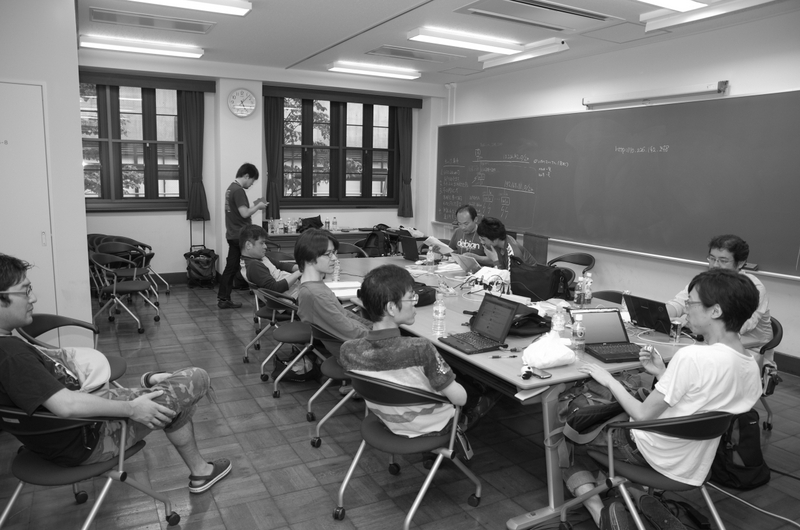
\includegraphics[width=0.8\hsize]{image201206/gum2012-hacklab_mono.jpg}

今回は、参加者向けのネットワークとして、無線 AP を用意して京都大学の Proxy 経由で外部に出ていくようにしていました。無線の調子は悪くなかったようですが、Proxy の設定でつまづく人はそれなりにいたようです。
また、WiMAX ルータを使って Ustream 中継をする予定にしていましたが、やはりというかセッション中は自前の Wifi ルータを使う参加者が多かったようで、接続が全く安定しませんでした。

\subsection{スケジュールとイベント}

開催期間は 1 日間のみで、Debconf のような催事はおりこまれていません。Debian 勉強会としては初の試みになりますが、2 トラックでのセッション運営を行い、合計 13 (加えて LT 5件) のセッションが行われました。

セッションの一環として、おなじみのキーサインパーティも開催され、28 名の参加者がありました。また、パーティには参加せず、個人的にキーサインを行う人もいたようです。

\subsection{セッション}

トラックを 2 つ設けたとはいっても、特にカテゴリの設定などはしませんでした。セッション内容も Debian 固有の開発話から Linux 全般に通じるネタ、組み込みやデバイス関連の Tips から便利なアプリケーションの紹介まで、千差万別でした。

セッションの内容は、下記の通りです。\footnote{http://gum.debian.or.jp/ のタイムテーブルに、当日の発表資料と titanpad によるディスカッションの記録が保存されています}

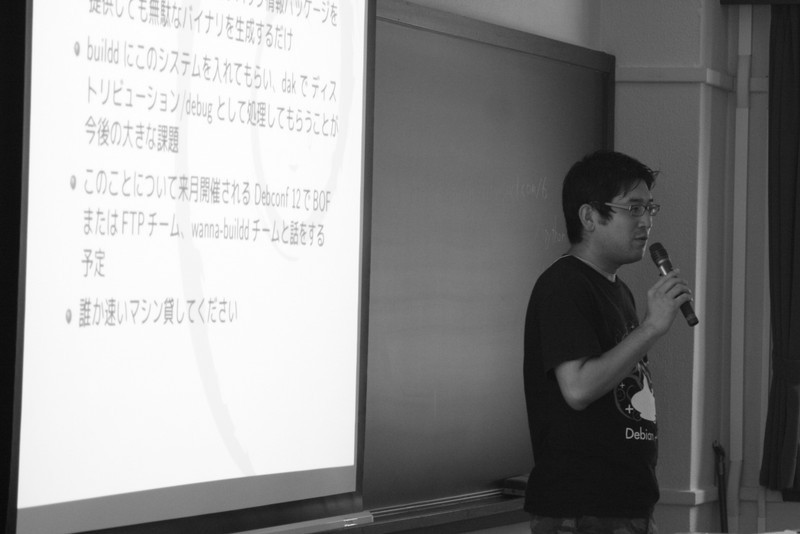
\includegraphics[width=8cm]{image201206/gum2012-session2_mono.jpg}
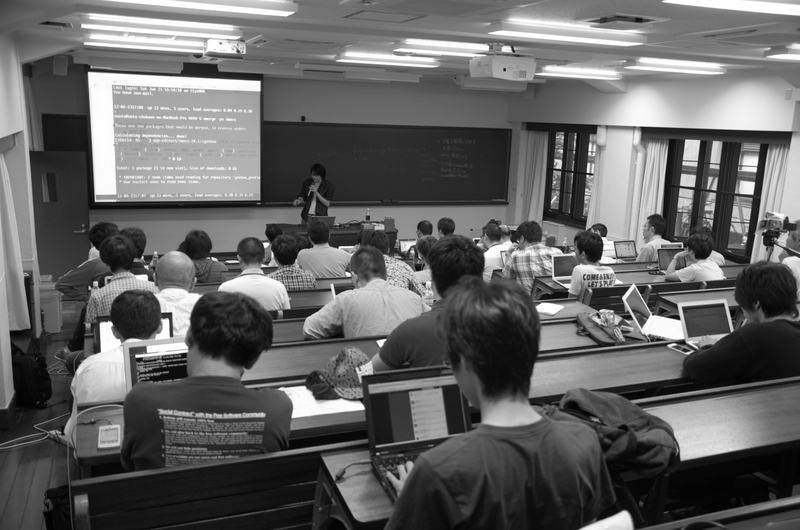
\includegraphics[width=8cm]{image201206/gum2012-session1_mono.jpg}

\subsubsection{TeXLive 2011(2012/dev) in Debian / 発表者 佐々木洋平}

pTeX がドロップされるなど、大きな変更が予定されている Wheezy 向けの \TeX 環境の現状紹介と、日本語処理面での導入、設定方法の説明がされました。

\subsubsection{Linux-PAM の設定について / 発表者 西山和広}

pam-auth-update など、独自のユーティリティに触れたりしつつも、PAM の構成や設定について、基本的なところから解説されていました。

\subsubsection{数学ソフトウェア使ってますか? / 発表者 濱田龍義}

最近 MathLibre と改名した、数学ソフトウェアに特化したライブディストリビューションと、収録されている数学ソフトウェアを紹介するセッションでした。

\subsubsection{ipython notebook とその周辺 / 発表者 本庄 弘典}

最近 Debian にインストールされた ipython notebookとその周辺ツールである ipython qtconsoleおよびipython nodebookの導入方法、使い方について説明
されました。

\subsubsection{Debian と LibreOffice / 発表者 あわしろ いくや}

OpenOffice から LibreOffice への変遷を軸に、Debian でのパッケージング状況や翻訳活動の紹介などが説明されていました。

\subsubsection{debug.debian.net / 発表者 岩松 信洋}

現在、Debian のバイナリパッケージは、コンパイル時にデバッグ情報が削除されています。デバッグなどの際に必要になるこのデータを提供しようというプロジェクトについての検討報告でした。休眠していた同様のプロジェクトを復活させる方向で動いているそうです。

\subsubsection{Rabbit: 時間内に終われるプレゼンツール / 発表者 須藤 功平}

どのようにプレゼンを行うのか、という観点も含めて Rabbit というプレゼンツールの背景にある設計思想を作者さん自らが解説する、というセッションでした。

\subsubsection{U-Bootについてあれこれ / 発表者 野島 貴英}

組み込み分野でよく利用されているブートローダである U-Boot の紹介と、Barnes \& Noble社Nook Color 向けに移植した例を紹介しました。

\subsubsection{Debian Multiarch Support / なかお けいすけ}

次期Debianのリリースゴールの一つに挙げられている Multiarch Support について仕組みと
現状について説明されました。

\subsubsection{家庭内LANを高速に! InfiniBand on Debian}

eBay で安価に機材を入手する方法から、Debian 上での利用方法、また高速な通信についての悦びまで、幅広く説明されていました。

\subsubsection{Gentoo/Prefix on Debian}

Gentoo Linux には、どんな OS にも Gentoo の皮をかぶせてしまう Prefix という仕掛け (平たく言うと chrooted gentoo) があります。
それを一歩進めて、Debian パッケージとの連携を深める試みについてのセッションでした。

\subsubsection{Debian でもマルチタッチ!}

Ubuntu が独自実装している関連パッケージを Debian にバックポートする方法の説明や、タッチパッドに指を何本も認識させるデモが行われていました。


\subsection{Lightning talk}
閉会直前に用意していた LT の枠も、事前の発表募集に反応が薄かったわりには当日の発表希望が複数あったため、なんとか無事に終えることができました。
LT のほとんどが Debian Developer によるものでしたが、これはさすがというべきか何というべきか....。

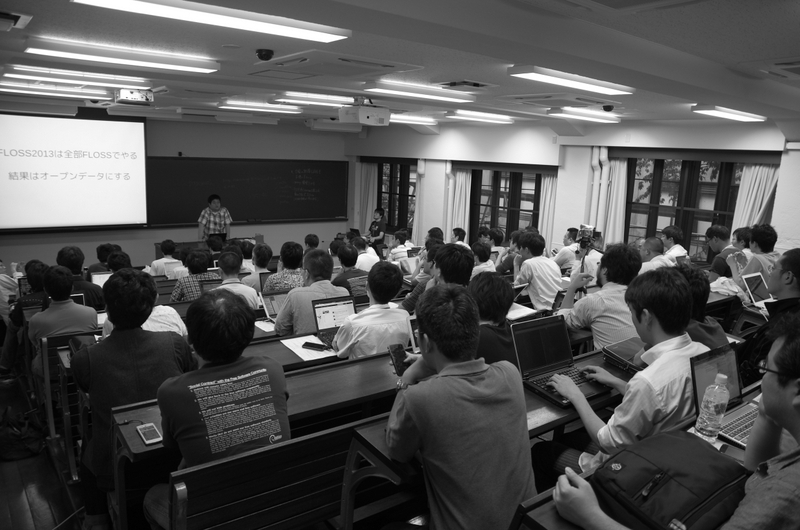
\includegraphics[width=8cm]{image201206/gum2012-lt_mono.jpg}
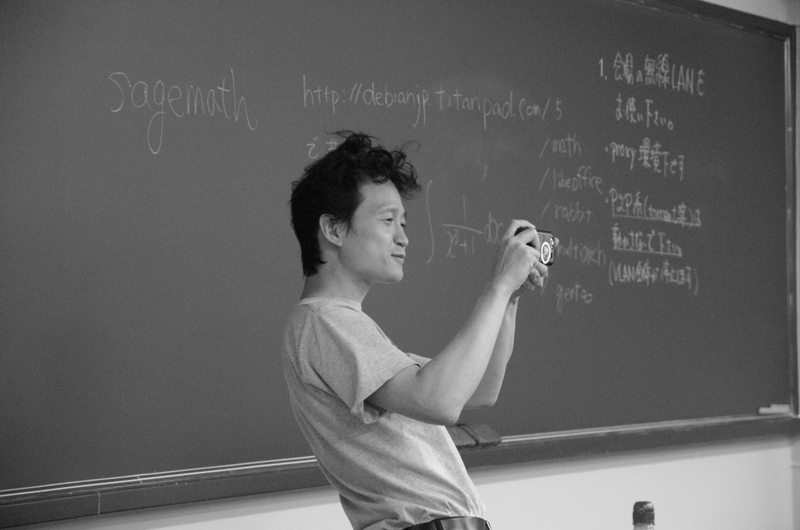
\includegraphics[width=8cm]{image201206/gum2012-closing_mono.jpg}

\subsection{懇親会}

閉会後、会場近くの居酒屋で懇親会を行いました。総勢 60 名弱の参加者があり、普段の勉強会とは一味違うもりあがりを見せていました。

\subsection{次回の大統一 Debian 勉強会}

今のところ、次回の予定はたっていません。今回を盛況のうちに終えることができたので、何らかの企画はなされるはずです。乞うご期待。

%-------------------------------------------------------------------------------
\dancersection{Debian Conference 2012参加報告}{岩松 信洋}
%-------------------------------------------------------------------------------

\label{sec:debconfreportsummary}
\index{Debconf2012}
\index{Debconf}

\subsection{Debconfとは}

2012年度の Debconf は 7月8日から7月14日まで、ニカラグアのマナグアで行われました。
日本からは、安井 卓、大岩 達也、矢吹 幸治、山根 秀樹、岩松 信洋が参加しました。

\subsubsection{Debconfの歴史・経緯}

Debian Conference \url{http://debconf12.debconf.org/} は Debian 
の開発者たちが一同に介するイベントです。通常顔をあわせることのないメンバー
たちが一同に介し友好を深め、技術的な議論を戦わせます。過去の開催履歴を見
てみると\tbref{tab:debconflist}のようになります。

\begin{table}[H]
\caption{歴代のDebconf参加者推移}
\label{tab:debconflist}
 \begin{center}
 {\footnotesize
 \begin{tabular}{|c|c|c|r|}
 \hline
 年 & 名前 & 場所 & 参加人数 \\
 \hline
 2000 & debconf 0 &フランス ボルドー & \\
 2001 & debconf 1 &フランス ボルドー & \\
 2002 & debconf 2 &カナダ トロント & 90名 \\
 2003 & debconf 3 &ノルウェー オスロ & 140名 \\
 2004 & debconf 4 &ブラジル ポルトアレグレ &  150名 \\
 2005 & debconf 5 &フィンランド ヘルシンキ & 200名 \\
 2006 & debconf 6 &メキシコ オアスタペック & 300名 \\
 2007 & debconf 7 &英国スコットランド エジンバラ & 約400名 \\
 2008 & debconf 8 &アルゼンチン マルデルプラタ & 約200名 \\               
 2009 & debconf 9 &スペイン エクストラマドゥーラ & 約250名 \\
 2010 & debconf 10 &アメリカ ニューヨーク & 約400名 \\
 2011 & debconf 11 &ボスニア バニャルカ & 約450名 \\
 2012 & debconf 12 &ニカラグア マナグア & 約180名 \\
 \hline
 \end{tabular}
 }
 \end{center}
\end{table}

\subsection{ニカラグア/マナグア}

\subsubsection{行き方}
日本からの行く場合、米国のマイアミかヒューストンからの入国が一番楽
なようです。他の国からは、コスタリカのサンホセやパナマ、アトランタ
から入国できます。
開催施設へはマナグアの空港から約20分ほどタクシーに乗る必要があります。
バスなどもありますが、地元の人の利用者が多いのと治安が悪いためあまり
使わないほうがよいとのこと。
今回ホテルのタクシーに送迎してもらいましたが、地元のタクシーの場合は
10ドルほどの料金がかかります。

\begin{figure}[ht]
\begin{center}
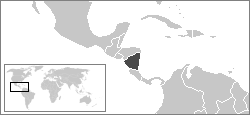
\includegraphics[width=0.8\hsize]{image201208/debconf12_LocationNicaragua_mono.png}
\caption{ニカラグア/マナグアの位置}
\end{center}
\end{figure}
%http://wikitravel.org/ja/%E3%83%95%E3%82%A1%E3%82%A4%E3%83%AB:LocationNicaragua.png

\subsubsection{会場}

\begin{wrapfigure}{r}{11cm}
  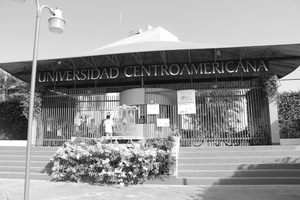
\includegraphics[width=5cm]{image201208/debconf12_mainentry_mono.jpg}
\end{wrapfigure}

2012年度のDebconfの会場はマナグアにある大学「UCA(Universidad Centroamericana」の施設の一部を借りて
行われました。宿泊は会場から5分ほど歩いた場所にあるホテル「Hotel Seminole」で行いました。
以下に会場を紹介します。
\\

\begin{itemize}
  \item Aula Magna Auditorium: メイン用。400人ほど入ることができます。\\
	\begin{minipage}{0.4\hsize}
	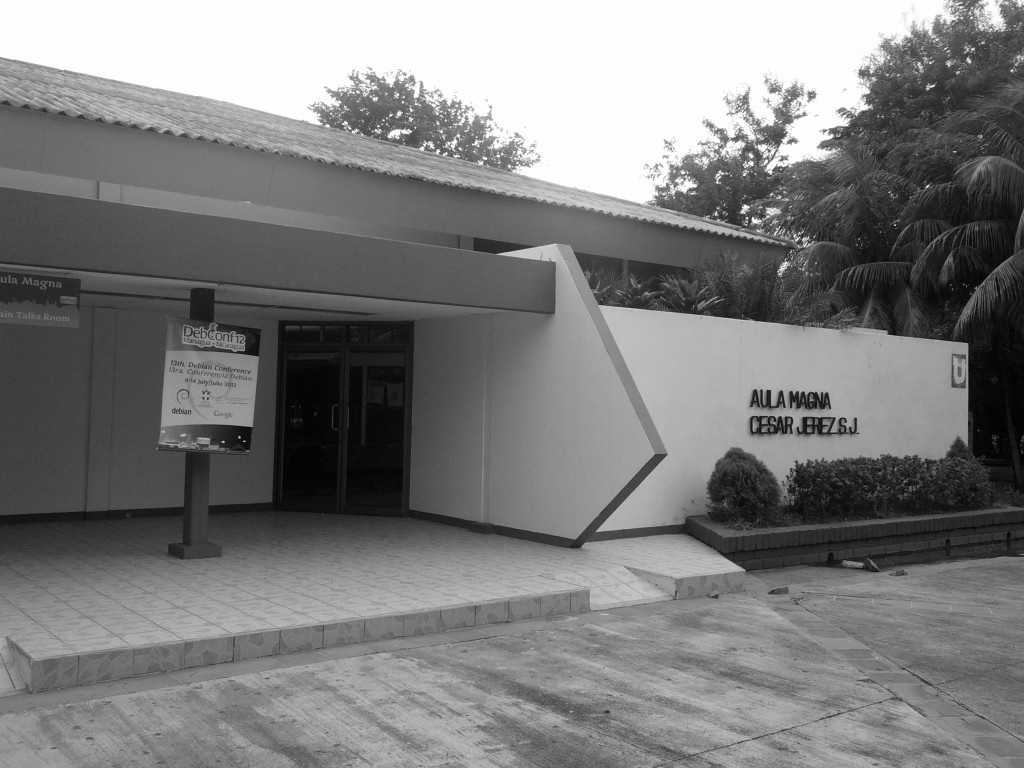
\includegraphics[width=0.8\hsize]{image201208/debconf12_maintalk01_mono.jpg}
        \end{minipage}
        \begin{minipage}{0.4\hsize}
        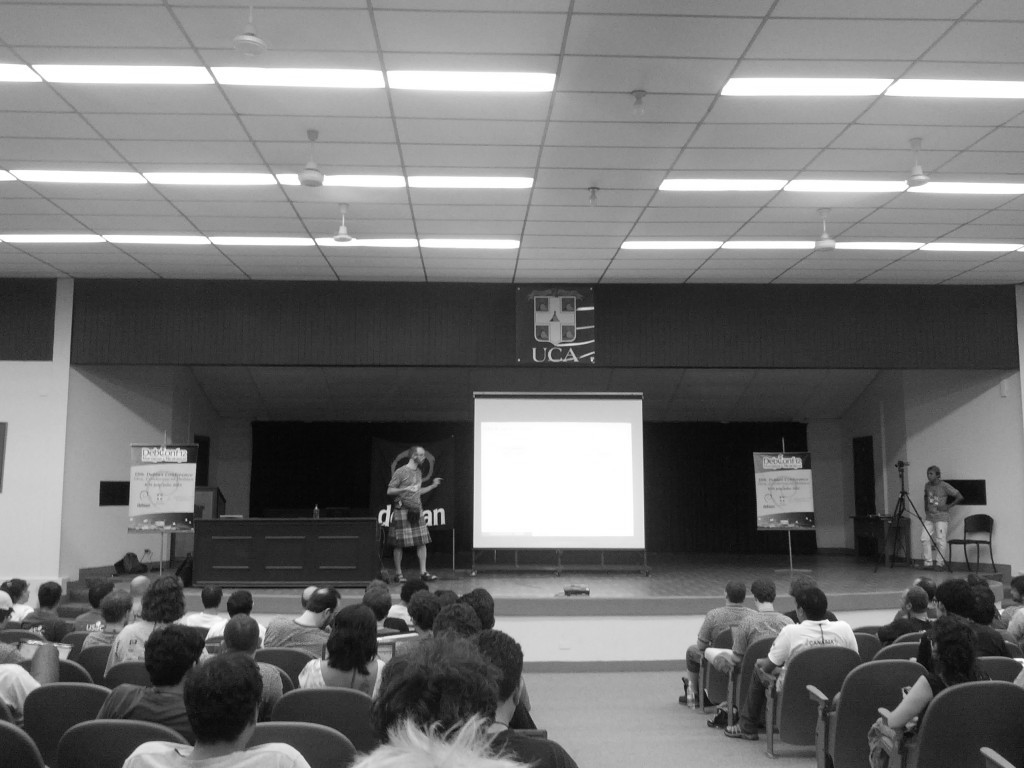
\includegraphics[width=0.8\hsize]{image201208/debconf12_maintalk02_mono.jpg}
	\end{minipage}

  \item Roberto Teran Auditorium: サブ会場。50人ほど入ることができます。\\
        \begin{minipage}{0.4\hsize}
        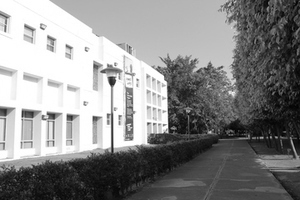
\includegraphics[width=0.8\hsize]{image201208/debconf12_2ndtalkroom01_mono.jpg}
	\end{minipage}
        \begin{minipage}{0.4\hsize}
        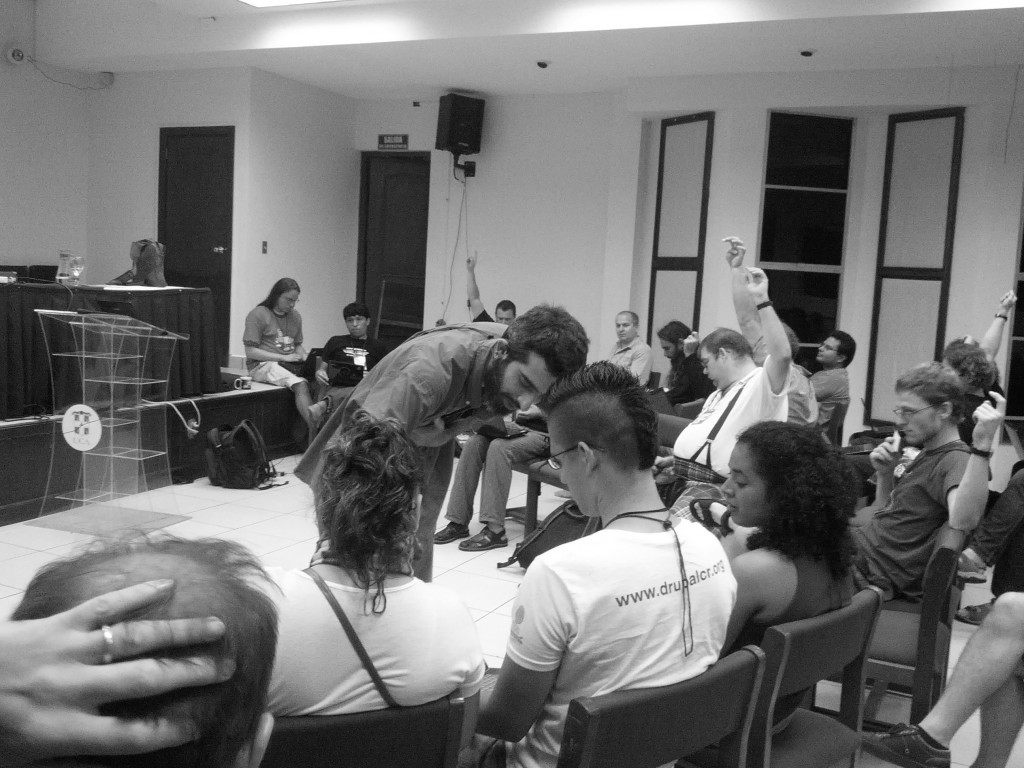
\includegraphics[width=0.8\hsize]{image201208/debconf12_2ndtalkroom02_mono.jpg}
	\end{minipage}

  \item Hacklab: Hacklab はハック専用の部屋です。\\
	\begin{minipage}{0.4\hsize}
	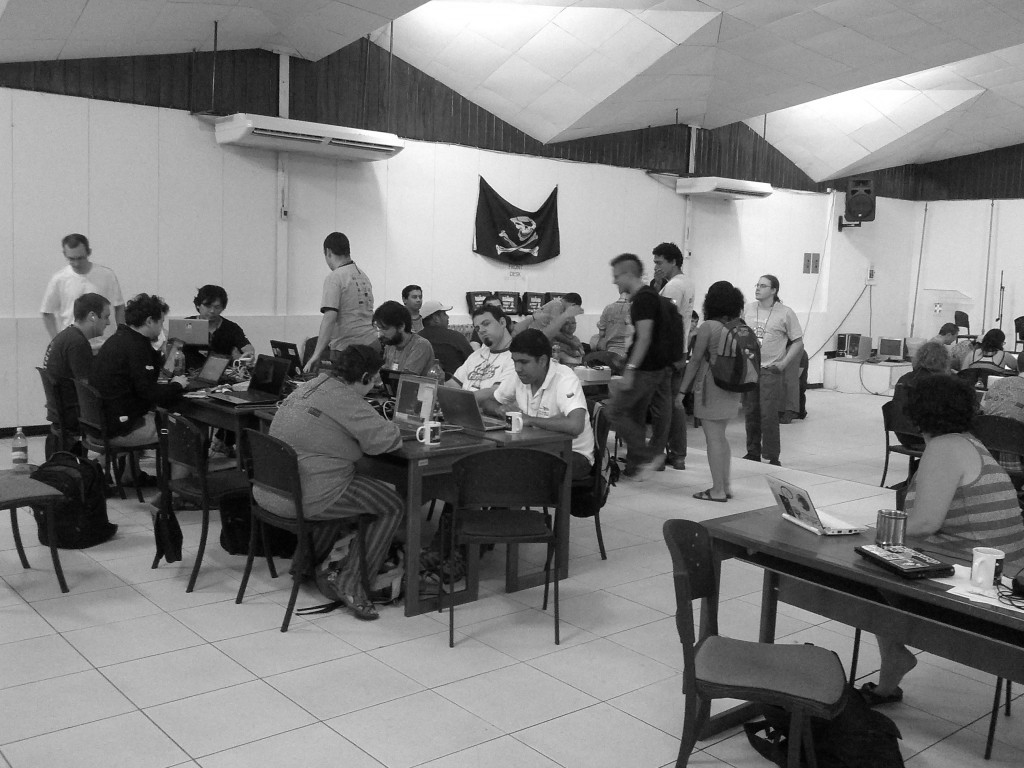
\includegraphics[width=0.8\hsize]{image201208/debconf12_hacklab01_mono.jpg}
	\end{minipage}
        \begin{minipage}{0.4\hsize}
        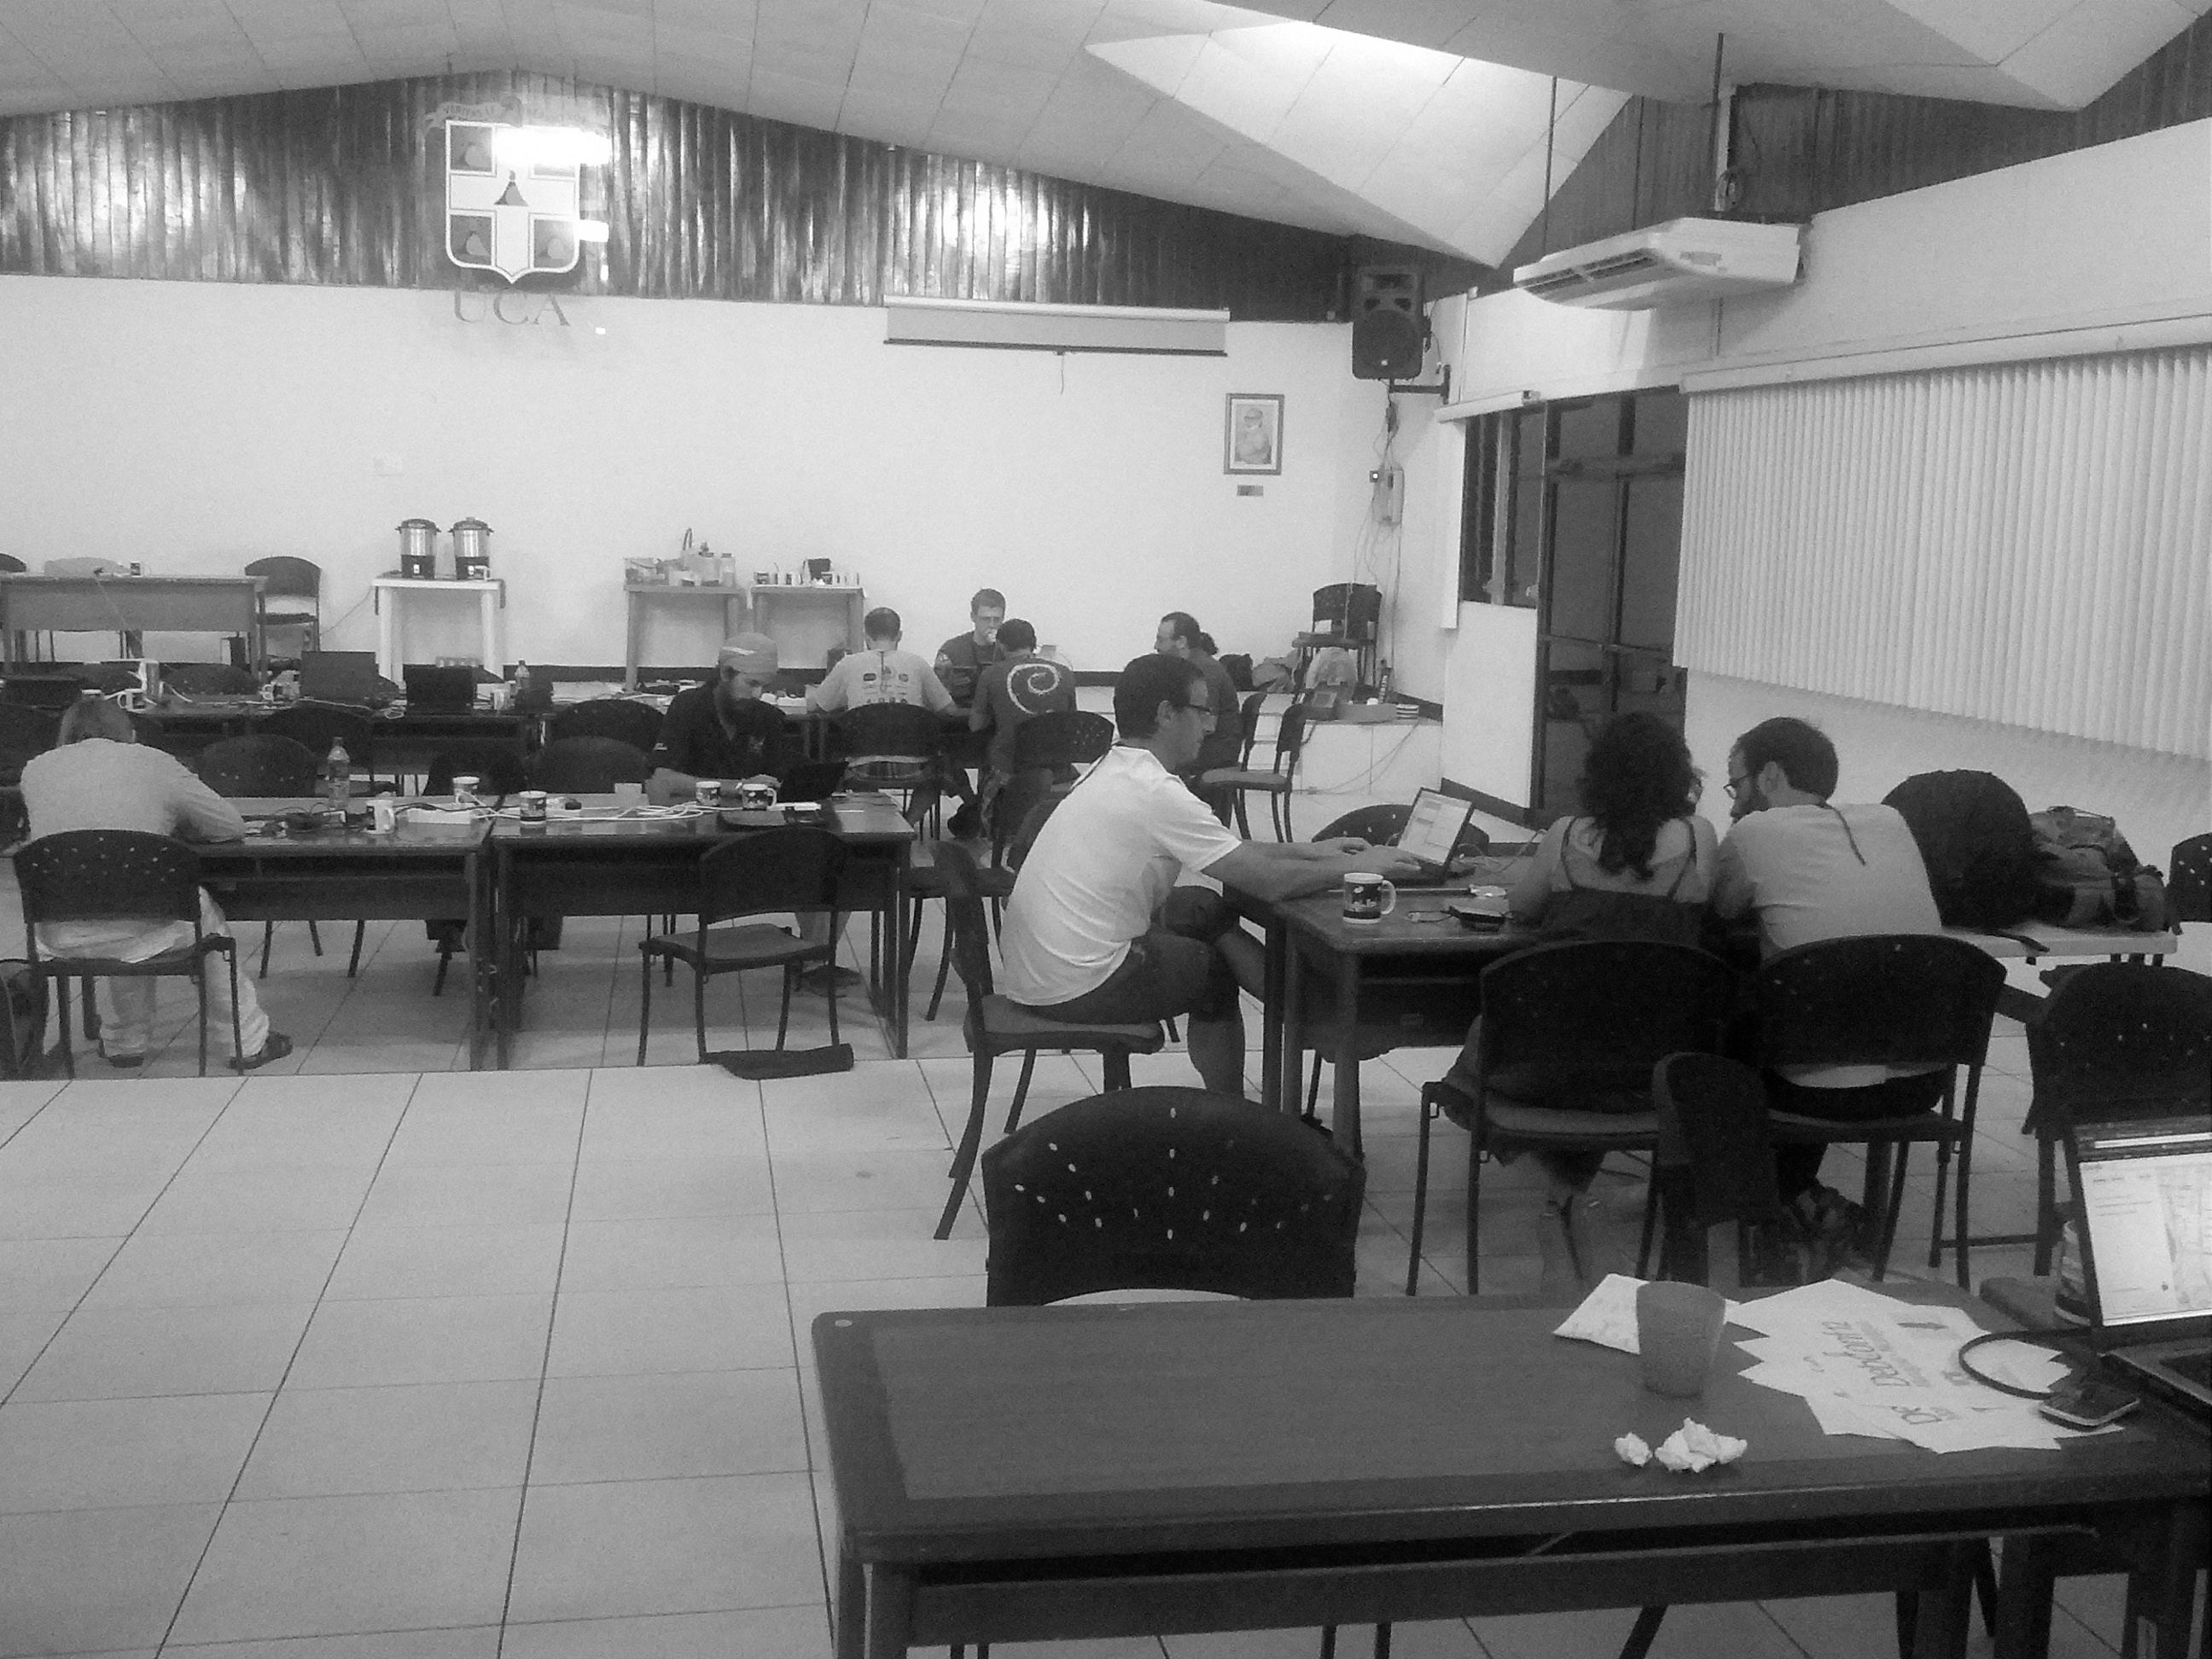
\includegraphics[width=0.8\hsize]{image201208/debconf12_hacklab02_mono.jpg}
	\end{minipage}

 \item 食堂: 食堂は外にテントを張って、そこで食事しました。\\
	\begin{minipage}{0.4\hsize}
	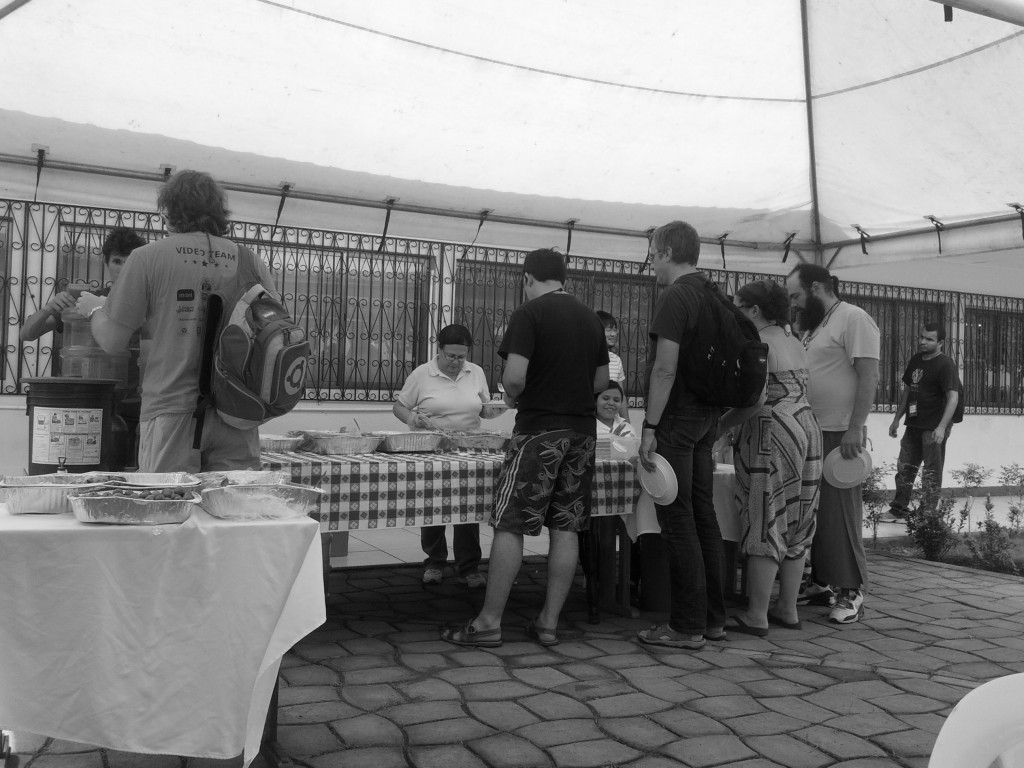
\includegraphics[width=0.8\hsize]{image201208/debconf12_diningroom01_mono.jpg}
	\end{minipage}
	\begin{minipage}{0.4\hsize}
	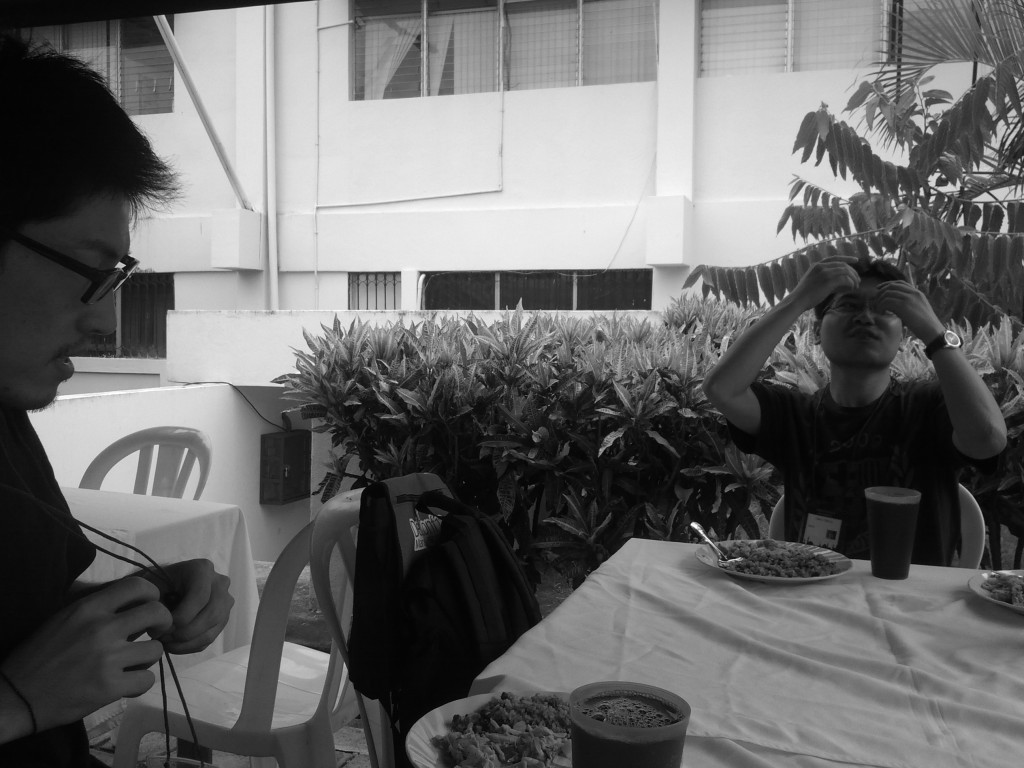
\includegraphics[width=0.8\hsize]{image201208/debconf12_diningroom02_mono.jpg}
	\end{minipage}


 \item 宿泊したホテル:\\
	\begin{minipage}{0.4\hsize}
	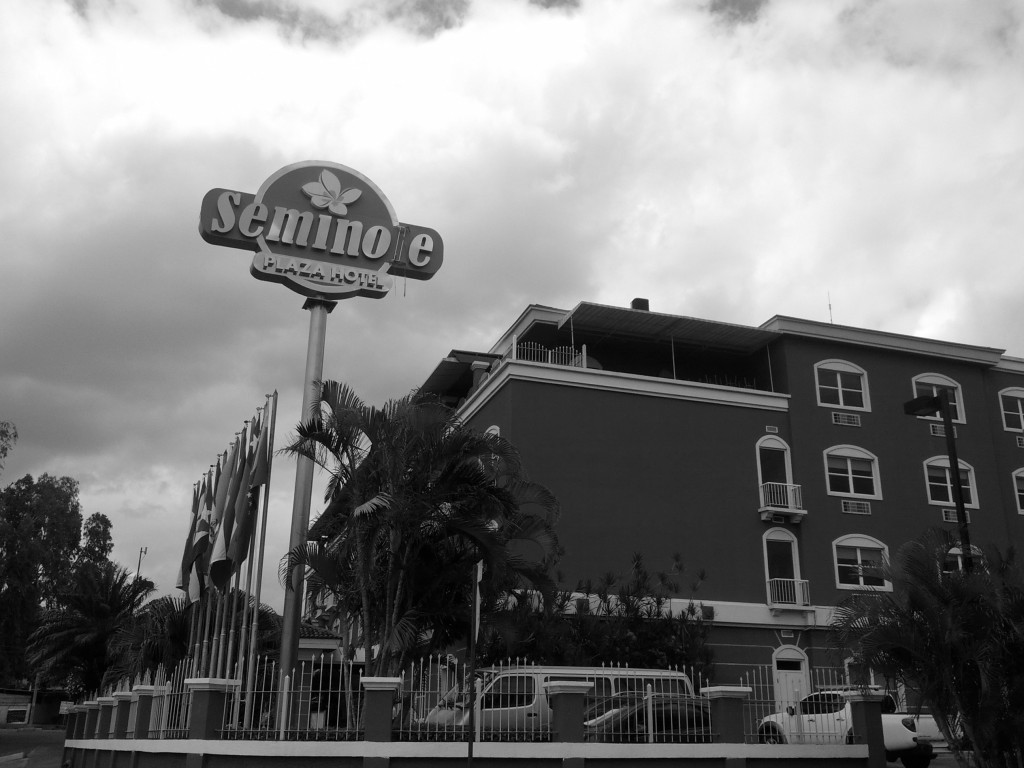
\includegraphics[width=0.8\hsize]{image201208/debconf12_hotel_mono.jpg}
	\end{minipage}
        \begin{minipage}{0.4\hsize}
        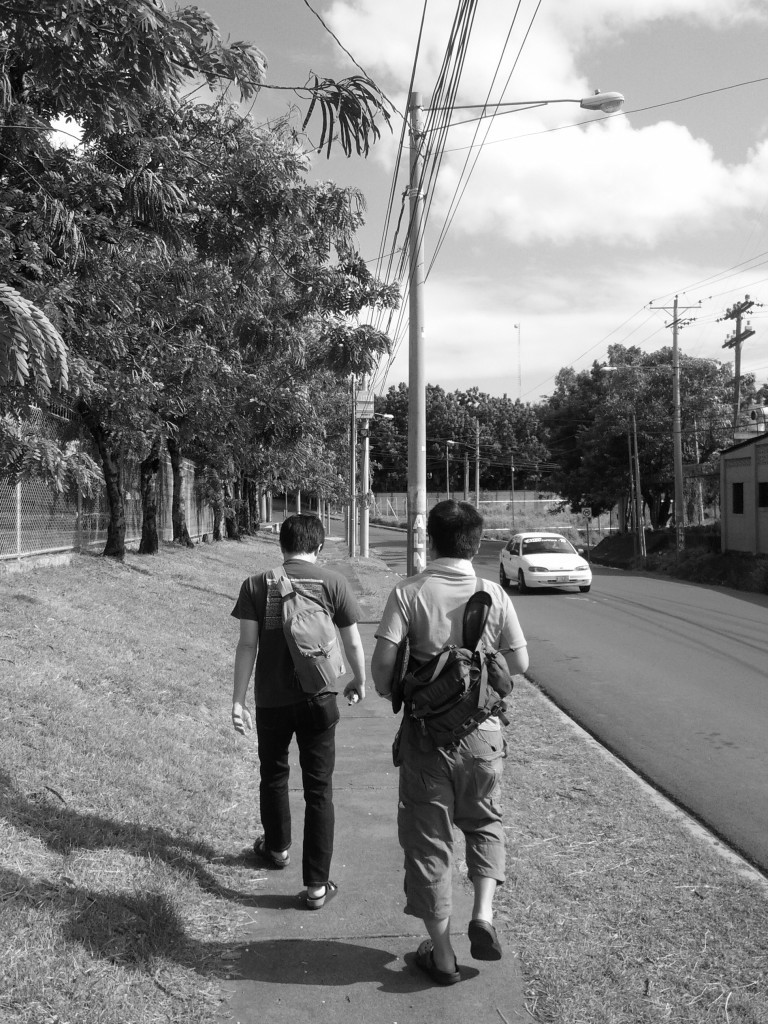
\includegraphics[width=0.8\hsize]{image201208/debconf12_hotel2_mono.jpg}
        \end{minipage}

\end{itemize} 

\subsection{スケジュール}

7日のDebian Day で Debian Conference は開幕し、14日まで毎日いろいろな予
定が組まれていました。
11日だけはカンファレンス参加者で Day-trip を実施しました。

\subsection{主となった討論}

今回のDebconfは議論テーマを2日目は組み込み、4日目は
バーチャライゼーションなど、日によって分けられる方式が取られました。
また、地元からの参加者もわかるようにスペイン語での発表も多くありました。
個人的に今回のDebconfはあまり興味がある話題がなく、面白そうな話題があま
りなかったように感じました。その中でも私が参加した会議の内容からいくつか
取り上げて紹介します。

\subsubsection{Bits from the Release Team}

リリースチームによる次期リリースに関する発表が行われました。
今回のリリースから kibi(Cyril Brulebois)がリリースアシスタントに
加わることが発表されました。
また、Debconf開催前にフリーズが行われ、次のリリース内容についても発表がされ
ました。主要なソフトウェアを挙げると、KDEは4.8、GNOMEは3.4、Linux kernelは
3.2となります。RCバグ(当時で603個)が多く残っているため、バグつぶしに協力
して欲しいと報告が行われました。

\subsubsection{EFI BOF}
EFI(UEFI)についてのBOFが行われました。EFIのSecure boot に対応する
ためにはどのようにしたらいいのか、他のディストリビューションの対応
とDebian での対応方法について情報交換が行われました。
RedHat/Fedoraはブートローダと全てのカーネルスタックに署名する方法で対応
しているようです。またCanonical/Ubuntuはefilinuxのみに署名し対応する方法
を取っているとのこと。GPLv3の問題もありGrub2での対応は難しそうです。
今回のBOFでは良い案は出て来ませんでした。

\subsubsection{Multiarch crossbuilding}
Wookeyによる multiarch がサポートされた環境でのクロスビルドパッケージの
状況と問題点について発表が行われました。
現在 rebuildd と sbuild を使った クロスビルドファームを立ち上げ、クロス
ビルドテストを行なっていますが、まだいくつかの課題があるようです。
例えば multiarch のforeign
に対するクロスコンパイルに必要なパッケージの指定方法などに課題があります。
これを解決するためにパッケージのメタ情報として、cross-build-dep を指定し
これをaptで処理できるようにする機構を追加する(\#666772)といった方法があります。まだいくつか問題が残っているので協力して欲しいとのことでした。

\subsubsection{Build Debian with another compiler}
Sylvestre Ledru による LLVM を使ったDebianパッケージの全ビルドについて
の発表。現在、DebianのデフォルトのCコンパイラはGCCですが、LLVM/Clang 
を使ってみた結果と今後の予定について発表されました。
LLVMを使う理由として、ビルド速度が少しだけ速いということや、GCCより
より賢いコードパース機能が挙げられます。またGCCではない高性能な
コンパイラを選択できるということも良い点です。
Sylvestreは実験Debconf前に行われた LLVM 3.0 と3.1 の結果を元に
LLVMの利点を説明しました。
2012年の2月の時点でLLVM 3.0では、15658パッケージ中1381パッケージ 
(全体の8.8 \%)がビルドエラーになっているとのこと。
ほとんどのパッケージがビルドできているようです。
また 2012年の6月に行ったLLVM 3.1 では
17710 パッケージ中 2137パッケージ (全体の12.1 \%) がビルドに失敗している
ようです。この違いが出た理由は一部のオプションがサポートされていなかったり、
LLVM 3.0 では出なかったプログラムのバグ(プログラムミス)が検知できるよう
になったためです。
結果を\url{http://clang.debian.net/}から参照できます。
発表された時点では、まだGCCと切り替えできる機構が整備されていないため、
まだコンパイラ単体じゃないと利用できませんでした。今後は sbuild や dpkg
などのビルドツールにLLVM サポートを入れるように活動するとのこと。
商用コンパイラであるIntel コンパイラを使うためのツールやビルドも行なっている
ようなので、気になる方はSylvestreに連絡をとってみてください。
 
\subsubsection{ARM port(s) update}
ARMチームによる ARM ポーティングの状況について報告が行われました。
現在armelとarmhfの2つのアーキテクチャがあり前者は古いARM SoC(v4t)
を、後者は比較的新しいARM SoC(v7) をサポートしています。
armel はまだユーザもいるので今後もサポートしていく予定です。armhf は
次のリリースに含まれる予定ですが、動作させているマシンのメモリが1GB
しかないため、いくつかのソフトウェアがビルドできない等の問題が起きてい
るようです。この問題を解決するために ARM Server 向けのマシンをどこかから
(HPと交渉しているようだけど)借りて、Builddを置き換える予定みたいです。
この話の背景として、今後はモバイル端末だけでなく Server でもARMが使われる
ようになるため、それらをDebianでサポートするためのことも考えているとのこと。
その他、Raspbianや他のディストリビューションのサポート状況などについても
情報交換されました。

\subsubsection{AArch64 planning}
ARM 64bit サポートアーキテクチャである AArch64 サポートの
報告が行われました。AArch64 は ARMv7互換の64bit CPU ARMv8をサポート
するためのLinuxアーキテクチャ名です(LKMLでこの名前はどうなの?
と議論されていましたが)。まだCPUはまだ開発中で来年の頭に市場に投入される
と言われています。これを次のリリースである Jessie のサポートアーキテクチャ
にするためにARMチームは活動していると報告しました。
現在Linuxカーネル、ツールチェイン、dpkg、autoconf のサポートは完了して
おり、Qemuベースで動作しているとのこと。実際にそのデモも行われました。

\subsubsection{FreedomBox Update}
Bdale Garbee による FreedomBox の報告が行われました。
FreedomBox は Dreamplug などのARM Soc を使ったプラグ型サーバの
Linux ディストリビューションです。プライベートデータを
容易に扱うことのできるサーバを構築できることを目的としています。
今回、FreedomBoxを開発するための団体である FreedomBox Foundation の
紹介とFreedomBoxの成果をDebianにマージ完了の報告が行われました。
現在Dreamplugしかサポートしていませんが、今後他のマシンの対応もすると
のことです。

\subsection{Debconf14}
Debconf14 はマルティニーク(カリブ海の島。フランス領)、 
カナダのモントリオール、ベネズエラのプエルトラクルスが立候補しました。
マルティニークは飛行機でいくのが難しそうな国なのと十分なネットワーク
環境がないのでいまのところ難しそうです。モントリオールは設備がまだ不十分な
感じです。ベネズエラは既に国内のスポンサーも獲得しており、ホテルもいくつか
抑えてるとのこと。ネットワーク以外は網羅していると思いました。

\subsection{Daytrip}

\begin{minipage}{0.4\hsize}
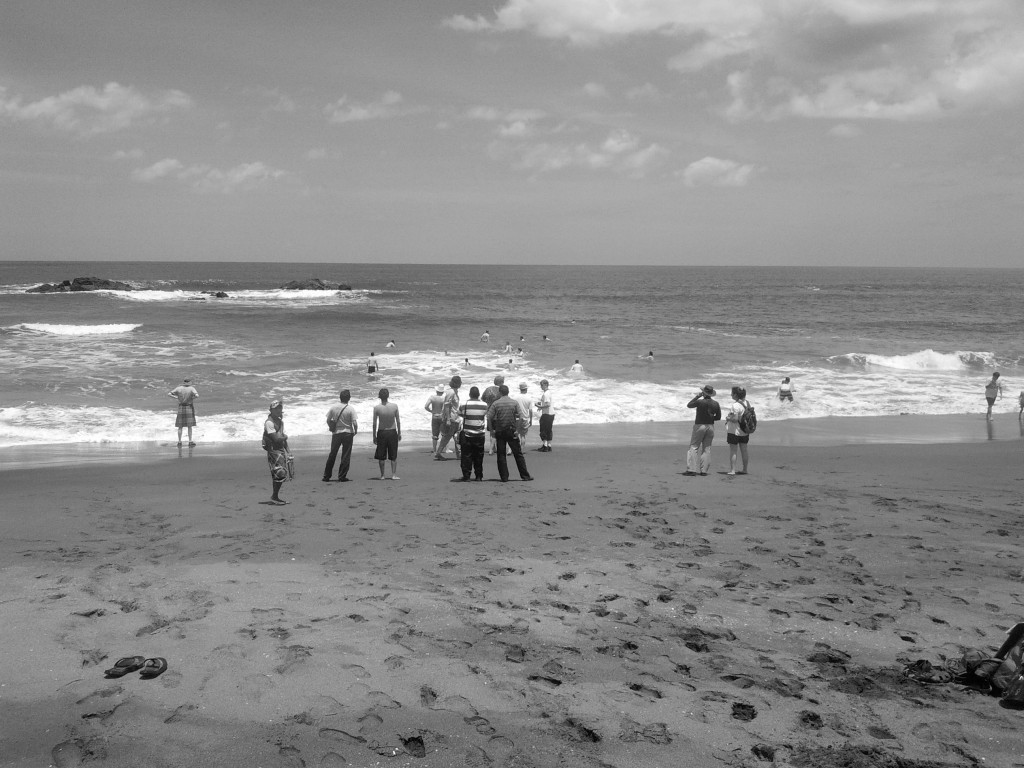
\includegraphics[width=0.8\hsize]{image201208/debconf12_daytrip01_mono.jpg}
\end{minipage}
\begin{minipage}{0.4\hsize}
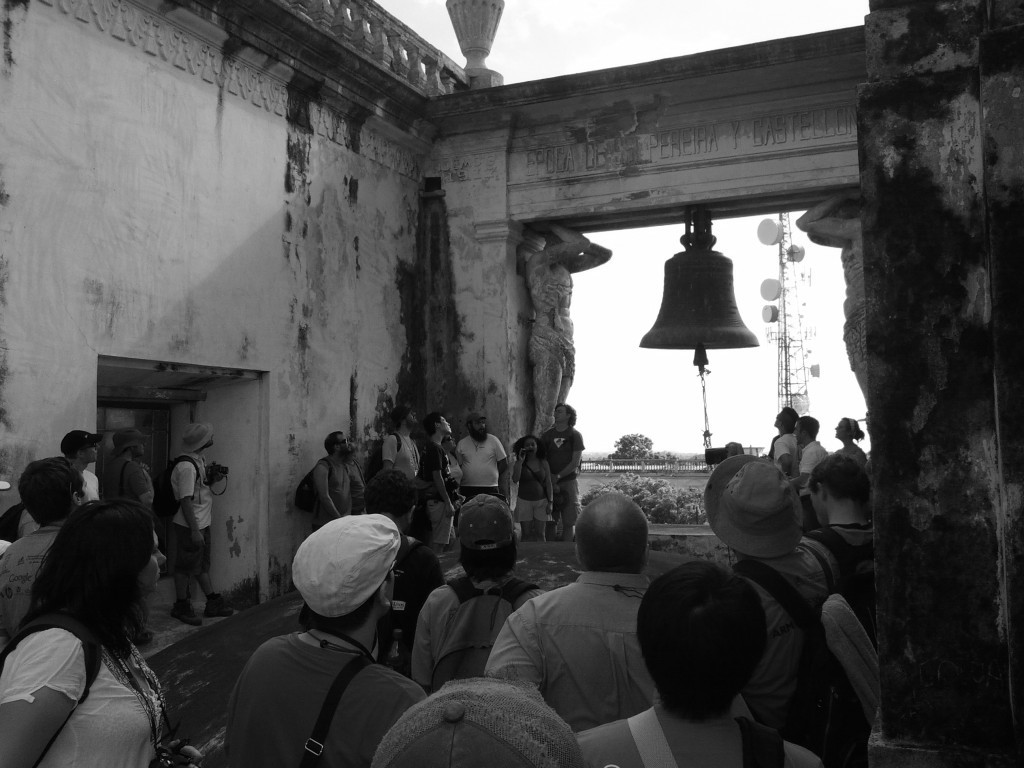
\includegraphics[width=0.8\hsize]{image201208/debconf12_daytrip03_mono.jpg}
\end{minipage}

Debconf では一日、参加者で旅行をするというイベントがあります。今回の
Debconfでは レオン旧市街観光ツアー、火山観光ツアー、ジュアンベアノ島
観光ツアーのチームに別れ、Daytrip をしました。
矢吹以外の日本からの参加者は全員火山観光ツアーに登録しましたが、先日の
大雨の影響で火山ツアーは行く事ができず、海に行ったあとにレオン市街観光
を行いました。

\subsection{次回のDebconf}
次回のDebconf13はスイスのヴァーマルキュで開催される予定です。
日程は8月5日から18日です。キャンプ場を借りきってやるようですが、
周りに何もないように見えます。
ホテルという施設でもないのでシェラフ等を持っていく必要がありそうです。
普段とは異なったサバイバルになると思います。

%-------------------------------------------------------------------------------
\dancersection{Debian Trivia Quiz}{上川 純一、岩松 信洋}
%-------------------------------------------------------------------------------

ところで、みなさん Debian 関連の話題においついていますか?Debian関連の話
題はメーリングリストをよんでいると追跡できます。ただよんでいるだけではは
りあいがないので、理解度のテストをします。特に一人だけでは意味がわからな
いところもあるかも知れません。みんなで一緒に読んでみましょう。

今回の出題範囲は\url{debian-devel-announce@lists.debian.org} や \url{debian-devel@lists.debian.org}に投稿された
内容とDebian Project Newsからです。

\begin{multicols}{2}
%; whizzy-master ../debianmeetingresume201210.tex
% 以上の設定をしているため、このファイルで M-x whizzytex すると、whizzytexが利用できます。
%

\santaku
{9/29 に行われた Debian 6.0 のアップデートは何回目でしょうか。}
{5}
{6}
{7}
{B}
{6.0.6 です。}

\santaku
{DMUA フィールドがなくなり、Debian Maintainerのアップロードが変更されます。今後、アップロードの際にどのように作業する必要があるか?}
{FTP masterに電話}
{スポンサーに dak の処理を依頼する}
{専用アップローダにアップロード}
{B}
{}

\santaku
{IRC 経由でVCS リポジトリを監視するサービスで終了したものは?}
{ICPO}
{NPA}
{CIA}
{C}
{KGBに移行。ICPA:  International Criminal Police Organization, NAP:National Police Agency, CIA: Central Intelligence Agency}

\santaku
{Debian Policy メンテナに新しく入ったのは誰か?}
{Kei Hibino}
{Colin Watson}
{Charles Plessy}
{C}
{Andrew McMillan, Colin Watson, Manoj Srivastava が抜けた}

\santaku
{Checksums-SHA1,SHA256 の取り扱いが変更になったが、どう変更されたか?}
{今まで無視されていました。ごめんね。}
{オプションだったので、必須としました。}
{これらは廃止し、SHA-512のみにします。}
{B}
{Bug\#690293}

%; whizzy-master ../debianmeetingresume201211.tex
% $B0J>e$N@_Dj$r$7$F$$$k$?$a!"$3$N%U%!%$%k$G(B M-x whizzytex $B$9$k$H!"(Bwhizzytex$B$,MxMQ$G$-$^$9!#(B
%

\santaku
{FTP master $B$K$"$?$i$7$/;22C$7$?$N$O(B}
{iwamatsu}
{ansgar}
{bdale}
{B}
{Ansgar $B$,?7$7$/;22C$7$^$7$?!#(Bmhy, joerg, ansgar $B$N;0?MBN@)$K(B}

\santaku
{pdiff$B$G2?$,2~A1$5$l$?$+(B}
{$B:GBg(B2$B$D$N(BDiff$B$r%@%&%s%m!<%I$9$l$PNI$$$h$&$KJQ99$K$J$C$?(B}
{$B0lF|(B10$B8D$E$D(BDiff$B$r@8@.$9$k$h$&$K$J$C$?(B}
{Diff$B$C$F$J$K$=$l$*$$$7$$$N!)(B}
{A}
{apt-get update $B$NCY$5$,%^%7$K$J$j$^$9$M!#(B}

\santaku
{CTTE 573745 $B$G2?$,7hDj$5$l$?$+(B}
{Mattias Klose $B%/%S(B}
{python $B=*N;$N$*CN$i$;(B}
{$B$_$s$JCgNI$/$7$h$&$M(B}
{C}
{python $B$N%a%s%F%J$N%3%_%e%K%1!<%7%g%sITB-$K$D$$$F$N5DO@$O7k6I$_$s$JCgNI(B
$B$/$7$^$7$g$&$H$$$&7kO@$K$J$j$^$7$?$M!#(B}

\santaku
{$B?7$7$/(BFront Desk$B$N%a%s%P!<$K$J$C$?$N$O(B}
{Kouhei Maeda}
{Iwamatsu}
{Jonathan Wiltshire}
{C}
{4$B?M$K$J$j$^$7$?!'(B
 Bernd Zeimetz      (bzed)
 Enrico Zini        (enrico)
 Jan Hauke Rahm     (jhr)
 Jonathan Wiltshire (jmw)
}

\santaku
{debian installer 7.0 beta3 $B$N?75!G=$G$O$J$$$N$O$I$l$+(B}
{ipv6}
{UEFI}
{grub2}
{C}
{}

\santaku
{}
{}
{}
{}
{}
{}
\santaku
{}
{}
{}
{}
{}
{}
\santaku
{}
{}
{}
{}
{}
{}
\santaku
{}
{}
{}
{}
{}
{}

\end{multicols}

% 問題と回答が同じみひらきにならないようにする
\cleartoevenpage
%-------------------------------------------------------------------------------
\dancersection{Debian Trivia Quiz 問題回答}{上川 純一、岩松 信洋}
%-------------------------------------------------------------------------------

 Debian Trivia Quiz の問題回答です。
 あなたは何問わかりましたか? \\
 %回答はdebianmeetingresume2012-fuyu.jqzというファイルに生成されるので、
 %それを手動でコピペして使う。
 % ここからコピペ
 % FIXME 問題が全部はいったらコピペすること
 %(progn (next-line 1)(insert-file "debianmeetingresume2012-fuyu.jqz") )
1. B 6.0.6 です。\\
2. B \\
3. C KGBに移行。ICPA: International Criminal Police Organization, NAP:National Police Agency, CIA: Central Intelligence Agency\\
4. C Andrew McMillan, Colin Watson, Manoj Srivastava が抜けた\\
5. B Bug\#690293\\
6. B Ansgar が新しく参加しました。mhy, joerg, ansgar の三人体制に\\
7. A apt-get update の遅さがマシになりますね。\\
8. C python のメンテナのコミュニケーション不足についての議論は結局みんな仲良くしましょうという結論になりましたね。\\
9. C 4人になりました:Bernd Zeimetz (bzed) Enrico Zini (enrico) Jan Hauke Rahm (jhr) Jonathan Wiltshire (jmw) \\
10. C \\
11. A \\
12. B \\
13. A \\
14. A \\

\printindex

% add page to even number
\newpage
\thispagestyle{empty}\mbox{}

\newpage
%\thispagestyle{empty}\mbox{}
%\newpage

\thispagestyle{empty}
{
\large
\begin{itembox}{\bf 『あんどきゅめんてっど でびあん』について}
本書は、東京および関西周辺で毎月行なわれている『東京エリア Debian 勉強会』および
『関西 Debian 勉強会』で
使用された資料・小ネタ・必殺技などを一冊にまとめたものです。
収録範囲は2012/07〜2012/11まで
東京エリアは第90回から第94回まで(第92回はOSC 2012 Tokyo/Fallのため収録無し)およびDebian パッケージング道場、関西エリアは第61回から第65回まで(第66回はKOF 2012のため収録無し)。
% FIXME: 回数を修正すること。
内容は無保証、つっこみなどがあれば勉強会にて。
\end{itembox}
}

\vspace*{13cm}
{\color{dancerlightblue}\rule{\hsize}{1mm}}
\vspace{2mm}

\includegraphics[width=2cm]{image200502/openlogo-nd.eps}
\noindent \Large \bf あんどきゅめんてっど でびあん 2012年冬号\\
\noindent \normalfont 2012年12月31日 \hspace{5mm}  初版第1刷発行\\
\noindent \normalfont 東京エリア Debian 勉強会/関西Debian 勉強会 (編集・印刷・発行)\\
{\color{dancerdarkblue}\rule{\hsize}{1mm}}

\end{document}
